\documentclass{article}
\usepackage[english]{babel}
%\usepackage[utf8x]{inputenc}
%\usepackage{apacite}
\usepackage[toc,page]{appendix}
%\usepackage{biblatex} % place in the document preamble
%%---------- path ------------%%
%\def\input@path{{~/Dropbox/6_Graduate/}}
%%---------- my command --- ----------%%
\newcommand{\pard[1]}{\frac{\partial}{\partial{#1}}}
\newcommand{\mean[1]}{\frac{1}{n}\sum_{i=1}^{#1}}
\newcommand{\defeq}{\vcentcolon=}
\newcommand{\eqdef}{=\vcentcolon}
\newcommand\independent{\protect\mathpalette{\protect\independenT}{\perp}}
\newcommand{\wh}{\widehat}
\newcommand{\itl}{\intercal}
\newcommand{\p}{\prime}
\newcommand{\bs}{ \boldsymbol}
\newcommand{\mb}{\mathbb}
\newcommand{\ml}{\mathcal}
\newcommand{\br}{\bar}
\newcommand{\txt}{\text}
\newcommand{\lt}{\left}
\newcommand{\rt}{\right}
\newcommand{\lv}{\lvert}
\newcommand{\rv}{\rvert}
\newcommand{\nlim}{\underset{n \to \infty}{\lim}}
\newcommand{\smb}{\begin{bmatrix}}
	\newcommand{\sme}{\end{bmatrix}}
\newcommand\indep{\protect\mathpalette{\protect\independenT}{\perp}}
\def\independenT#1#2{\mathrel{\rlap{$#1#2$}\mkern2mu{#1#2}}}
\newcommand{\tsgn}{\txt{sgn}}


%%-------- my package -------%%
\usepackage{ragged2e}
\usepackage{float}
\usepackage{epstopdf}
\usepackage[final]{pdfpages}
%\usepackage{cite}
\usepackage{amsmath}
\usepackage{color}
\usepackage{graphicx}
\usepackage{verbatim}
\usepackage{commath}
\usepackage{caption}
%\usepackage{bbm}
%\usepackage{xfrac}
%\usepackage{dsfont}
\usepackage{amssymb}
\usepackage{verbatim}
\usepackage{mathtools}
\usepackage{resizegather}
\usepackage{xfrac}
\usepackage{amsthm}
\usepackage[ruled]{algorithm2e}
%\newtheorem{remark}{Remark}
%\newtheorem{lemma}{Lemma}
%\newtheorem{theorem}{Theorem}
%\newtheorem{corollary}{Corollary}
\newtheorem{theorem}{Theorem}[section]
\newtheorem{lemma}[theorem]{Lemma}
\newtheorem{proposition}[theorem]{Proposition}
\newtheorem{corollary}[theorem]{Corollary}
\renewcommand\qedsymbol{$\blacksquare$}

%%----------------------------------------------------------------------------%%
%%------------------------------ Import Packages -----------------------------%%
%%----------------------------------------------------------------------------%%


\usepackage{booktabs}  % professionally typeset tables
\usepackage{amsmath}
\usepackage{textcomp}  % better copyright sign, among other things
\usepackage{xcolor}
\usepackage{lipsum}    % filler text
\usepackage{subfig}    % composite figures


%%----------------------------------------------------------------------------%%
%%---------------------------- Formatting Options ----------------------------%%
%%----------------------------------------------------------------------------%%
%%

%% -------------------------------------------------------------------------- %%
%% Disposition format -- any titles, headings, section titles
%%  These formatting commands affect all headings, titles, headings,
%%  so sizing commands should not be used here.
%%  Formatting options to consider are
%%     +  \sffamily - sans serif fonts.  Dispositions are often typeset in
%%                    sans serif, so this is a good option. 
%%     +  \rmfamily - serif fonts
%%     +  \bfseries - bold face
%\dispositionformat{\sffamily\bfseries}   % bold and sans serif


%% ------------------------------
\title{Constrained Estimation of Single-stage Optimal Treatment Regimes}
\author{Shuping Ruan, Eric Laber\\ Department of Statistics, North Carolina State University}


\begin{document}
\maketitle

\section{Introduction}
Precision medicine tailors medical treatments to each patient's own characteristics. It categorize individuals into subpopulations based on, for example, their response to a specific treatment, or their susceptibility to a certain disease, etc. Hence, it targets therapeutic or preventive interventions to those who may benefit, and save those who may not benefit from unnecessary side effects and costs. Given a patient state, such as genetic information, demographics, results of diagnostic test, and so on, dynamic treatment regimes determine what treatment should be assigned next. These are data-driven decision rules that map patient characteristics to recommended treatments. \\

There is a rich body of research on estimating optimal treatment regimes using data from randomized clinical trials or observational studies. In most cases, a dynamic treatment regime is defined to be optimal if it maximizes the expected value of a certain cumulative clinical outcome when applied to a population of interest. Methods to estimate an optimal treatment regime include Q-learning~\cite{Nahum2012}, penalized Q-learning~\cite{Song2011}, interactive Q-learning~\cite{Linn2014}, A-learning~\cite{Schulte2014}, regret-regression~\cite{henderson2010}, g-estimation~\cite{gestimation}, and policy search methods~\cite{Zhao2012,Zhao2015,Zhang2012,Zhang2012b,Orellana2010a,Zhao2012}. However, these estimators seek to maximize the expectation of a single scalar outcome, and therefore, neglect the clinical need to balance several competing outcomes. For example, a clinician may have to balance treatment effectiveness, side-effect burden, and cost while developing a treatment strategy for a patient with a chronic disease; or maximize the expected time to an adverse event while controlling the variance of the time to the adverse event.\\

 Despite its practical importance, very little work has been done on handling multiple competing outcomes. Lizotte et al. considered linear combinations of two competing outcomes indexed by a trade-off parameter and compute the optimal treatment regime for all combination~\cite{Lizotte2010}. However, it may not be realistic to assume that a linear trade-off is sufficient to describe all possible patient preferences~\cite{LaberTwo2014}. Wang et al. used a compound score or ``expert score" by numerically combining information on treatment efficacy, toxicity, and the risk of disease progression~\cite{Wang2012}. Unfortunately, the elicitation of a good composite outcome can be difficult and the misspecification of a composite outcome may severely affect the quality of the estimated treatment regime~\cite{Laber2014}. There are also some methods to avoid formation of composite outcomes. Laber et al. proposed set-valued dynamic treatment regimes~\cite{LaberTwo2014}. This method inputs current patient information and outputs a set of recommended treatments. This set contains multiple treatments unless there exists a treatment that is best across all outcomes. This method may not be able to recommend a single treatment and needs expertise for tie breaking when a set of several treatments are recommended. Also, it needs to specify ``clinically significant differences" for competing outcomes. Linn at el. proposed constrained interactive Q-learning algorithm~\cite{Linn2014a}, which provides an algorithm to find the optimal regime under constraints in the two-stage setting.\\

We propose a new statistical framework to tackle the problem of balancing multiple competing outcomes using constrained estimation. By constraining the values of secondary outcomes, we search for the optimal feasible regimes for the primary outcome, there by finding constrained optimal regimes. This type of framework is useful in scenarios such as where the clinicians desire to find a treatment strategy that maximize the effectiveness of a treatment regime while controls the side-effect burden and cost. In this chapter, we consider the single-stage scenario. The constrained optimal regime estimator is developed and demonstrated through simulations. Its consistency and asymptotic normality are proven. For demonstration, data from single-stage randomized trials are assumed. Observational data also fit in our framework provided additional assumptions about the treatment assignment mechanism are reasonable, specifically the no unmeasured confounder assumptions. However, data from observational studies should be used with caution, as the no unmeasured confounder assumption is often unverified~\cite{Chakraborty2013}.

 \section{Methodology}
\subsection{Define single-stage constrained optimal regimes}
\subsubsection{Dataset} 
There is only one decision point in the single stage setting. The data from a randomized trial are denoted as
$$\lt\{\lt(\bs{X}^i, A^i, \bs{Y}^i\rt)\rt\}_{i=1}^n,$$ 
consisting of $n$  identically, independently distributed trajectories of $\lt(\bs{X}, A, \bs{Y}\rt)$, whose distribution are often unknown. Capital letters, $\bs{X}$, $A$, $\bs{Y}$, are used to denote the random variables; lower case letters $\bs{x}$, $a$, $\bs{y}$ to denote realized values of these random variables.  $\bs{X} \in \bs{\ml{X}}$ represents the patient information collected up to the decision point, where $\bs{\ml{X}} \subseteq \mb{R}^{p}$ is the support of $\bs{X}$. $A \in \ml{A}$ represents the treatment assignment, where $\ml{A} = \{1,2, \cdots, m\}$ is the set of all possible treatments. The vector variable $\bs{Y} \in \mb{R}^J$ denotes the outcomes of interest. Let $Y_1$, the first component of $\bs{Y}$, be the primary outcome of interest. It is coded so that higher values are desirable. Meanwhile, $Y_2, \cdots, Y_J$ are the secondary outcomes of interest, coded so that the lower values are better. 

\subsubsection{Potential outcome framework}
To identify the causal effect of a certain regime, we take on the potential outcome or counter-factual framework established by Neyman, Rubin and Robins for assessing treatment effects from either randomized or observational studies~\cite{Neyman,Rubin2005, Rubin1980, Robins1997, Hernan2006}.
The set of potential outcomes is $\bs{W}^{*} = \lt\{ \bs{Y}^*\lt(a\rt), \text{for all } a \in \ml{A} \rt\}$, where $\bs{Y}^{*}\lt(a\rt)$ is the vector-valued outcome that would have been observed if the subject was assigned treatment $a$. The assumptions made in this framework are as follows.
\begin{itemize}
\item \textit{A1. Consistency:}
$$\bs{Y} = \bs{Y}^{*}\lt(A\rt).$$
This means that actual observed outcome vector $\bs{Y}$ for an individual who received treatment $A$ is the same as the potential outcome for that individual assigned with the same  treatment, regardless of the experimental conditions used to assign treatment. It also implies that there is no interference among individuals~\cite{Rubin1980}. 
	
\item \textit{A2. No unmeasured confounders:}
	$$\bs{W}^* \indep  A \mid \bs{X}.$$
This means that the set of potential outcomes, $\lt\{ \bs{Y}^*\lt(a\rt), \text{for all } a \in \ml{A} \rt\}$, are conditionally independent of treatment assignment $A$ given patient information $\bs{X}$. In randomized study, this condition is satisfied by construction in randomized studies. However, it can not be verified in observational studies
	~\cite{Robins1997}.
	\item \textit{A3. Positivity assumption:}
  There exists $\epsilon > 0$, so that 
  $$\text{Pr}(A = a \mid \bs{X}) > \epsilon \text{, for all } a 
  \in \ml{A}$$ with probability one~\cite{Hernan2006}. This ensures that there is a positive probability of receiving every possible treatment assignment for every value of patient covariates in the population. This assumption is satisfied in well-designed randomized studies. It can also be empirically verified in observational studies. Yet, if it is violated, estimating of regimes for certain subsets of patients can be impossible.
\end{itemize}
Under A1-A3, $\text{Pr}\lt(\bs{Y}^*\lt(a\rt) \le \bs{y} \mid \bs{X} = \bs{x}\rt) = \text{Pr}\lt(\bs{Y} \le \bs{y} \mid \bs{X} = \bs{x}, A = a\rt)$. This implies that the value for a regime can be estimated using the observed data.

\subsubsection{Define constrained optimal regimes}
In the single stage setting, a treatment regime $\pi : \bs{\ml{X}} \rightarrow \ml{A}$ is a function that maps the support of patient information $\bs{X}$ to the set of all possible treatments. Hence, under a regime $\pi$, a patient with $\bs{X} = \bs{x}$ is recommended to receive treatment $\pi(\bs{x})$. The vector-valued potential outcome of the regime $\pi$ is $\bs{Y}^{*}(\pi) =  \sum_{a \in \ml{A}}\bs{Y}^{*}\lt(a\rt)\mb{I}\lt\{ \pi(\bs{X}) = a \rt\}$. The value vector of a regime $\pi$ is defined as the expected outcome if every patient in the population of interest is assigned treatment according to $\pi$. Mathematically, the value vector of the regime $\pi$ is $\bs{V}(\pi) = \mb{E} {\bs{Y}^{*}\lt(\pi\rt)}$, of which each component is $V_j(\pi) = \mb{E}Y_j^{*}(\pi)$, $j = 1, \cdots, J$. \\
 
The goal is to find a constrained optimal treatment regime, defined in terms of potential outcomes, that maximizes the expectation of the primary outcome over the space of all the possible regimes under consideration, say $\Pi$, and meanwhile satisfies the upper-bound constraints on the expectations of the secondary outcomes. Let the constraint upper-bounds be $\bs{\nu} = (\nu_1, \nu_2, \cdots, \nu_{J-1})^\itl$, which can be specified based on patient preference and/or expert domain knowledge. Therefore, estimating a single-stage  constrained optimal regime is equivalent to solving
\begin{equation}
\begin{gathered}
\max_{\pi \in \Pi} \,\, V_1\lt(\pi\rt) \\
\text{ subject to } V_j\lt(\pi\rt) \le \nu_{j-1},
\end{gathered}
\end{equation}  where $j = 2, \cdots, J$.  Hence, a single-stage constrained optimal regime is defined as $\pi^*_{\bs{\nu}} = \text{argmax}_{\pi \in \Pi} \,\, V_1(\pi)$, subject to $V_j(\pi) - \nu_{j-1} \le 0$, where $j = 2, \cdots, J$. Denote the feasible regime space $\ml{F}(\Pi)$, which is the set of all regimes satisfying the constraints, i.e., for each $\pi \in \ml{F}(\Pi)$, $V_j(\pi) \le \nu_{j-1}$, where $j = 2, \cdots, J$. Then, a single-stage constrained optimal regime can also be written as $\pi^*_{\bs{\nu}} = \text{argmax}_{\pi \in \ml{F}(\Pi)}V_1\lt(\pi\rt)$.\\
 
 The class of regimes considered, $\Pi$, is restricted to be a family of policy approximation functions parameterized by $\bs{\theta} \in \bs{\Theta}$. Denote the regime approximation function as $\pi(\bs{x}; \bs{\theta})$, and $\bs{V}(\pi) = \mb{E} {\bs{Y}^{*}\lt(\pi\rt)}$ can be represented as $\bs{V}(\bs{\theta}) = \mb{E} {\bs{Y}^{*}\lt(\bs{\theta}\rt)}$. Hence, the policy search over the space of regimes in the considered class is turned into a constrained optimization problem over the parameter space $\bs{\Theta} \subseteq \mb{R}^q$. Problem (1.1) can be represented as 
 \begin{equation}
 \begin{gathered}
 \max_{\bs{\theta} \in \bs{\Theta}} \,\, V_1\lt(\bs{\theta}\rt) \\
 \text{ subject to } V_j\lt(\bs{\theta}\rt) \le \nu_{j-1},
 \end{gathered}
 \end{equation}  for $j = 2, \cdots, J$.  Moreover, a single-stage constrained optimal regime can be re-written as $\pi^*_{\bs{\nu}} = \text{argmax}_{\bs{\theta} \in \bs{\Theta}} \,\, V_1(\bs{\theta})$, subject to $V_j(\bs{\theta}) - \nu_{j-1} \le 0$, where $j = 2, \cdots, J$. Denote the feasible parameter space $\ml{F}(\bs{\Theta})$ which is the set of every $\bs{\theta}$ satisfying the constraints, i.e., for each $\bs{\theta} \in \ml{F}(\bs{\Theta})$, $V_j(\bs{\theta}) \le \nu_{j-1}$, where $j = 2, \cdots, J$. Then, the parameter indexing a true single-stage constrained optimal regime is $\bs{\theta}^*_{\bs{\nu}} = \text{argmax}_{\bs{\theta}\in \ml{F}(\bs{\Theta})}V_1\lt(\bs{\theta}\rt)$. \\
 
 For computational simplicity, we focus on linear decision rules, so that $\pi\lt(\bs{x};\bs{\theta}\rt)=\text{sgn}\lt(\bs{x}^{\itl}\bs{\theta}\rt)$, where we define the sgn function to be
 \begin{gather*}
 \text{sgn}(x)=\begin{cases}
  1 & \mbox{if }x\ge0,\\
 -1 & \mbox{if }x<0.
 \end{cases}
 \end{gather*}
 As only the sign of $\bs{x}^{\itl}\bs{\theta}$ matters for the treatment decision, we restrict the Euclidean norm of $\bs{\theta}$ to be one, i.e., $\| \bs{\theta} \|_2^2=1$. In this case, problem (1.2) becomes
\begin{equation}
\begin{gathered}
\max_{\bs{\theta} \in \mb{R}^q}\,\,  V_1\lt(\bs{\theta}\rt) \\
\text{ subject to }  V_j\lt(\bs{\theta}\rt) - \nu_{j-1} \le 0, \, \bs{\theta}^{\itl}\bs{\theta} - 1 =0,
\end{gathered}
\end{equation}
for $j = 2, \cdots, J$. The solution to problem (1.3), the indexing parameter for a true constrained optimal regime, is denoted by $\bs{\theta}_{\bs{\nu}}^*$. The corresponding true constrained optimal regime is denoted by $\pi_{\bs{\nu}}^* = \text{sgn}(\bs{x}^{\itl}\bs{\theta}_{\bs{\nu}}^*)$.
    
\subsection{Re-define constrained optimal regimes  via penalization} %https://www.mathworks.com/help/optim/ug/constrained-nonlinear-optimization-algorithms.html#brnpd5f
 Interior-point methods are adopted to solve problem (1.2), a nonlinear constrained continuous optimization problem. To fit in the framework of interior point methods, we re-formalize Problem (1.2). Let $v_1\lt(\bs{\theta}\rt)=- V_1\lt(\bs{\theta}\rt)$ and  $v_j\lt(\bs{\theta}\rt) = V_j\lt(\bs{\theta}\rt) - \nu_j$, for $j = 2, \cdots, J$. Also, let $h\lt(\bs{\theta}\rt) = \bs{\theta}^{\itl}\bs{\theta}-1$. Hence,  problem (1.2) is simplified as
 \begin{equation}
 \begin{gathered}
 \min_{\bs{\theta} \in \mb{R}^q} \, v_1(\bs{\theta}) \\ 
 \text{subject to}  \, v_j(\bs{\theta}) \le 0,\, h\lt(\bs{\theta}\rt)=0,
 \end{gathered}
 \end{equation}
 where  $j = 2, \cdots, J$. The interior point method solves a sequence of approximate minimization problem (1.4), where $\mu$ is always positive and approaches to zero in the limit. For each $\mu >0$, the approximate problem is 
 \begin{equation}
 \begin{gathered}
 \min_{\bs{\theta}, \bs{z}} \, \phi_{\mu}(\bs{\theta}, \bs{z}) = \min \,\,v_1(\bs{\theta}) - \mu \sum_{j=2}^J \ln z_j, \text{ subject to } v_j(\bs{\theta})  + z_j = 0, h\lt(\bs{\theta}\rt) = 0
 \end{gathered}
 \end{equation}
where  $j = 2, \cdots, J$. The number of slack variables $z_j$ are the number of the inequality constraints $\nu_j$. The $z_j$ are always positive due to the restriction of $\ln z_j$. As $\mu$ decreases to zero, the minimums of $\phi_\mu$ form a trajectory path that approaches the minimum of $v_1(\bs{\theta})$ in the limit. The extra logarithmic terms $\ln z_j$, named barrier functions, force the trajectory path to be within the feasible region of the problem.\\
 
Problem (1.5) forms a sequence of equality constrained problems to approximate problem (1.4) which is a harder inequality-equality mixed constrained problem. An interior point method solves the approximate problem (1.5) iteratively using mainly a Newton step and/or a conjugate gradient step. By default, the algorithm first tries a Newton step which solve the KKT equations for the approximate problem (1.5) through a linear approximation. If this attempt is rejected based on the reduction obtained in a merit function specified for this problem, the algorithm then tries a conjugate gradient step using a trust region. For instance, when the local convexity near the current iterate is not satisfied in the approximate problem, the Newton step is not accepted and the algorithm switches to a conjugate gradient step~\cite{Byrd1999, Forsgren2002,Waltz2006}. 
% [ref: matlab doc, AN INTERIOR POINT ALGORITHM FOR LARGE-SCALE NONLINEAR PROGRAMMING∗RICHARD H. BYRD†, MARY E. HRIBAR‡, AND JORGE NOCEDAL§]\\
\subsection{Convergence of penalty-barrier trajectory $\lt\{ \bs{\theta}_{\bs{\nu}}^*(\mu)\rt\}_{\mu \to 0+}$}
 The sequence of solutions to Problem (1.5) forms a trajectory path that converges locally to a solution $\bs{\theta}_{\bs{\nu}}^*$ to the original problem (1.4) from the barrier-penalty method perspective. Interior methods have been identified with barrier methods theoretically. Interior methods use a set of perturbed KKT equations that is connected with the KKT conditions of the barrier method. In this subsection, the conditions for local convergence are examined. Relevant conditions are listed in Appendix A.1. \\

Solutions to problem (1.5) is equivalent to minimizers to the following penalty-barrier problem (1.6).
\begin{equation}
\begin{gathered}
\min_{\bs{\theta}} \, \phi^{PB}_{\mu}\lt(\bs{\theta}\rt) = \min \,\,v_1(\bs{\theta}) - \mu \sum_{j=2}^J \ln (-v_j\lt( \bs{\theta}\rt)) + \frac{1}{2\mu} h^2(\bs{\theta})
\end{gathered}
\end{equation}
where $\mu$ is a sequence of decreasing constants approaching zero from the right. The logarithmic terms ensure the inequality constraints hold. The quadratic term penalizes the violation of the equality constraint. The barrier terms and quadratic penalty term provide a smooth function for inference later on. Denote a minimizer to problem (1.6) $\bs{\theta}^{*}_{\bs{\nu}}(\mu)$. The sequence of minimizers forms a barrier-penalty/central path trajectory $\lt\{ \bs{\theta}_{\bs{\nu}}^*(\mu)\rt\}_{\mu \to 0+}$ which converges locally to the minimizer of the original problem (1.4). Here, we specify the conditions needed for local convergence. 
\begin{theorem}[Conditions for the penalty-barrier trajectory $\lt\{ \bs{\theta}_{\bs{\nu}}^*(\mu)\rt\}_{\mu \to 0+}$ converging to $\bs{\theta}_{\bs{\nu}}^*$~\cite{NoceWrig06,fiacco,Forsgren2002}]
	Assume:
	\begin{enumerate}
		\item the objective and constraint functions $v_j\lt(\bs{\theta}\rt)$, for $j = 1, \cdots, J$, and $h\lt(\bs{\theta}\rt)$ are twice continuously differentiable with respect to $\bs{\theta}$;
		\item the gradients of constraints, $\nabla v_j(\bs{\theta})$, for $j = 2, \cdots, J$ and $\nabla h(\bs{\theta})$ are linearly independent, where the gradients are taken with respect to $\bs{\theta}$;
		\item strict complementarity holds for  $\bs{\lambda}_{\ml{I}}^* \bs{v}(\bs{\theta}_{\bs{\nu}}^*) = 0$, where $\bs{\lambda}_{\ml{I}}^*$ are the Lagrangian multipliers of the inequality constraints $\bs{v} = \lt(v_2, \cdots, v_J\rt)$; Strict complementarity means that the multipliers for inequality constraints $\bs{\lambda}_{\ml{I}}^{*}$ have the property that $\lambda_i^* > 0$, for all $i  \in \mathcal{A}_{\mathcal{I}}(\bs{\theta}_{\bs{\nu}}^*)$, the set of indices of active inequality constraints at $\bs{\theta}_{\bs{\nu}}^*$;		\item the sufficient conditions under which $\bs{\theta}_{\bs{\nu}}^*$ is an isolated local constrained minimizer of the original problem (1.4) are satisfied by $\lt(\bs{\theta}^*_{\bs{\nu}}, \bs{\lambda}_{\ml{I}}^*, \lambda_{\ml{E}}^*\rt)$, where $\bs{\lambda}_{\ml{I}}^*$ is the Lagrangian multiplier for the equality constraint $h(\bs{\theta})$. The sufficient conditions for optimality are:
		\begin{enumerate}
			\item $\bs{\theta}_{\bs{\nu}}^*$ is feasible and the LICQ (Linear Independence Constraint Qualification) holds at $\bs{\theta}_{\bs{\nu}}^*$, i.e., the Jacobian matrix of active constraints at $\bs{\theta}_{\bs{\nu}}^*$, $J_{\mathcal{A}}(\bs{\theta}_{\bs{\nu}}^*)$, has full row rank;
			\item $\bs{\theta}_{\bs{\nu}}^*$ is a KKT point and strict complementarity holds, i.e, the (necessarily unique) multipliers $\bs{\lambda}^{*\itl} =  \lt(\bs{\lambda}_{\ml{I}}^{*\itl}, \lambda_{\ml{E}}^*\rt)$ have the property that $\bs{\lambda}_i^* > 0$, for all $i  \in \mathcal{A}_{\mathcal{I}}(\bs{\theta}_{\bs{\nu}}^*)$, the set of indices of active inequality constraints at $\bs{\theta}_{\bs{\nu}}^*$;
			\item for all nonzero vectors $p$, there exists $\omega > 0$ such that $\bs{p}^{\itl}H(\bs{\theta}_{\bs{\nu}}^*, \bs{\lambda}^*) \bs{p} \ge \omega \|p\|^2$., where $H(\bs{\theta}_{\bs{\nu}}^*, \bs{\lambda}^*) $ is the hessian of the Lagrangian at $\bs{\theta}_{\bs{\nu}}^*$ and $\bs{\lambda}^*$, where $\bs{\lambda}^*$ is the vector of the Lagrangian multipliers, $\bs{\lambda}^{*\itl} =  \lt(\bs{\lambda}_{\ml{I}}^{*\itl}, \lambda_{\ml{E}}^*\rt)$.
		\end{enumerate} 
		then there is a positive neighborhood about $\mu = 0$ for which a unique-isolated differentiable function $\bs{\theta}^*_{\bs{\nu}}(\mu)$ exists. It describes a unique isolated trajectory of local minima of $\phi_{\mu}^{PB}(\bs{\theta})$, where $\bs{\theta}^*_{\bs{\nu}}(\mu) \to \bs{\theta}^*_{\bs{\nu}}$ as $\mu \to 0+$.
	\end{enumerate}
\end{theorem}
To find $\bs{\theta}^*_{\bs{\nu}}(\mu)$, we need to examine the stationarity of $\phi_{\mu}^{PB}(\bs{\theta})$. That is $\nabla\phi_{\mu}^{PB}(\bs{\theta}) = 0$ is satisfied at $\bs{\theta}^*_{\bs{\nu}}(\mu)$. Its equivalent system of non-linear equations is
\begin{align}
F_{\mu}(\bs{\theta}, \bs{\lambda}) = 
\begin{pmatrix} g(\bs{\theta}) - J(\bs{\theta}) \bs{\lambda} \\ \tilde{\bs{v}}( \bs{\theta}) \bs{\lambda}_{\ml{I}} - \mu \\ h(\bs{\theta}) + \mu \lambda_{\ml{E}} \end{pmatrix} = 0,
\end{align}
where $g(\bs{\theta}) = \nabla v_1(\bs{\theta})$, and $J(\bs{\theta})$ is the Jacobian matrix of the constraints.\\

Together with $\bs{\lambda} > \bs{0}$, the non-linear system (1.7) forms the KKT condtions of $\phi^{PB}_{\mu}(\bs{\theta})$, the penalty-barrier problem (1.6). If we define $\chi_1 \triangleq \sfrac{\mu}{\tilde{\bs{v}}(\bs{\theta})}$ and $\chi_2 \triangleq - \sfrac{h(\bs{\theta})}{\mu}$, then $\chi_1$ and $\chi_2$ are considered as approximates of the Lagrangian multipliers under  $\mu$-perturbed KKT conditions of the interior-point problem (1.5). This shows the connection between interior methods and barrier methods. More details can be found in reference~\cite{NoceWrig06,fiacco,Forsgren2002}. \\

Moreover, the log barrier implies that the inequality constraint is strictly satisfied at $\bs{\theta}_{\bs{\nu}}^{*}(\mu)$, i.e., $v_j\lt(\bs{\theta}\rt) = V_j\lt(\bs{\theta}\rt) - \nu_j < 0$, for $j = 2, \cdots, J$. For a minimizer of $\phi^{PB}_{\mu}(\bs{\theta})$ to exists,  the strict feasible set, strict$(\ml{F}(\bs{\Theta}))$, of the original constrained problem (1.4) is assumed to be non-empty. 

\subsection{Consistency of $\wh{\bs{\theta}}_{\bs{\nu}}\lt(\mu\rt)$}
Let $\wh{\bs{V}}(\pi)$ be a consistent estimator of the value of a regime $\pi$, and each component is denoted by $\wh{V}_j(\pi)$, for $j = 1, \cdots, J$. As a regime function $\pi$ is parameterized by index $\bs{\theta}$,  $\wh{v}_1\lt(\bs{\theta}\rt)=-\wh{V}_1\lt(\bs{\theta}\rt)$ and  $\wh{v}_j\lt(\bs{\theta}\rt) = \wh{V}_j\lt(\bs{\theta}\rt) - \nu_j$, for $j = 2, \cdots, J$. Then, problem (1.6) with the plugin estimators, which is the formalization to be solved numerically, is 
\begin{equation}
\begin{gathered}
\min_{\bs{\theta}, \bs{z}} \, \wh{\phi}_{\mu}(\bs{\theta}, \bs{z}) = \min \,\,\wh{v}_1(\bs{\theta}) - \mu \sum_{j=2}^J \ln z_j, \text{ subject to } \wh{v}_j(\bs{\theta})  + z_j = 0, \bs{\theta}^{\itl}\bs{\theta} - 1= 0
\end{gathered}
\end{equation}
where $z_j$'s are the slack variables. The solution to (1.8) is theoretically equivalent to the solution to 
\begin{equation}
\begin{gathered}
\min_{\bs{\theta}} \, \wh{\phi}^{PB}_{\mu}\lt(\bs{\theta}\rt) = \min \,\,\wh{v}_1(\bs{\theta}) - \mu \sum_{j=2}^J \ln \wh{v}_j\lt( \bs{\theta}\rt) + \frac{1}{2\mu} \lt(\bs{\theta}^{\itl}\bs{\theta} - 1\rt)^2
\end{gathered}
\end{equation} 

Denote a solution to (1.9) $\wh{\bs{\theta}}_{\bs{\nu}}\lt(\mu\rt)$. It is proven that $\wh{\bs{\theta}}_{\bs{\nu}}\lt(\mu\rt)$ is a consistent estimator of $\bs{\theta}^*_{\bs{\nu}}\lt(\mu\rt)$, when $\wh{\bs{V}}(\pi)$ is a co  nsistent estimator of the value of a regime $\pi$.


%\begin{equation*}
%	\begin{aligned}
% \wh{\phi}^{PB}_{\mu}(\bs{\theta}) - \phi^{PB}_{\mu}(\bs{\theta}) =  \wh{v}_1(\bs{\theta}) -  v_1(\bs{\theta}) - \mu   \sum_{j=2}^J \lt\{ \ln \wh{v}_j\lt( \bs{\theta}\rt) - \ln v_j\lt( \bs{\theta}\rt) \rt\}
%	\end{aligned}
%\end{equation*}

%Taylor series expansion $$f(\hat{\theta}(\tau)) - f(\theta^{*}(\tau)) = \nabla f^{\itl}(\tilde{\theta}(\tau))(\hat{\theta}(\tau) - \theta^{*}_{\kappa}(\tau))$$ 

\begin{theorem}
For any fixed $\mu$, assume 
\begin{enumerate}
\item Point-wise convergence of $\wh{v}_j(\bs{\theta})$ in probability:\\ For every $ \bs{\theta} \in \ml{F}(\bs{\Theta})$, we have $ \underset{n \to \infty}{\lim} \text{Pr} \lt\{ \mid v_j(\bs{\theta}) - \wh{v}_j(\bs{\theta}) \mid \le \epsilon_j \rt\}  = 1$, $\forall \epsilon_j > 0$, where $j = 1, \cdots, J$;
\item Existence of a strict local minimizers of $\phi^{PB}_{\mu}\lt(\bs{\theta}\rt)$:\\
 There exists a neighborhood of $\bs{\theta}^{*}_{\bs{\nu}}(\mu)$, denoted $\ml{N}\lt(\bs{\theta}^{*}_{\bs{\nu}}(\mu)\rt)$ such that $\phi^{PB}_{\mu}\lt(\bs{\theta}^{*}_{\bs{\nu}}(\mu)\rt) < \phi^{PB}_{\mu}\lt(\bs{\theta}\rt)$, for any $\bs{\theta} \in \ml{N}\lt(\bs{\theta}^{*}_{\bs{\nu}}(\mu)\rt)$;
\item Existence of strict local minimizer $\wh{\bs{\theta}}_{\bs{\nu}}(\mu)$ of $\wh{\phi}^{PB}_{\mu}\lt(\bs{\theta}\rt)$ in the neighborhood $\ml{N}\lt(\bs{\theta}^{*}_{\bs{\nu}}(\mu)\rt)$:\\  
$ \wh{\phi}^{PB}_{\mu}\lt(\wh{\bs{\theta}}_{\bs{\nu}}(\mu)\rt) < \wh{\phi}^{PB}_{\mu}\lt(\bs{\theta}\rt)$, for any $\bs{\theta} \in \ml{N}\lt(\bs{\theta}^{*}_{\bs{\nu}}(\mu)\rt)$, where $\wh{\bs{\theta}}_{\bs{\nu}}(\mu) \in \ml{N}\lt(\bs{\theta}^{*}_{\bs{\nu}}(\mu)\rt)$;
\end{enumerate} then 
$$\wh{\bs{\theta}}_{\bs{\nu}}(\mu) \overset{p}{\to} \bs{\theta}^{*}_{\bs{\nu}}(\mu).$$
%\begin{equation*}
%\begin{aligned}
%\underset{\bs{\theta} \in \ml{F}(\bs{\Theta})}{\sup} \mid \wh{\phi}^{PB}_{\mu}(\bs{\theta}) - \phi^{PB}_{\mu}(\bs{\theta})\mid = o_{p}(1).
%\end{aligned}
%\end{equation*}

%Assume 1 - 3 in Lemma 1.1.2 hold, and then, for any fixed $\mu$,
%\begin{equation*}
%\begin{aligned}
%\wh{\bs{\theta}}_{\bs{\nu}}(\mu) \overset{p}{\to} \bs{\theta}^{*}_{\bs{\nu}}(\mu).
%\end{aligned}
%\end{equation*}
\end{theorem}
See Appendix A.2 for proof.
\begin{comment}
\begin{proof}
In this part, we simplify the notations locally just for this proof. Suppose there exists a local minimum $\bs{\theta}^{*} = \bs{\theta}^{*}_{\bs{\nu}}(\mu)$. Let its estimator be $ \wh{\bs{\theta}} = \wh{\bs{\theta}}_{\bs{\nu}}(\mu)$ and its neighborhood $\ml{N}^{*} = \ml{N}\lt(\bs{\theta}^{*}_{\bs{\nu}}(\mu)\rt)$. Also, let $\phi\lt(\bs{\theta}\rt) = \phi^{PB}_{\mu}\lt(\bs{\theta}\rt)$ and $\wh{\phi}(\bs{\theta}) = \wh{\phi}^{PB}_{\mu}\lt(\bs{\theta}\rt)$.
By assumption 1, $\lvert \phi(\bs{\theta}^*) - \wh{\phi}(\bs{\theta}^*) \rvert = o_p(1)$, as $n \to \infty$; $\lvert \phi(\wh{\bs{\theta}}) - \wh{\phi}(\wh{\bs{\theta}}) \rvert = o_p(1)$, as $n \to \infty$. Both $\bs{\theta}^* \in \ml{N}^*$ and $\wh{\bs{\theta}} \in \ml{N}^*$ .
\begin{flalign*} 
\phi(\bs{\theta}^*) & = \wh{\phi}(\widehat{\bs{\theta}}) + \lt\{\phi(\bs{\theta}^*) - \wh{\phi}(\widehat{\bs{\theta}})\rt\} \\
& > \wh{\phi}(\widehat{\bs{\theta}}) + \lt\{\phi(\bs{\theta}^*) - \wh{\phi}(\bs{\theta}^*)\rt\} \text{ (by assumption 3) }\\
& \ge \wh{\phi}(\widehat{\bs{\theta}}) - \lvert \phi(\bs{\theta}^*) - \wh{\phi}(\bs{\theta}^*)\rvert \\
& = \phi(\widehat{\bs{\theta}}) + \lt\{\wh{\phi}(\widehat{\bs{\theta}}) - \phi(\widehat{\bs{\theta}})\rt\}  - \lvert \phi(\bs{\theta}^*) - \wh{\phi}(\bs{\theta}^*)\rvert \\
& \ge \phi(\widehat{\bs{\theta}}) - \lv \wh{\phi}(\widehat{\bs{\theta}}) - \phi(\widehat{\bs{\theta}})\rv - \lvert \phi(\bs{\theta}^*) - \wh{\phi}(\bs{\theta}^*)\rvert \\
& \ge \phi(\widehat{\bs{\theta}}) + o_p(1) \text{ (implied by assumption 1) }
\end{flalign*}
Suppose $\wh{\bs{\theta}} \not\to \bs{\theta}^*$, and then $\phi(\bs{\theta}^*) > \liminf \phi(\wh{\bs{\theta}})$. This is opposed to assumption 2, which claims $\bs{\theta}^*$ to be a strict local minimizer. By contradictory, it is proven that $\wh{\bs{\theta}} \overset{p}{\to} \bs{\theta}^*$, as $n \to \infty$.
\end{proof}
\end{comment}
  % [ref: matlab doc, AN INTERIOR POINT ALGORITHM FOR LARGE-SCALE NONLINEAR PROGRAMMING∗RICHARD H. BYRD†, MARY E. HRIBAR‡, AND JORGE NOCEDAL§]\\
  \begin{comment}
\subsubsection{Log barrier penalization for estimating constrained optimal regime}
Given a constrained optimization problem,
\begin{equation}
\begin{aligned}
& \hspace{5mm} \underset{x}{\text{max  }}\hspace{2mm}f(x) \\
& \text{subject to  } c(x) \le t,  
\end{aligned}
\end{equation}
the log barrier function formulation is 
\begin{equation*}
\begin{aligned}
\underset{x}{\text{max  }} &\hspace{2mm} f(x) +  \lambda log\{ t - c(x)\}. \\
\end{aligned}
\end{equation*}
The constrained optimization problem displayed in (1) re-formulated using log barrier function as
\begin{equation}
\begin{aligned}
\underset{\tau: \|\tau\|=1}{\text{argmax}} \hspace{2mm} \hat{E}_{H} \lt\{ sgn(\bs{X}^{\itl}\tau) H_{1}^{\itl}\hat{\beta}_{1Y}  \rt\} + 
\lambda log \lt[ \hat{\bs{\nu}}^{\prime} -  \hat{E}_{H} \lt\{ sgn(\bs{X}^{\itl}\tau) H_{1}^{\itl}\hat{\beta}_{1Z} \rt\} \rt],
\end{aligned}
\end{equation}
where $\hat{\kappa}^{\prime} = \kappa - \hat{E}_{H}\{H_{0}^{\itl}\hat{\beta}_{0Z}\}$. Under certain conditions, as $\lambda \downarrow 0$, the maximizer in (3) approaches to the solution for the constrained problem with plug-in estimators displayed in (1)~\cite{Fletcher}. The log barrier method is a soft constraint method, meaning that the violation of the constraint penalizes smoothly. In principle, we can search for the solution using unconstrained  optimization algorithms with some modification. It also provides a smooth function for inference. \\
\end{comment}
%Conditions: Local solution of the original problem need to satisfy KKT, LICQ, strict complementarity and second order sufficient condition.\\
\begin{comment}
\subsubsection{Exact penalization for estimating constrained optimal regime}
Given the constrained optimization problem in (2), the exact penalty function formulation is
\begin{equation*}
\begin{aligned}
\underset{x}{\text{max   }}\hspace{2mm}f(x) - \lambda \{ c(x) - t\}_{+},
\end{aligned}
\end{equation*}
where $\{v\}_{+} = max\{ v, 0\}$. Therefore, we can reformulate the problem in (1) as 
\begin{equation}
\begin{aligned}
\underset{\tau: \|\tau\|=1}{\text{ argmax  }}\hspace{0.5mm} \hat{E}_{H} \lt\{sgn(\bs{X}^{\itl}\tau) H_{1}^{\itl}\hat{\beta}_{1Y} \rt\} - \lambda \lt[ \hat{E}_{H}\lt\{ sgn(\bs{X}^{\itl}\tau) H_{1}^{\itl}\hat{\beta}_{1Z}\rt\} - \hat{\kappa}^{\prime} \rt]_{+},
\end{aligned}
\end{equation} 
where ${v}_{+} = max\{ v, 0\}$. Under certain conditions and with sufficiently large constant $\lambda$~\cite{Fletcher}, the maximizer in (4) is equivalent to the solution for the problem displayed in (1). The parameter $\lambda$ provides a way to weight the relative contribution of $\hat{E}_{H} \{sgn(\bs{X}^{\itl}\tau) H_{1}^{\itl}\hat{\beta}_{1Y} \}$ and the penalization terms $\lambda [ \hat{E}_{H}\{ sgn(\bs{X}^{\itl}\tau) H_{1}^{\itl}\hat{\beta}_{1Z}\} - \hat{\kappa}^{\prime} ]_{+}$. For sufficiently large $\lambda$, local solutions of the constrained nonlinear programming problem are equivalent to local minimizers of the exact penalty function, meanwhile a traditional smooth penalty function cannot be an exact one~\cite{Fletcher}. Because of the non-smooth max operator in (4), modifications of standard methods for inference are needed~\cite{Laber2014}. \\

% Conditions: Local solution of the original problem need to satisfy KKT, LICQ, strict complementarity and second order sufficient condition.\\

\end{comment}
\subsection{Estimation of the values of a regime}%: parametric modeling}
\subsubsection{Modeling the value functions}
 Under the three assumptions of the potential outcome framework \textit{A1, A2}, and \textit{A3} mentioned in Subsection 1.1.1, it can be shown that for any $\bs{x}$ such that $\text{Pr}(\bs{X}=\bs{x})>0$, $\mathbb{E}\lt\{ \bs{Y}^{*}(a)\mid\bs{X}=\bs{x}\rt\} =\mathbb{E}\lt(\bs{Y}\mid\bs{X}=\bs{x},A=a\rt)$. Define $\bs{Q}(\bs{x},a)=\mathbb{E}\lt(\bs{Y}\mid\bs{X}=\bs{x},A=a\rt)$. and $\bs{Q}^{\pi}(\bs{x})=\mathbb{E}\lt\{\bs{Y}\mid\bs{X}=\bs{x},A=\pi(\bs{x})\rt\}$.These are the $\bs{Q}$ functions for measuring the quality of a treatment assignment and a regime for a given $\bs{x}$. The $\bs{Q}$ function has the same dimension as the outcome vector $\bs{Y}$. Then the value for a regime $\pi$ is $\bs{V}(\pi) = \mb{E} {\bs{Y}^{*}\lt(\pi\rt)} = \mb{E}\lt\{ \bs{Q}^{\pi}\lt(\bs{X}\rt)\rt\}$. \\

To model each component of $\bs{Q}\lt(\bs{x}, a\rt)$, a linear working model of the forms $Q_{j}\lt(\bs{x},a\rt)=\bs{x}_{0}^{\itl}\bs{\alpha}_{j}+a\cdot\bs{x}_{1}^{\itl}\bs{\beta}_{j}$ is used, where $\bs{x}^{\itl}=\lt(\bs{x}_{0}^{\itl},\bs{x}_{1}^{\itl}\rt)$. A regime is approximated using the function $\pi(\bs{x}) = \tsgn(\bs{x}^{\itl}\bs{\theta})$, and an optimal regime is searched over this class of function. Then, $V_j(\bs{\theta}) = \mb{E}\lt(\bs{x}_{0}^{\itl}\bs{\alpha}_{j}+\tsgn(\bs{x}^{\itl}\bs{\theta})\cdot\bs{x}_{1}^{\itl}\bs{\beta}_{j}\rt)$, for $j = 1, \cdots, J$. Let $m_{\bs{\alpha}_j} = \bs{x}^{\itl}_0 \bs{\alpha}_j$, which is the part not related to $\bs{\theta}$. Also, let $z_1 = \bs{x}^{\itl}\bs{\theta}$ and $z_2 = \bs{x}_{1}^{\itl}\bs{\beta}_{j}$. Let $f_{\bs{\beta}_j}\lt(\bs{z}; \bs{\theta}\rt)$ be the joint distribution of $\bs{z} = (z_1, z_2)^{\itl}$. Assuming all the models are correctly specified, we denote the true parameter values in the working models $\lt( \bs{\alpha}_{j}^{*}, \bs{\beta}_{j}^{*} \rt)$. Hence, the $j$-th value function is modeled as $$V_j\lt(\bs{\theta}\rt) = m_{\bs{\alpha}^*_j}+ \iint \tsgn\lt(z_1\rt)z_2 f_{\bs{\beta}^*_j}\lt(z_1, z_2; \bs{\theta}\rt) \,dz_1 \,dz_2.$$ 
%Note, for any fixed value $\bs{\alpha}_j$ and $\bs{\beta}_j$, we use notation $$V_j\lt(\bs{\theta}, \bs{\alpha}_j, \bs{\beta}_j\rt) = m_{\bs{\alpha}_j}+ \iint \tsgn\lt(z_1\rt)z_2 f_{\bs{\beta}_j}\lt(z_1, z_2; \bs{\theta}\rt) \,dz_1 \,dz_2.$$

\subsubsection{Estimating the value functions}
 Denote the corresponding least-squared estimators $\lt(\widehat{\bs{\alpha}}^{\itl}_{j}, \widehat{\bs{\beta}}^{\itl}_{j}\rt)$. Then the estimated $Q_j$ functions is $\widehat{Q}_j(\bs{x},a)=\bs{x}_{0}^{\itl}\widehat{\bs{\alpha}}_{j}+a\cdot\bs{x}_{1}^{\itl}\widehat{\bs{\beta}}_{j}$, for $j =1, \cdots, J$. The estimated values of a regime $\pi$ are $$\wh{V}_j\lt(\bs{\theta}\rt) = m_{\wh{\bs{\alpha}}_j}+ \iint \tsgn\lt(z_1\rt)z_2 \wh{f}_{\wh{\bs{\beta}}_j}\lt(z_1, z_2; \bs{\theta}\rt) \,dz_1 \,dz_2,$$
 where $\wh{f}_{\wh{\bs{\beta}}_j}\lt(\bs{z}; \bs{\theta}\rt)$ is a kernel density estimator (KDE) of the joint distribution of $(\bs{x}^{\itl}\bs{\theta}, \bs{x}^{\itl}\wh{\bs{\beta}}_j)$. This approach only requires two dimensional density estimation, contrasting with estimating the entire density of $\bs{X}$ which could potentially be high dimensional. For any fixed $\bs{\theta}$ and $\bs{\beta}_{j}$, a KDE $\wh{f}_{\bs{\beta}_j}\lt(z_1, z_2; \bs{\theta}\rt)$ is used to estimate the distribution of $(Z_1, Z_2) = (
\bs{X}^{\itl}\bs{\theta},\bs{X}_1^{\itl}\bs{\beta}_{j})$, where $$\wh{f}_{\bs{\beta}_j}\lt(z_1, z_2; \bs{\theta}\rt) =(nh_{1}h_{2})^{-1}\sum_{i=1}^{n}k\lt(\sfrac{(z_1-Z_{1}^{i})}{h_{1}}\rt)k\lt(\sfrac{(z_2-Z_{2}^{i})}{h_{2}}\rt).$$ For instance, a Gaussian kernel can be used such that $k(x)=\sfrac{1}{\sqrt{2\pi}}\exp\lt(-\sfrac{x^{2}}{2}\rt)$. Moreover, the marginal density of $Z_2$ is $f_{\bs{\beta}_j}\lt(z_2\rt)$ is estimated by $ \widehat{f}_{\bs{\beta}_{j}}\lt(z_2\rt)=(nh_{2})^{-1}\sum_{i=1}^{n}k\lt(\sfrac{(z_2-Z^{i}_2)}{h_{2}}\rt).$ For exposition, let $h = h_n = h_{1}  = h_{2}$. $h$ is a function of sample size $n$.  For KDEs to be consistent, we need  $h \to 0$ and $nh \to \infty$, as $n \to \infty$ (see Appendix A.3 for details on conditions for consistency of KDEs).  Also, let $K(x) = \int_{-\infty}^{x} k(x)\,dx$. After some algebra (see Appendix A.4), we can derive that 
\begin{flalign*} 
\wh{V}_j\lt(\bs{\theta}\rt) =  \frac{1}{n} \sum_{i=1}^n\lt[  \bs{X}_{0}^{i\itl}\widehat{\bs{\alpha}}_{j} + \bs{X}^{i\itl}_{1}\wh{\bs{\beta}}_{j}\lt\{ 1-2K\lt(-\frac{\bs{X}^{i\itl}\bs{\theta}}{h}\rt)\rt\}\rt].
\end{flalign*}  
Assuming the model is correctly specified, estimators $\wh{\bs{\alpha}}_j$ and $\wh{\bs{\beta}}_j$ are consistent, along with the KDEs. Therefore, $\wh{V}_j(\bs{\theta})$, which are used to construct $\wh{\phi}^{PB}_{\bs{\nu}}(\mu)$, are point-wise consistent. Additionally, if we assume isolated local minima exist for $\phi^{PB}_{\mu}\lt(\bs{\theta}\rt)$ and  $\wh{\phi}^{PB}_{\mu}\lt(\bs{\theta}\rt)$ respectively, then $\wh{\bs{\theta}}_{\bs{\nu}}\lt( \mu\rt)$ is consistent based on Theorem 1.1.2.\\

Note, for any fixed value $\bs{\alpha}_j$ and $\bs{\beta}_j$, we use notation \begin{flalign*} 
\wh{V}_j\lt(\bs{\theta}, \bs{\alpha}_j, \bs{\beta}_j\rt) =  \frac{1}{n} \sum_{i=1}^n\lt[  \bs{X}_{0}^{i\itl}\bs{\alpha}_{j} + \bs{X}^{i\itl}_{1}\bs{\beta}_{j}\lt\{ 1-2K\lt(-\frac{\bs{X}^{i\itl}\bs{\theta}}{h}\rt)\rt\}\rt],
\end{flalign*}  
Moreover, $\bs{\alpha}_j$ may be dropped in the gradient $\nabla \wh{V}_j\lt(\bs{\theta}, \bs{\beta}_j\rt)$, as it becomes irrelevant.
\subsection{Asymptotic normality of $\wh{\bs{\theta}}_{\bs{\nu}}\lt(\mu\rt)$}
%We also introduce a few more notations that are needed later. First, let $g(\bs{\tau}) = \iint \text{sgn}(v)u\,f_Y(u, v;\bs{\tau}, \bs{\beta}^*_{Y1})\,du \,dv$, $c_1(\bs{\tau}) = \kappa - \mathbb{E}\lt\{ \bs{X}^{\itl}_0\bs{\beta}_{Z0}^*\rt\}- \iint \text{sgn}(v) w f_Z(w, v;\bs{\tau}, \bs{\beta}_{Z1}^*)\,dw\,dv$, and $c_2(\bs{\tau}) = \bs{\tau}^{\itl}\bs{\tau} - 1$.  Also, $\mathcal{A}^*_{\kappa}$ denotes the set of indices of active constraint at $\bs{\tau}_{\kappa}^*$. In our current case, it is either $\mathcal{A}_{\kappa}^* =\{ 1, 2\}$, or $\mathcal{A}_{\kappa}^*= \{ 2\}$. $\mathcal{I}$ denotes the indices of inequality constraints, which $\mathcal{I} = {1}$ in our case. $\mathcal{E}$ denotes the indices of equality constraints, which $\mathcal{E} = {2}$ in our case.  The Jacobina matrix of active constraints at $\bs{\tau}^*_{\kappa}$ is denoted by $J_{\mathcal{A}}(\bs{\tau}_{\kappa}^*)$. $\mathcal{A}_{\mathcal{I}}(\bs{\tau}_{\kappa}^*)$ denotes the set of indices of active inequality constraints at $\bs{\tau}_{\kappa}^*$.


%\subsubsection{Limiting distribution of $\nabla_{\bs{\tau}}\widehat{\mathbb{E}}\lt\{ \text{sgn}\lt(\bs{X}^{\itl}\bs{\tau}\rt)\bs{X}_1^{\itl}\bs{\beta}_{Y1}\rt\} $}
\subsubsection{Limiting distribution of $\nabla\wh{V}_j\lt(\bs{\theta}\rt)$} 
Before deriving the limiting distribution of the estimator $\wh{\bs{\theta}}_{\bs{\nu}}(\mu)$, we examine the limiting distribution of $\nabla \wh{V}_j\lt( \bs{\theta}, \bs{\beta}_j\rt)$ for any fixed value of $\bs{\theta} \in \ml{F}(\bs{\Theta})$ and $\bs{\beta}_{j}$, where
\begin{flalign*}
\nabla\wh{V}_j\lt(\bs{\theta}, \bs{\beta}_j\rt)=\frac{1}{n}\sum_{i=1}^{n}\frac{2\bs{X}_{1}^{i\itl}\bs{\beta}_{j}}{h}k\lt(-\frac{\bs{X}^{i\itl}\bs{\theta}}{h}\rt)\bs{X}^{i},
\end{flalign*}
for $j =1, \cdots, J$. Notation $\nabla$ denotes the first-order derivatives with respect to $\bs{\theta}$.
\begin{lemma}
	Suppose the following conditions hold 
	\begin{enumerate}
	%	\item $\bs{X}^{\itl}\bs{\theta}$ is bounded away from 0.
		\item $\forall \bs{a} \in \mathbb{R}^p$, $\exists \,\delta > 0$ ,such that 
		\begin{enumerate}
			\item $\mathbb{E}\lt|\bs{a}^{\itl}\frac{2\bs{X}_{1}^{\itl}\bs{\beta}_j}{h}k\lt(-\frac{\bs{X}^{\itl}\bs{\theta}}{h}\rt)\bs{X}-\mu_{n}\rt|^{2+\delta} < \infty$, where $\mu_{n}=\mathbb{E}\lt\{\bs{a^{\itl}}\frac{2\bs{X}_{1}^{\itl}\bs{\beta}_{j}}{h}k\lt(-\frac{\bs{X}^{\itl}\bs{\theta}}{h}\rt)\bs{X}\rt\}$;
			\item $\bs{\bs{a}^{\itl}}V\lt\{\frac{2\bs{X}^{\itl}_{1}\bs{\beta}_j}{h}k(-\frac{\bs{X}^{\itl}\bs{\theta}}{h})\bs{X}\rt\}\bs{a} ^{1+\frac{\delta}{2}}< \infty$.
		\end{enumerate}
	\end{enumerate} 
	Then, for any fixed $\bs{\theta}$ and $\bs{\beta}_j$,
	\begin{gather}
	\begin{flalign*}
	\sqrt{n}\lt(\nabla\wh{V}_j\lt(\bs{\theta}, \bs{\beta}_j\rt) -  \mb{E} \lt\{\frac{2\bs{X}_{1}^{\itl}\bs{\beta}_{j}}{h}k\lt(-\frac{\bs{X}^{\itl}\bs{\theta}}{h}\rt)\bs{X}\rt\}\rt)\overset{d}{\to}N\lt(0, \text{Avar}\lt\{\frac{2\bs{X}_1^{\itl}\bs{\beta}_j}{h}k\lt(-\frac{\bs{X}^{\itl}\bs{\theta}}{h}\rt)\bs{X}\rt\}\rt),
	\end{flalign*}
	\end{gather}
	where $j = 1, \cdots, J$.
\end{lemma}
 Notation $\nabla$ denotes the first-order derivatives with respect to $\bs{\theta}$. Avar stands for asymptotic variance. See appendix A.5 for proof of Lemma 1.1.3. \\
 
%Comment: Goal is to prove the derivative above is asymptotically normal.
%Considering that it includes sample size $n$ in $h$, and it is multivariate.
%Try Lyapunov condition and cramer-wold theorem first.
%
%The sequences here are a triangular array, and are iid for each $n$.
%
%$k$ is the kernel of our choice, gaussian kernel.

Parameters $\bs{\beta}_j^*$'s are unknown, and are estimated by consistent least square estimators $\wh{\bs{\beta}}_j$'s. Moreover, $\wh{\bs{\theta}}_{\bs{\nu}}\lt(\mu\rt)$ is proven to be a consistent estimator for $\bs{\theta}^*_{\bs{\nu}}\lt(\mu\rt)$ in Theorem 1.1.2 as well. The following corollary shows that the estimation does not effect the limiting distribution obtained above.
\begin{corollary}
Suppose all the assumptions in Lemma 1.1.3 hold. Also, $\wh{\bs{\theta}}_{\bs{\nu}}\lt(\mu\rt)$ and $\widehat{\bs{\beta}}_{j}$ are consistent estimators of $\bs{\theta}^*_{\bs{\nu}}\lt(\mu\rt)$ and $\bs{\beta}_{j}^*$, respectively. Then, 
\begin{gather}
\begin{flalign*}
\sqrt{n}\lt(\nabla\wh{V}_j\lt(\bs{\theta}^*_{\bs{\nu}}\lt(\mu\rt)  , \wh{\bs{\beta}}_j\rt) - \mathbb{E}\lt\{\frac{2\bs{X}_{1}^{\intercal}\bs{\beta}^*_j}{h}k\lt(-\frac{\bs{X}^{\intercal}\bs{\theta}^*_{\bs{\nu}}\lt(\mu\rt)}{h}\rt)\bs{X}\rt\}\rt)\overset{d}{\to}N\lt(0,\text{Avar}\lt\{\frac{2\bs{X}_1^{\itl}\bs{\beta}^*_j}{h}k\lt(-\frac{\bs{X}^{\itl}\bs{\theta}^*_{\bs{\nu}}\lt(\mu\rt)}{h}\rt)\bs{X}\rt\}\rt).
\end{flalign*}
\end{gather}
\end{corollary}
See Appendix A.6 for the proof.
\subsubsection{Limiting distribution of $\widehat{\bs{\theta}}_{\bs{\nu}}\lt(\mu\rt)$}
Based on the limiting distribution of $\nabla\wh{V}_j\lt(\wh{\bs{\theta}}_{\bs{\nu}}\lt(\mu\rt)  , \wh{\bs{\beta}}_j\rt)$ and Taylor expansion, we derive the limiting distribution of $\widehat{\bs{\theta}}_{\bs{\nu}}\lt(\mu\rt)$.
\begin{theorem}
	Suppose all the assumptions in Lemma 1.1.4 and Corollary 1.1.5 hold. Then we have, as $n\to \infty$
	\begin{flalign*}
	\sqrt{n}\lt\{\widehat{\bs{\theta}}_{\bs{\nu}}(\mu) - \bs{\theta}^*_{\bs{\nu}}(\mu)\rt\} \overset{d}{\to} N\lt(\bs{0}, \bs{\Sigma}^* \rt),
	\end{flalign*}
	where $\bs{\Sigma}^* = \bs{D}^{*-1}\bs{C}^{*}\bs{D}^{*-1}$, 
	where $\bs{\Sigma}^* = \bs{D}^{*-1}\bs{C}^{*}\bs{D}^{*-1}$,
	$\bs{C}^* =\mathbb{E}\lt\{  \nabla v_1\lt(\bs{\theta}^*_{\bs{\nu}}(\mu)\rt)\nabla^{\itl} v_1\lt(\bs{\theta}^*_{\bs{\nu}}(\mu)\rt) \rt\} - \mathbb{E}\lt\{\nabla v_1\lt(\bs{\theta}^*_{\bs{\nu}}(\mu)\rt)\rt\} \mathbb{E}\lt\{\nabla^{\itl} v_1\lt(\bs{\theta}^*_{\bs{\nu}}(\mu)\rt)\rt\}$,  and $\bs{D}^*  =  \nabla^2 \phi_{\mu}^{BP}(\bs{\theta}^*_{\bs{\nu}}(\mu))$.
\end{theorem}
Proof and related limits are provided in Appendix A.7.  Due to the complexity of the variance matrix formulation, the Bootstrap is recommended for variance estimation.
%\subsection{Asymptotic Normality of $\wh{V}_j(\wh{\bs{\theta}}_{\bs{\nu}}(\mu))$}
%Under the same assumptions as Theorem 1.1.5, we derived the limiting distribution the estimated values of an estimated constrained optimal regime, $\wh{V}_j(\wh{\bs{\theta}}_{\bs{\nu}}(\mu))$.
%	\begin{theorem}
%	Suppose all the assumptions in Theorem 1.1.5 hold, then $$\wh{V}_j(\wh{\bs{\theta}}_{\bs{\nu}}(\mu)) - V_j(\bs{\theta}_{\bs{\nu}}^*(\mu))\overset{d}{\to} N\lt\{0, \nabla^{\itl} V_j\lt(\bs{\theta}^*_{\bs{\nu}}(\mu)\rt) \bs{\Sigma}^*\nabla V_j\lt(\bs{\theta}^*_{\bs{\nu}}(\mu)\rt)\rt\}.$$
%\end{theorem}
%See appendix A.7 for proof. Note $\wh{V}_j(\wh{\bs{\theta}}_{
%\bs{\nu}}(\mu))$ is evaluated on test set, while $\wh{\bs{\theta}}_{
%\bs{\nu}}(\mu)$ is estimated on training set. This implies that when the sample size of the test set goes to infinity, the variances of estimated constrained optimal regime values are mostly from the estimation of the regime, aka, its indexing parameters.
\section{Simulation}
%We compare the estimation results of using four different strategies mentioned above. Simulation is carried out in matlab. 
%\begin{itemize}
%\item Log barrier penalty with analytical form for the objective function: Fmincon solver
%\item Exact penalty with analytical form for the objective function: Fminsearch solver 
%\item Log barrier penalty with Kernel Density Estimation for the objective function : Fminsearch solver with "rule of thumb" for KDE bandwith 
%\item Exact penalty with Kernel Density Estimation for the objective function : Fminsearch solver with "rule of thumb" for KDE bandwith
%\end{itemize}
%
%Unconstrained treatment regimes are also estimated using both analytical form and Kernel Density Estimation with fminsearch\\

 Simulated experiments are carried out to examine the finite sample performance of the proposed method. 
\subsection{Simulation design}
The generative model for simulation is 
\begin{equation*}
\begin{aligned}
& \bs{X} \sim MVN(\bs{0}, \bs{I}),\\
& A \sim \text{Uniform}\{ -1, 1\}, \\
& Y_1 =  \bar{\bs{X}}^{\itl}\bs{\alpha}_{1} + A \cdot (\bar{\bs{X}}^{\itl}\bs{\beta}_{1}) + \epsilon_{1}, \\
& \epsilon_{Y1} \sim N(0, \sigma^{2}_{1}), \\
& Y_2 = \bar{\bs{X}}^{\itl}\bs{\alpha}_{2} + A\cdot(\bar{\bs{X}}^{\itl}\bs{\beta}_{1}) + \epsilon_{2}, \\
& \epsilon_2 \sim N(0, \sigma^{2}_2),
\end{aligned}
\end{equation*}
where $\bs{I}$ is a $2\times2$ identity matrix and $\bar{\bs{X}}^{\itl} = (1, \bs{X}^{\itl})$. The values of these parameters are discussed shortly. For simplicity, we consider two competing outcomes, i.e., $J=2$. Also, let $\bs{X}_0 = \bs{X}_1 = \bs{X}$. 
All the parameters in the generative model are set based on the two factors mentioned in below and R-squares.\\

As nonlinear constrained optimization is expensive to carry out, the number of Monte Carlo iteration is set to $M = 200$. Sample size of the training set in each iteration is set to $N_{train} = 1000$. For a sequence of upper bounds on $\mb{E}Y_2(\pi)$, say $v_{k}$, $k = 1, . . . , K$, we use training data to estimate a constrained optimal regime. The estimated regime is then applied to test data generated from the same model to estimate the values of that regime. The sample size of the test set is set to $N_{test} = 10000$. \\

Moreover, because  larger values of $Y_1$ are more desirable, and it is modeled that $Q_{1}(\bs{x}, a) = \bs{x}^{\itl}\bs{\alpha}^*_1 + a \cdot (\bs{x}^{\itl}\bs{\beta}^*_1)$. Therefore, $\underset{a}{\text{max }} Q_1(\bs{x}, a) = \bs{x}^{\itl}\bs{\alpha}^*_1 + | \bs{x}^{\itl}\bs{\beta}^*_1 |$. The true unconstrained optimal regime for the primary outcome $Y_1$ is $\pi^{*}_{1}(\bs{x}) = \tsgn(\bs{x}^{\itl}\bs{\beta}^*_1)$.  Meanwhile, smaller values of $Y_2$ are more desirable, and it is modeled that $ Q_2(\bs{x}, a) = \bs{x}^{\itl}\bs{\alpha}^*_2 + a\cdot(\bs{x}^{\itl}\bs{\beta}^{*}_{2})$. Thus, $\underset{a}{\text{min }} Q_2(\bs{x}, a) = \bs{x}^{\itl}\bs{\alpha}^{*}_{2} - | \bs{x}^{\itl}\bs{\beta}^{*}_{2} |$. The true unconstrained optimal regime for the secondary outcome $Y_2$ is $\pi^{*}_{2}(\bs{x}) = -\tsgn(\bs{x}^{\itl}\bs{\beta}^{*}_{2})$.\\

Two major factors are considered in the simulation. To examine how constraints affect an estimated constrained optimal treatment regime, two factors are considered for the simulation setting. First define $\Omega_{1}= \mb{E}\big(\mb{I}\{(\bs{X}^{\itl}\bs{\beta}^*_1)(\bs{X}^{\itl}\bs{\beta}^{*}_{2}) > 0\}\big)$ to be the probability of optimal regimes disagree $\pi^{*}_{1}(\bs{x}) \ne \pi^{*}_{2}(\bs{x})$ (abbreviated by Prob. DIS). Three levels are set for $\Omega_{1}$: slightly disagree 0.3, moderate disagree 0.5, and strongly disagree 0.7. Second is $\Omega_2 = \sfrac{\Omega_{21}}{\Omega_{22}}$, where $\Omega_{21} = \sfrac{
\mb{E}\big(|\bs{X}^{\itl}\bs{\beta}^*_1|\mb{I}\lt\{(\bs{X}^{\itl}\bs{\beta}^*_1)(\bs{X}^{\itl}\bs{\beta}^{*}_{2})>0\rt\}\big)}{\mb{E}|\bs{X}^{\itl}\bs{\beta}^*_1|}$ and $\Omega_{22} = \sfrac{
\mb{E}\big(|\bs{X}^{\itl}\bs{\beta}^*_2|\mb{I}\lt\{(\bs{X}^{\itl}\bs{\beta}^*_1)(\bs{X}^{\itl}\bs{\beta}^{*}_{2})>0\rt\}\big)}{\mb{E}|\bs{X}^{\itl}\bs{\beta}^*_2|}$.  $\Omega_{21}$ defines the relative expected treatment effect with respect to $Y_1$ when $\pi^{*}_{1}$ and $\pi^{*}_{2}$ disagree. $\Omega_{22}$ is defined analogously. Therefore, $\Omega_{2}$ is the ratio between the two relative treatment effects when when $\pi^{*}_{1}$ and $\pi^{*}_{2}$ disagree (abbreviated by RRTE). It is set to low ratio 0.5, medium ratio 1.0 and high ratio 1.5. Additionally, the R-squares for the regression of $Y_1$ on $\bs{X}$ and $A$ and the regression of $Y_2$ on $\bs{X}$ and $A$, respectively. Both are set to be 0.6.  Table 1.1 summarize the 9 settings. Appendix A.8 describes the details on specifying the parameters values for these 9 settings. \\
\begin{table}[!htbp]
\caption {9 Settings for Monte Carlo Simulations}
\centering
{\tt
\begin{tabular}{rrrrr}
\hline
Setting &  $\Omega_1$ Prob. DIS & $\Omega_2$  RRTE. \\
\hline
1 & Slight\hspace{1mm} 0.3& Low\hspace{1mm} 0.5 \\ 
2 & Slight\hspace{1mm} 0.3& Medium\hspace{1mm} 1.0 \\ 
3 & Slight\hspace{1mm} 0.3& High\hspace{1mm} 1.5 \\ 
4 & Moderate\hspace{1mm} 0.5& Low\hspace{1mm} 0.5 \\ 
5 & Moderate\hspace{1mm} 0.5& Medium\hspace{1mm} 1.0 \\ 
6 & Moderate\hspace{1mm} 0.5& High\hspace{1mm} 1.5 \\ 
7 & Strong\hspace{1mm} 0.7& Low\hspace{1mm} 0.5 \\ 
8 & Strong\hspace{1mm} 0.7& Medium\hspace{1mm} 1.0 \\ 
9 & Strong\hspace{1mm} 0.7& High\hspace{1mm} 1.5 \\ 
\hline
\end{tabular}}
\end{table}

\subsection{Summary of simulation results}
We summarize the simulation results here. The complete results are summarized in appendix A.8, along with the details of the simulations. Table 1.2 below shows the estimated optimal regime values for setting 1 and their standard deviation. The corresponding index parameter estimates are also included along with their standard deviation. Figure 1.1 is the efficient frontier plot for setting 1. The red dashed line represents $\wh{V}_1$ under estimated constrained optimal regime, and the blue dash-dotted line represents $\wh{V}_2$ under that regime. These plots borrow the concept of efficient frontier in modern portfolio theory~\cite{Markowitz1952}. It represents the best possible value of the primary potential outcome for its level of risk, which is the value of the secondary potential outcome. In the plot, the value of the primary outcome increases as the constraint bound gets looser. Meanwhile the value of the secondary outcome keep up with the constraint, until the constraint is not active. Once the constraint gets larger than the maximum value of the secondary potential outcome, the constrained problem becomes an unconstrained problem. \\

\begin{table}[!htbp]
\caption {Simulation Result for Setting 1}
	\centering
	{\tt
		\begin{tabular}{rrrrrrrrrr}\hline 
$\nu$  & $\wh{V}_1(\wh{\bs{\theta}}_{\nu})$ & $std(\wh{V}_1)$ & $\wh{V}_2(\wh{\bs{\theta}}_{\nu})$ & $std(\wh{V}_2)$ & $\wh{\theta}_{\nu,1}$ & $std(\wh{\theta}_{\nu,1})$ & $\wh{\theta}_{\nu,2}$ & $std(\wh{\theta}_{\nu,2})$ \\ \hline 
0.23 &     0.55 &     0.29  &     0.22 &      0.08 &      0.34 &      0.21 &     -0.91 &      0.11 \\ 
0.28 &     0.74 &     0.27  &     0.28 &      0.08 &      0.46 &      0.19 &     -0.86 &      0.10 \\ 
0.33 &     0.90 &     0.26  &     0.34 &      0.08 &      0.56 &      0.20 &     -0.79 &      0.17 \\ 
0.38 &     1.05 &     0.24  &     0.39 &      0.08 &      0.65 &      0.17 &     -0.73 &      0.13 \\ 
0.43 &     1.15 &     0.34  &     0.45 &      0.08 &      0.69 &      0.29 &     -0.62 &      0.23 \\ 
0.48 &     1.25 &     0.38  &     0.50 &      0.08 &      0.73 &      0.34 &     -0.52 &      0.28 \\ 
0.53 &     1.44 &     0.20  &     0.56 &      0.08 &      0.85 &      0.15 &     -0.46 &      0.20 \\ 
0.59 &     1.50 &     0.31  &     0.60 &      0.08 &      0.86 &      0.27 &     -0.35 &      0.25 \\ 
0.64 &     1.61 &     0.30  &     0.65 &      0.08 &      0.90 &      0.25 &     -0.25 &      0.24 \\ 
0.69 &     1.67 &     0.32  &     0.70 &      0.09 &      0.91 &      0.28 &     -0.13 &      0.27 \\ 
0.74 &     1.74 &     0.35  &     0.75 &      0.09 &      0.92 &      0.30 &     -0.01 &      0.26 \\ 
0.79 &     1.81 &     0.26  &     0.80 &      0.08 &      0.94 &      0.23 &      0.10 &      0.24 \\ 
0.84 &     1.84 &     0.26  &     0.84 &      0.06 &      0.92 &      0.25 &      0.20 &      0.23 \\ 
0.89 &     1.87 &     0.21  &     0.87 &      0.04 &      0.92 &      0.20 &      0.28 &      0.20 \\ 
0.94 &     1.89 &     0.18  &     0.88 &      0.03 &      0.92 &      0.17 &      0.32 &      0.15 \\ 
0.99 &     1.91 &     0.14  &     0.89 &      0.02 &      0.93 &      0.13 &      0.33 &      0.12 \\ \hline 
\end{tabular}

	}
\justify
Here, $\nu$ denotes the values of the constraint; $\wh{V}_1(\wh{\bs{\theta}}_{\nu})$ denotes the values of estimated regimes in terms of primary outcome of interest; $std(\wh{V}_1)$ denotes the standard deviation of the estimated regime values in terms of primary outcome of interest; $\wh{V}_2(\wh{\bs{\theta}}_{\nu})$ denotes the values of estimated regimes in terms of secondary outcome of interest; $std(\wh{V}_2)$ denotes the standard deviation of the estimated regime values in terms of secondary outcome of interest; $\wh{\theta}_{\nu,1}$ and $\wh{\theta}_{\nu,2}$ denote the estimated index parameters of the regimes; $std(\wh{\theta}_{\nu,1})$ and $std(\wh{\theta}_{\nu,2})$ denote the standard deviations of those estimated index parameters.	
\end{table} 



\begin{figure}[!htbp]
	\centering
	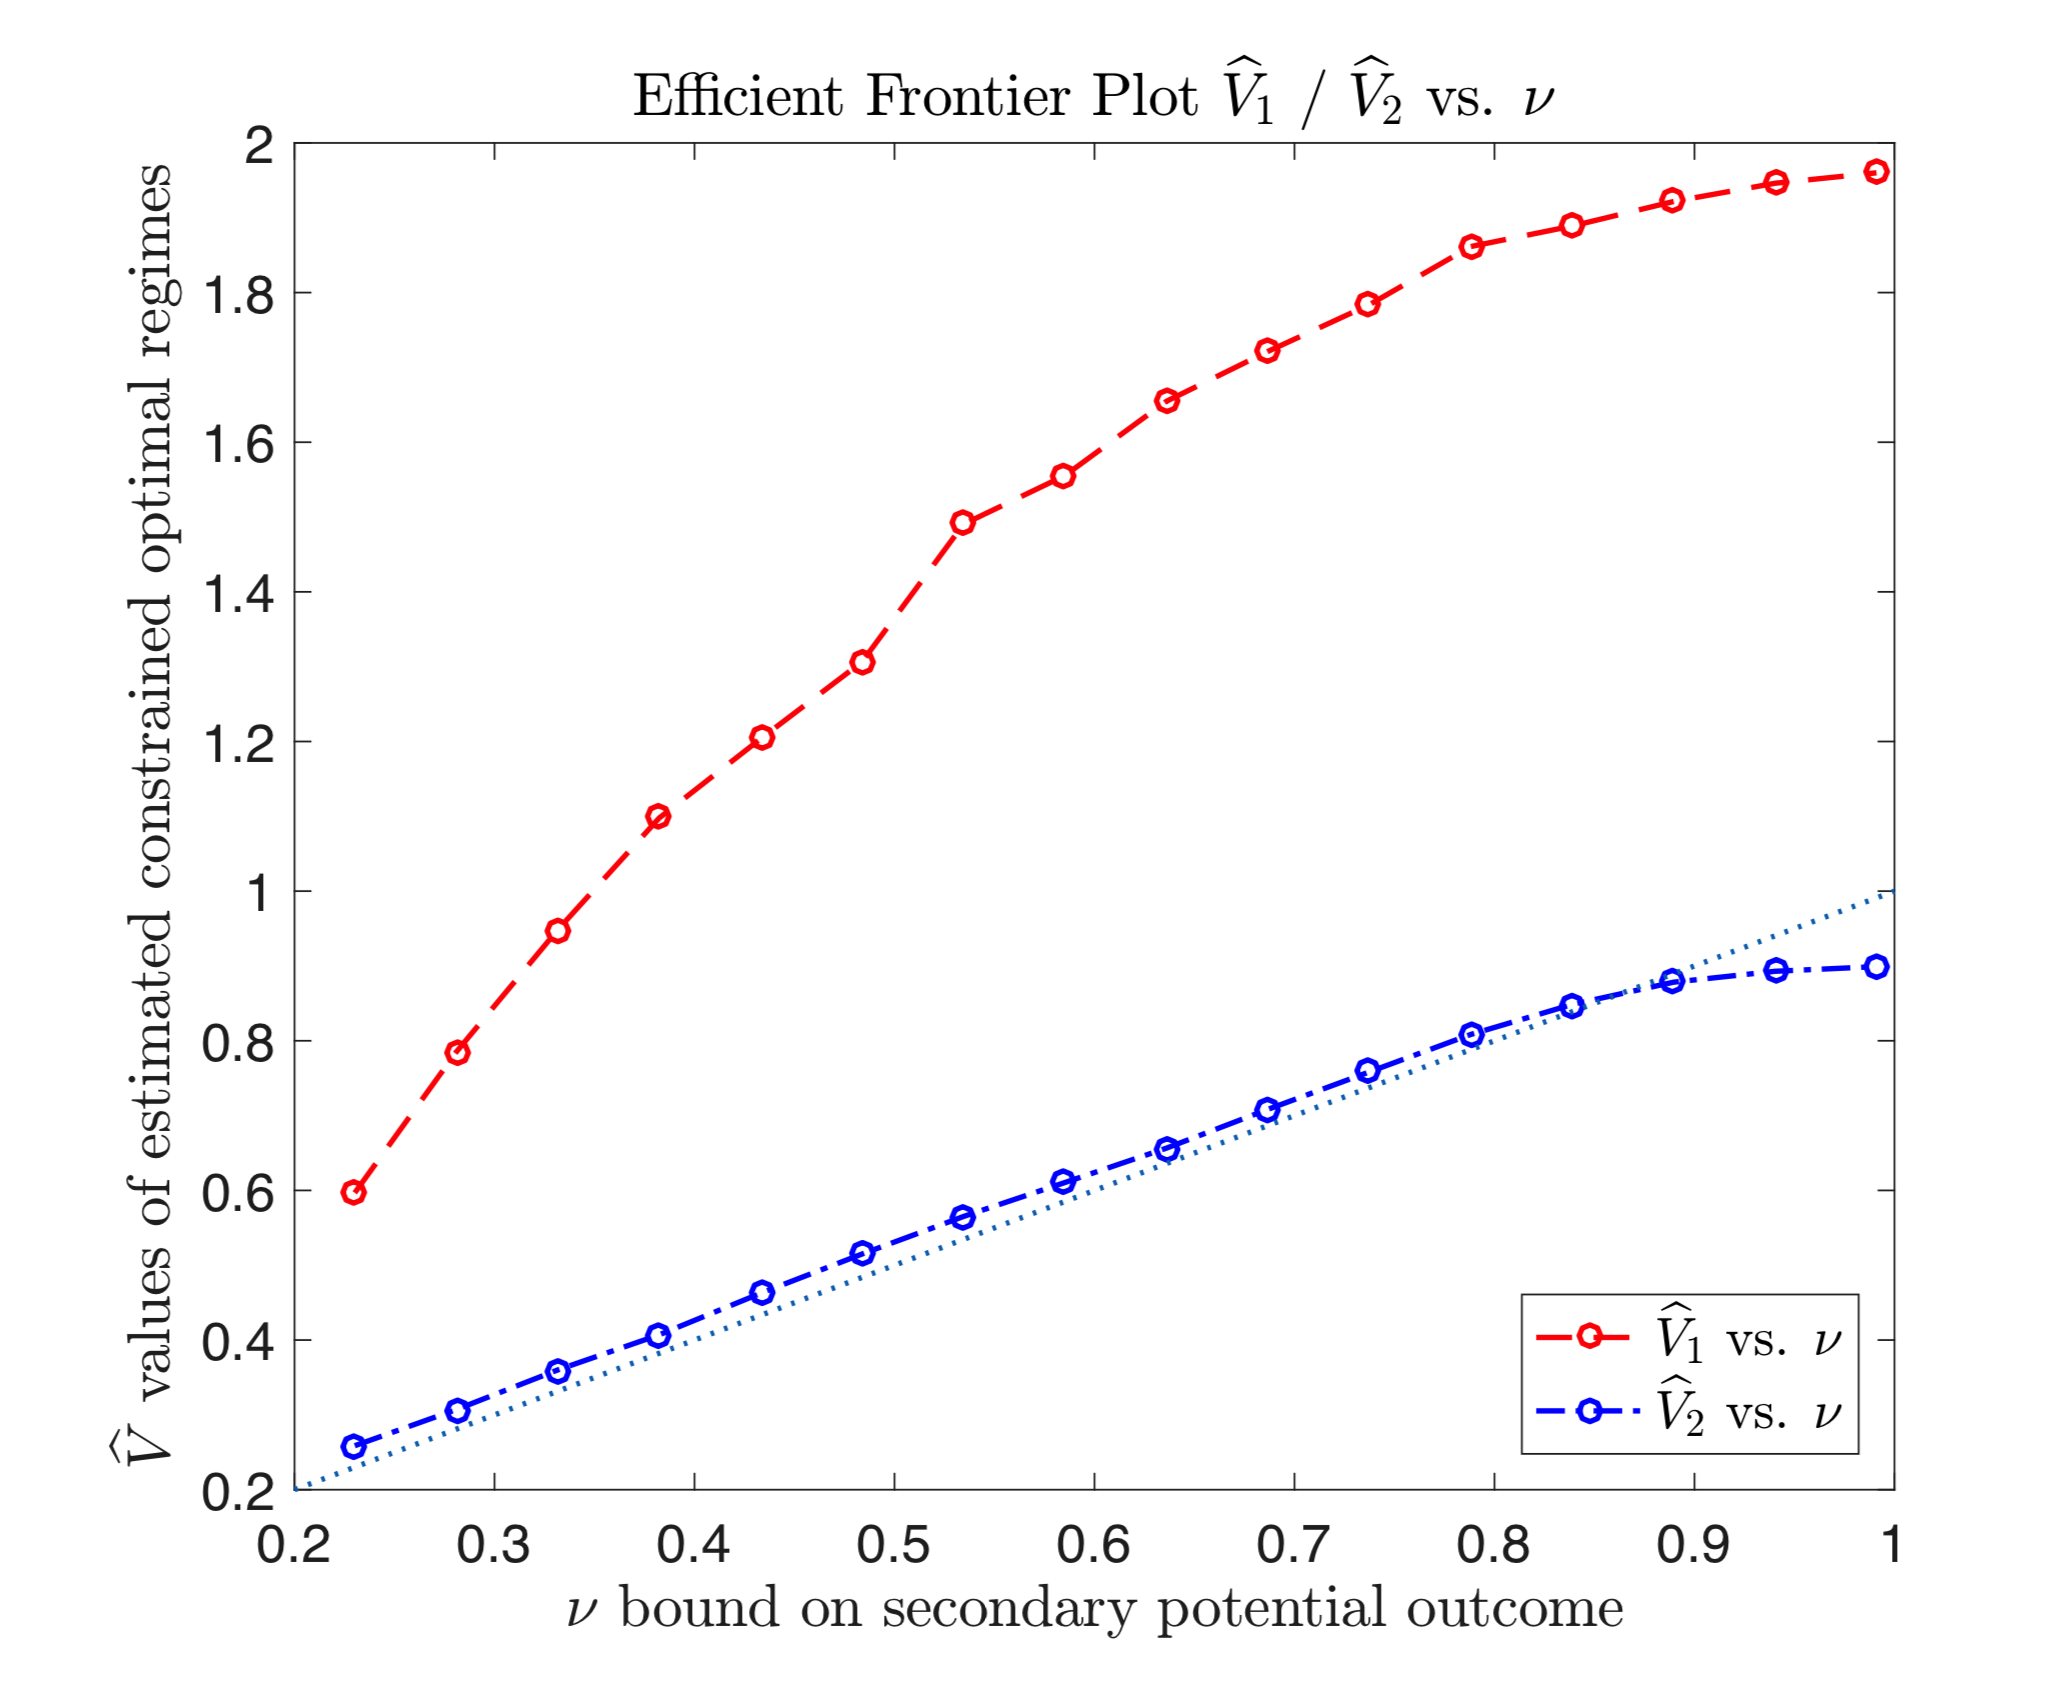
\includegraphics[width=.9\linewidth]{./figs/efficient_plot1.png}
	\caption{Efficient frontier for estimated constrained optimal regimes (single-stage) for Setting 1.}
	\label{fig:1}
\justify
X-axis is for the values for the constraints $\nu$; Y-axis is for the values of estimated regimes. Red dashed line is for the values in terms of the primary outcome of interest. Blue dashed line is for the values in terms of the secondary outcome of interest.
\end{figure}


\section{Conclusion}
Most of the research in dynamics treatment regimes has been focusing on optimizing a single scalar outcome. However, it may be an oversimplification of the goals of practical clinical decision making. In this chapter, a new method is proposed to handle multiple competing outcomes. We cast estimation of an optimal treatment regime with competing outcomes as a constrained optimization problem, which maximizes the primary outcome of interest, subject to the constraints on the secondary outcomes of interest. We prove that our estimator of a constrained optimal treatment regime is consistent under mild regularity conditions. The asymptotic limiting distribution is derived for the estimated indexing parameter for the estimated optimal regimes. Our efficient frontier plots provide an intuitive way for clinicians to examine the trade-off between multiple competing outcomes. 

\bibliography{ShupingR-thesis}{}
\bibliographystyle{plain}

\begin{appendices}
\section{Conditions for convergence of the penalty-barrier trajectory for mixed constraints}
We revisit the conditions under which the  penalty-barrier trajectory converging to the solution to the original mixed-constraint problem. The original inequality-equality constrained problem is 
\begin{align}
\begin{split}
&\underset{\bs{x} \in \mb{R}^n}{\text{minimize }}f\lt(\bs{x}\rt)\\
\text{subject to }&  c_i\lt(\bs{x}\rt) \ge 0, i\in \mathcal{I} \text{, and } c_j\lt(\bs{x}\rt) = 0, j \in \mathcal{E} ,
\end{split}
\end{align}
where $\mathcal{I}$ is the set of the indices for inequality constraints, and $\mathcal{E}$ is the set of the indices for equality constraints. Let $\bs{x}^*$ denote a solution to the original problem (A.1). A classical strategy to solve this mixed constraint problem is to find an unconstrained minimizer of a composite function that consists of the objective function, the barrier penalty for the inequality constraints, and the quadratic penalty for the equality constraints, i.e., a penalty-barrier function. It is defined as
\begin{align}
\Phi_{PB}\lt(\bs{x}, \mu \rt) \triangleq f\lt(\bs{x}\rt) - \mu \underset{ i \in \mathcal{I}}{\sum} \text{log }c_i\lt(\bs{x}\rt) + \frac{1}{2\mu} \underset{j \in \mathcal{E}}{\sum}c^2_j\lt(\bs{x}\rt),
\end{align}
where $\mu$ is a sequence of sufficiently small, positive decreasing constants. Let $\bs{x}(\mu)$ denote an unconstrained minimizer of $\Phi_{PB}(\bs{x}, \mu)$. The following theorem gives the conditions that ensure the convergence of the differentiable penalty-barrier trajectory sequence $\lt\{ \bs{x}(\mu)\rt\}$ to the original solution $\bs{x}^*$.
\begin{theorem}[Second-Order Sufficient Conditions for Problem (A.1)~\cite{fiacco, Forsgren2002}]
	Sufficient conditions that a point $\bs{x}^*$ be an isolated (uniquely) local minimum of Problem (A.1), where $f$, $c_i, \, \forall i \in \mathcal{I}$, and $c_j, \forall j \in \mathcal{E}$ are twice-differentiable functions, are that there exist vectors $\lambda_{\mathcal{I}}^*$ and $\lambda_{\mathcal{E}}^*$ such that $\lt(\bs{x}^*, \lambda_{\mathcal{I}}^*, \lambda_{\mathcal{E}}^*\rt)$ satisfies
	\begin{enumerate}
		\item $\bs{x}^*$ is feasible and the LICQ (Linear Independence Constraint Qualification) holds at $\bs{x}^*$, i.e., the Jacobian matrix of active constraints at $\bs{x}^*$, $J_{\mathcal{A}}(\bs{x}^*)$, has full row rank;
		\item $\bs{x}^*$ is a KKT point and strict complementarity holds, i.e, the (necessarily unique) multiplier $\lambda^*$ has the property that $\lambda_i^* > 0$, for all $i  \in \mathcal{A}_{\mathcal{I}}(\bs{x}^*)$, the set of indices of active inequality constraints at $\bs{x}^*$;
		\item for all nonzero vectors $p$ satisfying $J_{\mathcal{A}}(\bs{x}^*)\bs{p} = 0$, there exists $\omega > 0$ such that $\bs{p}^{\itl}H(\bs{x}^*, \lambda^*) \bs{p} \ge \omega \|\bs{p}\|^2$., where $H(\bs{x}^*, \lambda^*) $ is the hessian of the Lagrangian at $\bs{x}^*$ and $\lambda^*$.
	\end{enumerate}
\end{theorem}
\begin{theorem}[Isolated Trajectory for $\Phi_{PB}(\bs{x}, \mu)$ Function~\cite{fiacco, Forsgren2002}]
	If (a) the functions $f$, $c_i, \forall i \in \mathcal{I}$, and $c_j, \,\forall j \in \mathcal{E}$ are twice differentiable, (b) the gradients $\nabla c_i, \,\forall i \in \mathcal{I}$, and $\nabla c_j, \forall j \in \mathcal{E}$ are linearly independent, (c) strict complementarity holds for  $u_i^* c_i (\bs{x}^*) = 0, \forall i \in \mathcal{I}$, and (d) the sufficient conditions stated above under which $\bs{x}^*$ be an isolated local constrained minimum of Problem (A.1) are satisfied by $\lt(\bs{x}^*, \lambda_{\mathcal{I}}^*, \lambda_{\mathcal{E}}^*\rt)$, then there is a positive neighborhood about $\mu = 0$ for which a unique-isolated differentiable function $\bs{x}(\mu)$ exists that describes a unique isolated trajectory of local minima of $\Phi_{PB}\lt(\bs{x}, \mu\rt)$, where $\bs{x}\lt(\mu\rt) \to \bs{x}^*$ as $\mu \to 0$.
\end{theorem}
Note that $c_i\lt(\bs{x}\rt), \forall i \in \mathcal{I}$ is embedded  in the log operator, $c_i(\bs{x}_\mu)> 0$ is enforced implicitly.
\section{Proof of Theorem 1.1.2}
\begin{theorem}
	For any fixed $\mu$, assume 
	\begin{enumerate}
		\item Point-wise convergence of $\wh{v}_j(\bs{\theta})$ in probability:\\ For every $ \bs{\theta} \in \ml{F}(\bs{\Theta})$, we have $ \underset{n \to \infty}{\lim} \text{Pr} \lt\{ \mid v_j(\bs{\theta}) - \wh{v}_j(\bs{\theta}) \mid \le \epsilon_j \rt\}  = 1$, $\forall \epsilon_j > 0$, where $j = 1, \cdots, J$;
		\item Existence of a strict local minimizers of $\phi^{PB}_{\mu}\lt(\bs{\theta}\rt)$:\\
		There exists a neighborhood of $\bs{\theta}^{*}_{\bs{\nu}}(\mu)$, denoted $\ml{N}\lt(\bs{\theta}^{*}_{\bs{\nu}}(\mu)\rt)$ such that $\phi^{PB}_{\mu}\lt(\bs{\theta}^{*}_{\bs{\nu}}(\mu)\rt) < \phi^{PB}_{\mu}\lt(\bs{\theta}\rt)$, for any $\bs{\theta} \in \ml{N}\lt(\bs{\theta}^{*}_{\bs{\nu}}(\mu)\rt)$;
		\item Existence of strict local minimizer $\wh{\bs{\theta}}_{\bs{\nu}}(\mu)$ of $\wh{\phi}^{PB}_{\mu}\lt(\bs{\theta}\rt)$ in the neighborhood $\ml{N}\lt(\bs{\theta}^{*}_{\bs{\nu}}(\mu)\rt)$:\\  
		$ \wh{\phi}^{PB}_{\mu}\lt(\wh{\bs{\theta}}_{\bs{\nu}}(\mu)\rt) < \wh{\phi}^{PB}_{\mu}\lt(\bs{\theta}\rt)$, for any $\bs{\theta} \in \ml{N}\lt(\bs{\theta}^{*}_{\bs{\nu}}(\mu)\rt)$, where $\wh{\bs{\theta}}_{\bs{\nu}}(\mu) \in \ml{N}\lt(\bs{\theta}^{*}_{\bs{\nu}}(\mu)\rt)$;
	\end{enumerate} then 
	$$\wh{\bs{\theta}}_{\bs{\nu}}(\mu) \overset{p}{\to} \bs{\theta}^{*}_{\bs{\nu}}(\mu).$$
	%\begin{equation*}
	%\begin{aligned}
	%\underset{\bs{\theta} \in \ml{F}(\bs{\Theta})}{\sup} \mid \wh{\phi}^{PB}_{\mu}(\bs{\theta}) - \phi^{PB}_{\mu}(\bs{\theta})\mid = o_{p}(1).
	%\end{aligned}
	%\end{equation*}
	
	%Assume 1 - 3 in Lemma 1.1.2 hold, and then, for any fixed $\mu$,
	%\begin{equation*}
	%\begin{aligned}
	%\wh{\bs{\theta}}_{\bs{\nu}}(\mu) \overset{p}{\to} \bs{\theta}^{*}_{\bs{\nu}}(\mu).
	%\end{aligned}
	%\end{equation*}
\end{theorem}

\begin{proof}
	In this part, we simplify the notations locally just for this proof. Suppose there exists a local minimum $\bs{\theta}^{*} = \bs{\theta}^{*}_{\bs{\nu}}(\mu)$. Let its estimator be $ \wh{\bs{\theta}} = \wh{\bs{\theta}}_{\bs{\nu}}(\mu)$ and its neighborhood $\ml{N}^{*} = \ml{N}\lt(\bs{\theta}^{*}_{\bs{\nu}}(\mu)\rt)$. Also, let $\phi\lt(\bs{\theta}\rt) = \phi^{PB}_{\mu}\lt(\bs{\theta}\rt)$ and $\wh{\phi}(\bs{\theta}) = \wh{\phi}^{PB}_{\mu}\lt(\bs{\theta}\rt)$.
	By assumption 1, $\lvert \phi(\bs{\theta}^*) - \wh{\phi}(\bs{\theta}^*) \rvert = o_p(1)$, as $n \to \infty$; $\lvert \phi(\wh{\bs{\theta}}) - \wh{\phi}(\wh{\bs{\theta}}) \rvert = o_p(1)$, as $n \to \infty$. Both $\bs{\theta}^* \in \ml{N}^*$ and $\wh{\bs{\theta}} \in \ml{N}^*$ .
	\begin{flalign*} 
	\phi(\bs{\theta}^*) & = \wh{\phi}(\widehat{\bs{\theta}}) + \lt\{\phi(\bs{\theta}^*) - \wh{\phi}(\widehat{\bs{\theta}})\rt\} \\
	& > \wh{\phi}(\widehat{\bs{\theta}}) + \lt\{\phi(\bs{\theta}^*) - \wh{\phi}(\bs{\theta}^*)\rt\} \text{ (by assumption 3) }\\
	& \ge \wh{\phi}(\widehat{\bs{\theta}}) - \lvert \phi(\bs{\theta}^*) - \wh{\phi}(\bs{\theta}^*)\rvert \\
	& = \phi(\widehat{\bs{\theta}}) + \lt\{\wh{\phi}(\widehat{\bs{\theta}}) - \phi(\widehat{\bs{\theta}})\rt\}  - \lvert \phi(\bs{\theta}^*) - \wh{\phi}(\bs{\theta}^*)\rvert \\
	& \ge \phi(\widehat{\bs{\theta}}) - \lv \wh{\phi}(\widehat{\bs{\theta}}) - \phi(\widehat{\bs{\theta}})\rv - \lvert \phi(\bs{\theta}^*) - \wh{\phi}(\bs{\theta}^*)\rvert \\
	& \ge \phi(\widehat{\bs{\theta}}) + o_p(1) \text{ (implied by assumption 1) }
	\end{flalign*}
	Suppose $\wh{\bs{\theta}} \not\to \bs{\theta}^*$, and then $\phi(\bs{\theta}^*) > \liminf \phi(\wh{\bs{\theta}})$. This is opposed to assumption 2, which claims $\bs{\theta}^*$ to be a strict local minimizer. By contradictory, it is proven that $\wh{\bs{\theta}} \overset{p}{\to} \bs{\theta}^*$, as $n \to \infty$.
\end{proof}
\section{Consistency of Kernel Density Estimators}
As kernel density estimators (KDEs) are used to estimate values of regimes, we review the necessary asymptotic properties of Kernel Density Estimators briefly here.
\subsection{Consistency of univariate Kernel Density Estimator }
We review uniform consistency of Kernel Density Estimators for a univariate distribution $g(x)$ ~\cite{Silverman1978a,Pagan1999}. Consider the kernel estimate $\widehat{g}_n(x)$ of a real univariate density $g(x)$ introduced by Rosenblatt (1956) ~\cite{Silverman1978a,Pagan1999},  and defined as 
$$\widehat{g}_n(x) = \sum_{i=1}^{n} \frac{1}{nh} k\left( \frac{x-X_i}{h}\right),$$
where $X_1, \cdots, X_n$ are identically independent observations from the  distribution $g(x)$; $k$ is a kernel function satisfying suitable conditions given below; $h = h_n$ is the bandwidth which is also a function of sample size $n$.
\begin{theorem}[Uniform consistency of univariate Kernel Density Estimators]~\cite{Pagan1999,Silverman1978a}
	If all the following assumptions hold,
	\begin{enumerate}
		\item If the kernel density function $k(s)$ satisfies
		\begin{enumerate}
			\item $\int k(s)\,ds=1$;
			\item $\int \mid k(s) \mid \,ds<\infty$;
			\item $\left|s\right|\left|k(s)\right| \to 0,$ as $s \to \infty$;
			\item $\sup\left|k(s)\right|<\infty$.
			%\item $\int k^{2}(s)\,ds<\infty$.
		\end{enumerate}
		\item The bandwidth $h$ satisfies that $h \to 0$ and $nh^2 \to \infty$, as $n \to \infty$;
		\item $g(x)$ is uniformly continuous on $\mathbb{R}$;
		\item The characteristic function $\phi(t)$ of a random variable $s$ with the density $k(s)$,  $\psi(t) = \int e^{its} k(s)\,ds$, is absolutely integrable,
	\end{enumerate}
	and then we have that $\widehat{g}_n(x)$ is uniformly weak consistent, that is, 
	$$\underset{n \to \infty}{p\lim} \left[\underset{x}{\sup} \mid \widehat{g}_n(x) - g(x) \mid  \right] = 0,$$
	where $\underset{n \to \infty}{p\lim}$ denotes convergence in probability.
\end{theorem} 
\subsection{Consistency of multivariate Kernel Density Estimator }
The uniform convergence theorem of univariate Kernel Density Estimators above is extended to multivariate case by Cacoullos (1964)~\cite{Theo}. Consider an estimator of a $d$-dimensional density function $g(\boldsymbol{x})$ of the following form:
\begin{gather*}
\widehat{g}_n(\boldsymbol{x}) = \frac{1}{h^{d}} \sum_{i=1}^{n}\bar{k}\left( \frac{\boldsymbol{x} - \boldsymbol{X}_i}{h}\right)
\end{gather*}
where $\bar{k}(\boldsymbol{s})$ is a multivariate kernel of choice satisfying suitable conditions given below, and $h = h_n$ is the bandwidth. 
\begin{theorem}[Uniform consistency of multivariate Kernel Density Estimators]~\cite{Theo}
	Assume:
	\begin{enumerate}
		\item $\bar{k}(\boldsymbol{s})$ is a Borel scalar function on $\mathbb{R}^{d}$, where $\boldsymbol{s} := (s_1, \cdots, s_{d})$ such that 
		\begin{enumerate}
			\item $\idotsint \bar{k}(\boldsymbol{s}) \,ds_1\cdots \,ds_{d} = 1$;
			\item $\idotsint | \bar{k}(\boldsymbol{s}) | \,ds_1\cdots \,ds_{d}<\infty$;
			\item $|\boldsymbol{s}|^{d}|\bar{k}(\boldsymbol{s})| \to 0,$ as $\boldsymbol{s} \to \infty$, where $|\boldsymbol{s}|$ is the length of $\boldsymbol{s}$;
			\item $\underset{\boldsymbol{s}}{\sup} | \bar{k}(\boldsymbol{s}) | < \infty$.
		\end{enumerate}
		\item $h \to 0$ and $nh^{2d} \to \infty$, as $n \to \infty$;
		\item $g(\boldsymbol{x})$ is uniformly continuous in $\mathbb{R}^{d}$;
		\item The characteristic function of a random vector $\boldsymbol{s}$ with the density  of $\bar{k}(\boldsymbol{s})$, $\psi(\boldsymbol{t}) = \idotsint e^{i\boldsymbol{t}^{\intercal}\boldsymbol{s}} \bar{k}(\boldsymbol{s})\,d\boldsymbol{s}$,  is absolutely integrable,
	\end{enumerate}
	and then, $\widehat{g}_n(\boldsymbol{x})$ is uniform consistent, that is,
	\begin{gather*}
	\underset{n \to \infty}{p\lim}  \left[ \underset{\boldsymbol{x}}{\sup} \left|\widehat{g}_n(\boldsymbol{x}) - g(\boldsymbol{x}) \right| \right] = 0.
	\end{gather*}
\end{theorem}
Usually, we use a product kernel for multivariate distributions. For random vector $\boldsymbol{S}  \in \mathbb{R}^{d}$, $\boldsymbol{S} := ( S_1, \cdots, S_{d})$,
\begin{flalign*}
\frac{1}{h^{d}}\bar{k}\left(\frac{\boldsymbol{s}}{h}\right) = \frac{1}{h^{d}}\prod_{j=1}^{d}k\left(\frac{s_j}{h}\right),
\end{flalign*}
where $k(s)$ is a suitable univariate kernel function. Here, we exposit the bandwidths for each component with the same magnitude, $h_n = h$. which is also inferred by optimal bandwidth choice.
%\section{Estimating the value functions via KDE}
%We derive the value function estimator using KDE. Recall the $j$-th value function is modeled as $$V_j\lt(\bs{\theta}\rt) = m_{\bs{\alpha}^*_j}+ \iint \tsgn\lt(z_1\rt)z_2 f_{\bs{\beta}^*_j}\lt(z_1, z_2; \bs{\theta}\rt) \,dz_1 \,dz_2,$$ 
%Note, for any fixed $\bs{\beta}_j$, {\small$\iint\text{sgn}(z_1)z_2\,f_{\bs{\beta}_j}\left(z_1,z_2;\bs{\theta}\right)\,dz_1\,dz_2 =  2\iint z_2\,\mathbb{I}\left(z_1\ge0\right)\,f_{\bs{\beta}_j}\left(z_1, z_2;\bs{\theta}\right)\,dz_1\,dz_2-\int z_2\,f_{\bs{\beta}_{j}}\left(z_2\right)\,dz_2.$} To estimate this quantity, we plug in kernel density estimators for $f_{\bs{\beta}_j}(z_1, z_2; \bs{\theta})$
%and $f_{\bs{\beta}_j}( z_2 )$, and get
%
%\begin{equation}
%	\begin{aligned}
% & \iint \tsgn\lt(z_1\rt)z_2 \wh{f}_{\bs{\beta}_j}\lt(z_1, z_2; \bs{\theta}\rt) \,dz_1 \,dz_2\\
%=&2\iint z_2\,\mathbb{I}\left(z_1\ge0\right)\,\wh{f}_{\bs{\beta}_j}\left(z_1, z_2;\bs{\theta}\right)\,dz_1\,dz_2-\int z_2\,\wh{f}_{\bs{\beta}_{j}}\left(z_2\right)\,dz_2\\
%= &2\iint z_2\,\mathbb{I}\left(z_1\ge0\right)\lt\{\frac{1}{nh^2}\sum_{i=1}^{n}k\left(\frac{z_1-Z^i_1}{h}\bigg)k\bigg(\frac{z_2-Z^{i}_2}{h}\right)\rt\}\,dz_1\,dz_2-\int z_2\lt\{\frac{1}{nh}\sum_{i=1}^{n}k\left(\frac{z_2-Z^{i}_2}{h}\right)\rt\}\,dz_2\\
%=  &\frac{2}{n}\sum_{i=1}^{n}\bs{X}_{1}^{i\intercal}\bs{\beta}_{j}\left\{ 1-K\left(-\frac{\bs{X}^{i\intercal}\bs{\theta}}{h}\right)\right\} -\frac{1}{n}\sum_{i=1}^{n}\bs{X}_{1}^{i\intercal}\bs{\beta}_{j}\\
%= &\frac{1}{n}\sum_{i=1}^{n}\bs{X}_{1}^{i\intercal}\bs{\beta}_{j}\left\{ 1-2K\left(-\frac{\bs{X}^{i\intercal}\bs{\theta}}{h}\right)\right\},
%\end{aligned}
%\end{equation}
%where $K(s)$ is the corresponding CDF of the kernel function $k(s)$.The third equality is derived in the following. As we use the Gaussian kernel for $k(s)$, it satisfies the following
%\begin{enumerate}
%	\item $\int_{-\infty}^{\infty}k(s)\,ds=1$;
%	\item $k(s)>0$ for all $s$;
%	\item $k(-s)=k(s)$ for all $s$; 
%	\item The first order derivative of the kernel, $k^{\prime}(s)$, exists and is bounded. 
%\end{enumerate}
%To calculate the first term on the right hand side, let $s=\frac{z_1-Z_1^i}{h}$ and $t=\frac{z_2-Z^{i}_2}{h}$.
%Then, $z_1=Z^{i}_1+sh$ and $z_2=Z^{i}_2+th$. Also,
%$dz_1=h\,ds$ and $\,dz_2=h\,dt$. Then,
%\begin{flalign*} 
%&\frac{2}{h^2}\iint z_2\,\mathbb{I}\left(z_1\ge0\right)k\lt(\frac{z_1-Z^i_1}{h}\rt)k\lt(\frac{z_2-Z_2^{i}}{h}\rt)\,dz_1\,dz_2\\
%= & 2\iint\left(Z_2^i+th\right)\,\mathbb{I}\left(Z_1^i+sh\ge0\right)k\left(s\right)k\left(t\right)\,ds\,dt\\
%= & 2\iint Z_2^i\,\mathbb{I}\left(Z_1^i+sh\ge0\right)k\left(s\right)k\left(t\right)\,ds\,dt + 2\iint th \,\mathbb{I}\left(Z_1^i+sh\ge0\right)k\left(s\right)k\left(t\right)\,ds\,dt\\
%= &  2\int Z_2^i\,\mathbb{I}\left(s\ge -\sfrac{ Z_1^i}{h}\right)k\left(s\right)\,ds + 0 \\
%= &  2 Z_2^i \lt\{ 1 - K\lt(-\sfrac{Z_1^i}{h} \rt) \rt\} \\
%= & 2\bs{X}_{1}^{i\intercal}\bs{\beta}_{j}\left\{ 1-K\left(-\frac{\bs{X}^{i\intercal}\bs{\theta}}{h}\right)\right\},
%\end{flalign*}
%where $K\left(s\right)=\int k\left(s\right)\,ds+c$. The
%third equality holds, as $\int k(t)\,dt=1$ and $\int t\,k(t)\,dt=0$.
%The fourth equality holds as $\int\mathbb{I}\left(s\ge-\sfrac{Z_i}{h}\right)k\left(s\right)\,ds=1-\int_{-\infty}^{-\sfrac{Z^i_1}{h}}k\left(s\right)\,ds=1-K\left(-\sfrac{Z^i_1}{h}\right)$,
%where $Z^i_1=\bs{X}^{i\intercal}\bs{\theta}$ and  $Z^i_2=\bs{X}_1^{i\intercal}\bs{\beta}_j$.\\
%
%To calculate the second term on the right hand side, we derive $\frac{1}{h}\int z_2k(\frac{z_2-Z^i_2}{h})\,dz_2$ by changing variable similarly. Let $t=\frac{z_2-Z^i_2}{h}$
%,and we get $z_2=Z^i_2+th$ and $\,dz_2=h\,dt$. Then,
%\begin{flalign*}
%&\frac{1}{h}\int z_2k\left(\frac{z_2-Z^i_2}{h}\right)\,dz_2
%=  \int\left(Z^{i}_2+th\right)k\left(t\right)\,dt
%=  Z^{i}_2
%= \bs{X}_{1}^{i\intercal}\bs{\beta}_{j}.
%\end{flalign*}
%Again, the second equality holds as $\int k(t)\,dt=1$,
%and $\int t\,k(t)\,dt=0$. Together, we complete the derivation for (A.3).
%
\section{Estimating the value functions via KDE}
We derive the value function estimator using KDE. Recall the $j$-th value function is modeled as $$V_j\lt(\bs{\theta}\rt) = m_{\bs{\alpha}^*_j}+ \iint \tsgn\lt(z_1\rt)z_2 f_{\bs{\beta}^*_j}\lt(z_1, z_2; \bs{\theta}\rt) \,dz_1 \,dz_2,$$ 
Note, for any fixed $\bs{\beta}_j$, {\small$\iint\text{sgn}(z_1)z_2\,f_{\bs{\beta}_j}\left(z_1,z_2;\bs{\theta}\right)\,dz_1\,dz_2 =$\\$2\iint z_2\,\mathbb{I}\left(z_1\ge0\right)\,f_{\bs{\beta}_j}\left(z_1, z_2;\bs{\theta}\right)\,dz_1\,dz_2-\int z_2\,f_{\bs{\beta}_{j}}\left(z_2\right)\,dz_2.$} To estimate this quantity, we plug in kernel density estimators for $f_{\bs{\beta}_j}(z_1, z_2; \bs{\theta})$
and $f_{\bs{\beta}_j}( z_2 )$, and get

\begin{equation}
\begin{aligned}
& \iint \tsgn\lt(z_1\rt)z_2 \wh{f}_{\bs{\beta}_j}\lt(z_1, z_2; \bs{\theta}\rt) \,dz_1 \,dz_2\\
=&2\iint z_2\,\mathbb{I}\left(z_1\ge0\right)\,\wh{f}_{\bs{\beta}_j}\left(z_1, z_2;\bs{\theta}\right)\,dz_1\,dz_2-\int z_2\,\wh{f}_{\bs{\beta}_{j}}\left(z_2\right)\,dz_2\\
= &2\iint z_2\,\mathbb{I}\left(z_1\ge0\right)\lt\{\frac{1}{nhh}\sum_{i=1}^{n}k\left(\frac{z_1-Z^i_1}{h}\bigg)k\bigg(\frac{z_2-Z^{i}_2}{h}\right)\rt\}\,dz_1\,dz_2-\int z_2\lt\{\frac{1}{nh2}\sum_{i=1}^{n}k\left(\frac{z_2-Z^{i}_2}{h}\right)\rt\}\,dz_2\\
=  &\frac{2}{n}\sum_{i=1}^{n}\bs{X}_{1}^{i\intercal}\bs{\beta}_{j}\left\{ 1-K\left(-\frac{\bs{X}^{i\intercal}\bs{\theta}}{h}\right)\right\} -\frac{1}{n}\sum_{i=1}^{n}\bs{X}_{1}^{i\intercal}\bs{\beta}_{j}\\
= &\frac{1}{n}\sum_{i=1}^{n}\bs{X}_{1}^{i\intercal}\bs{\beta}_{j}\left\{ 1-2K\left(-\frac{\bs{X}^{i\intercal}\bs{\theta}}{h}\right)\right\},
\end{aligned}
\end{equation}
where $K(s)$ is the corresponding CDF of the kernel function $k(s)$.The third equality is derived in the following. As we use the Gaussian kernel for $k(s)$, it satisfies the following
\begin{enumerate}
	\item $\int_{-\infty}^{\infty}k(s)\,ds=1$;
	\item $k(s)>0$ for all $s$;
	\item $k(-s)=k(s)$ for all $s$; 
	\item The first order derivative of the kernel, $k^{\prime}(s)$, exists and is bounded. 
\end{enumerate}
To calculate the first term on the right hand side, let $s=\frac{z_1-Z_1^i}{h}$ and $t=\frac{z_2-Z^{i}_2}{h}$.
Then, $z_1=Z^{i}_1+sh$ and $z_2=Z^{i}_2+th$. Also,
$dz_1=h\,ds$ and $\,dz_2=h\,dt$. Then,
\begin{flalign*} 
&\frac{2}{hh}\iint z_2\,\mathbb{I}\left(z_1\ge0\right)k\lt(\frac{z_1-Z^i_1}{h}\rt)k\lt(\frac{z_2-Z_2^{i}}{h}\rt)\,dz_1\,dz_2\\
= & 2\iint\left(Z_2^i+th\right)\,\mathbb{I}\left(Z_1^i+sh\ge0\right)k\left(s\right)k\left(t\right)\,ds\,dt\\
= & 2\iint Z_2^i\,\mathbb{I}\left(Z_1^i+sh\ge0\right)k\left(s\right)k\left(t\right)\,ds\,dt + 2\iint th \,\mathbb{I}\left(Z_1^i+sh\ge0\right)k\left(s\right)k\left(t\right)\,ds\,dt\\
= &  2\int Z_2^i\,\mathbb{I}\left(s\ge -\sfrac{ Z_1^i}{h}\right)k\left(s\right)\,ds + 0 \\
= &  2 Z_2^i \lt\{ 1 - K\lt(-\sfrac{Z_1^i}{h} \rt) \rt\} \\
= & 2\bs{X}_{1}^{i\intercal}\bs{\beta}_{j}\left\{ 1-K\left(-\frac{\bs{X}^{i\intercal}\bs{\theta}}{h}\right)\right\},
\end{flalign*}
where $K\left(s\right)=\int k\left(s\right)\,ds+c$. The
third equality holds, as $\int k(t)\,dt=1$ and $\int t\,k(t)\,dt=0$.
The fourth equality holds as $\int\mathbb{I}\left(s\ge-\sfrac{Z_i}{h}\right)k\left(s\right)\,ds=1-\int_{-\infty}^{-\sfrac{Z^i_1}{h}}k\left(s\right)\,ds=1-K\left(-\sfrac{Z^i_1}{h}\right)$,
where $Z^i_1=\bs{X}^{i\intercal}\bs{\theta}$ and  $Z^i_2=\bs{X}_1^{i\intercal}\bs{\beta}_j$.\\

To calculate the second term on the right hand side, we derive $\frac{1}{h}\int z_2k(\frac{z_2-Z^i_2}{h})\,dz_2$ by changing variable similarly. Let $t=\frac{z_2-Z^i_2}{h}$
,and we get $z_2=Z^i_2+th$ and $\,dz_2=h\,dt$. Then,
\begin{flalign*}
&\frac{1}{h}\int z_2k\left(\frac{z_2-Z^i_2}{h}\right)\,dz_2
=  \int\left(Z^{i}_2+th\right)k\left(t\right)\,dt
=  Z^{i}_2
= \bs{X}_{1}^{i\intercal}\bs{\beta}_{j}.
\end{flalign*}
Again, the second equality holds as $\int k(t)\,dt=1$,
and $\int t\,k(t)\,dt=0$. Together, we complete the derivation for (A.3).
\section{Proof of Lemma 1.1.3}
\begin{lemma}
	Suppose the following conditions hold 
	\begin{enumerate}
		%	\item $\bs{X}^{\itl}\bs{\theta}$ is bounded away from 0.
		\item $\forall \bs{a} \in \mathbb{R}^p$, $\exists \,\delta > 0$ ,such that 
		\begin{enumerate}
			\item $\mathbb{E}\lt|\bs{a}^{\itl}\frac{2\bs{X}_{1}^{\itl}\bs{\beta}_j}{h}k\lt(-\frac{\bs{X}^{\itl}\bs{\theta}}{h}\rt)\bs{X}-\mu_{n}\rt|^{2+\delta} < \infty$, where $\mu_{n}=\mathbb{E}\lt\{\bs{a^{\itl}}\frac{2\bs{X}_{1}^{\itl}\bs{\beta}_{j}}{h}k\lt(-\frac{\bs{X}^{\itl}\bs{\tau}}{h}\rt)\bs{X}\rt\}$
			\item $\bs{\bs{a}^{\itl}}V\lt\{\frac{2\bs{X}^{\itl}_{1}\bs{\beta}_j}{h}k(-\frac{\bs{X}^{\itl}\bs{\theta}}{h})\bs{X}\rt\}\bs{a} ^{1+\frac{\delta}{2}}< \infty$.
		\end{enumerate}
	\end{enumerate} 
	Then, for any fixed $\bs{\theta}$ and $\bs{\beta}_j$,
	\begin{gather}
	\begin{flalign*}
	\sqrt{n}\lt(\nabla\wh{V}_j\lt(\bs{\theta}, \bs{\beta}_j\rt) -  \mb{E} \lt\{\frac{2\bs{X}_{1}^{\itl}\bs{\beta}_{j}}{h}k\lt(-\frac{\bs{X}^{\itl}\bs{\theta}}{h}\rt)\bs{X}\rt\}\rt)\overset{d}{\to}N\lt(0,AV\lt\{\frac{2\bs{X}_1^{\itl}\bs{\beta}_j}{h}k\lt(-\frac{\bs{X}^{\itl}\bs{\theta}}{h}\rt)\bs{X}\rt\}\rt),
	\end{flalign*}
	\end{gather}
	where $j = 1, \cdots, J$.
\end{lemma}
Notation $\nabla$ denotes the first-order derivatives with respect to $\bs{\theta}$. $AV$ stands for asymptotic variance. Moreover, recall that $\nabla\wh{V}_j\lt(\bs{\theta}, \bs{\beta}_j\rt)=\frac{1}{n}\sum_{i=1}^{n}\frac{2\bs{X}_{1}^{i\itl}\bs{\beta}_{j}}{h}k\lt(-\frac{\bs{X}^{i\itl}\bs{\theta}}{h}\rt)\bs{X}^{i}$.
\begin{proof}
	For any  $\bs{a} \in \mathbb{R}^p$, we let $W_{ni}=\bs{a^{\intercal}}\frac{2\bs{X}_{1}^{i\intercal}\bs{\beta}_j}{h}k\lt(-\frac{\bs{X}^{i\intercal}\bs{\theta}}{h}\rt)\bs{X}_{i}$. For each value of $n$, $w_{n1},w_{n2},\cdots,w_{nn}$ are i.i.d, and functions of the sample size $n$. This is because that $\bs{X}_{i}$ are assumed to be i.i.d., and $h$ is a function of sample
	size $n$. Then, we have
	\begin{gather*}
	\mu_{n}:=\mathbb{E}W_{ni}=\mathbb{E}\lt\{\bs{a^{\intercal}}\frac{2\bs{X}_{1}^{\intercal}\bs{\beta}_j}{h}k\lt(-\frac{\bs{X}^{\intercal}\bs{\theta}}{h}\rt)\bs{X}\rt\},
	\end{gather*}
	and 
	\begin{gather*}
	\sigma_{n}^{2}:=V(W_{ni})=\bs{\bs{a}^{\intercal}}V\lt\{\frac{2\bs{X}_{1}^{\intercal}\bs{\beta}_j}{h}k\lt(-\frac{\bs{X}^{\intercal}\bs{\theta}}{h}\rt)\bs{X}\rt\}\bs{a}.
	\end{gather*}
	
	%?????????????????????????????????????????????????????????? \\
	%??? Delta method and Taylor expansion for approximation ??? \\
	%?????????????????????????????????????????????????????????? \\
	We let $G_{ni}=W_{ni}-\mu_{\ensuremath{n}}$, and $T_{n}=\sum_{i=1}^{n}G_{ni}$. Also, we let $s_{n}^{2}=V(T_{n})=\sum_{i=1}^{n}V(G_{ni})=\sum_{i=1}^{n}\sigma_{n}^{2}=n\sigma_{n}^{2}$, where the second equality is because of independence, and the last equality is due to identicalness. Therefore, $\sfrac{T_{n}}{s_{n}}$ has mean 0, and variance 1.  If we can show $G_{ni}$ satisfying the Lyapunov condition, then
	we have
	\[
	\frac{T_{n}}{s_{n}}\overset{d}{\to}N(0,1),
	\]
	as $n \to \infty$.
	
	Now, we check the Lyapunov condition, that is,~\cite{Lindsay1995,Hunter2014}
	\begin{gather*}
	\exists\delta>0, \text{ such that } \frac{1}{s_{n}^{2+\delta}}\sum_{i=1}^{n}\mathbb{E}\mid G_{n,i}\mid^{2+\delta}\to0, \text{ as } n\to0. 
	\end{gather*}
	We define, for any $\bs{a}$, 
	\begin{gather*}
	C_1 \triangleq \mathbb{E}\lt|G_{ni}\rt|^{2+\delta}=\mathbb{E}\lt|W_{ni}-\mu_{\ensuremath{n}}\rt|^{2+\delta}=\mathbb{E}\lt|\bs{a}^{\intercal}\frac{2\bs{X}_{1}^{\intercal}\bs{\beta}_j}{h}k\lt(-\frac{\bs{X}^{\intercal}\bs{\theta}}{h}\rt)\bs{X}-\mu_{n}\rt|^{2+\delta},
	\end{gather*}
	and 
	\begin{gather*}
	C_2 \triangleq s_{n}^{2+\delta}=n^{1+\frac{\delta}{2}}\sigma_{n}^{2+\delta}=n^{1+\frac{\delta}{2}}\lt\{ \bs{\bs{a}^{\intercal}}V\lt[\frac{2\bs{X}^{\intercal}_{1}\bs{\beta}_j}{h}k\lt(-\frac{\bs{X}^{\intercal}\bs{\theta}}{h}\rt)\bs{X}\rt]\bs{a}\rt\} ^{1+\frac{\delta}{2}}.
	\end{gather*}
	Then, we have
	\begin{flalign*}
	&\frac{1}{s_{n}^{2+\delta}}\sum_{i=1}^{n}\mathbb{E}\mid G_{n,i}\mid^{2+\delta}\\
	=&\frac{n\mathbb{E}\lt|\bs{a}^{\intercal}\frac{2\bs{X}_{1}^{\intercal}\bs{\beta}_j}{h}k(-\frac{\bs{X}^{\intercal}\bs{\theta}}{h})\bs{X}-\mu_{n}\rt|^{2+\delta}}{n^{1+\frac{\delta}{2}}\lt\{ \bs{a}^{\intercal}V\lt[\frac{2\bs{X}_{1}^{\intercal}\beta}{h}k(-\frac{\bs{X}^{\intercal}\bs{\theta}}{h})\bs{X}\rt]\bs{a}\rt\} ^{1+\frac{\delta}{2}}}\\
	=&\frac{\mathbb{E}\lt|\bs{a}^{\intercal}\frac{2\bs{X}_{1}^{\intercal}\bs{\beta}_j}{h}k(-\frac{\bs{X}^{\intercal}\bs{\theta}}{h})\bs{X}-\mu_{n}\rt|^{2+\delta}}{n^{\frac{\delta}{2}}\lt\{ \bs{a}^{\intercal}V\lt[\frac{2\bs{X}^{\intercal}_{1}\bs{\beta}_j}{h}k(-\frac{\bs{X}^{\intercal}\bs{\theta}}{h})\bs{X}\rt]\bs{a}\rt\} ^{1+\frac{\delta}{2}}} \\
	=&\frac{C_{1}}{n^{\frac{\delta}{2}}C_{2}}.
	\end{flalign*}
	
	As long as $\delta>0$, for finite $C_1$ and finite $C_2$, we have $\sfrac{C_{1}}{n^{\frac{\delta}{2}}C_{2}}\to0$,
	as $n\to\infty$. This means that the Lyapunov condition is satisfied, if $\mathbb{E}\lt|G_{ni}\rt|^{2+\delta}$ and $s_{n}^{2+\delta}$ are finite. Then,  by Lyapunov Central Limit Theorem, we have
	\begin{gather*}
	\frac{T_{n}}{s_{n}}\overset{d}{\to}N(0,1).
	\end{gather*}
	
	As this hold for any arbitary non-random vector $\bs{a}\in \mathbb{R}^p$, we have, by Cramer-Wold Theorem, that
	\begin{gather*}
	\sqrt{n}\lt[\sum_{i=1}^{n}\frac{2\bs{X}_{1}^{i\intercal}\bs{\beta}_j}{h}k\lt(-\frac{\bs{X}^{i\intercal}\bs{\theta}}{h}\rt)\bs{X}_{i}-\mathbb{E}\lt\{\frac{2\bs{X}_{1}^{\intercal}\bs{\beta}_j}{h}k\lt(-\frac{\bs{X}^{\intercal}\bs{\theta}}{h}\rt)\bs{X}\rt\}\rt]\overset{d}{\to}N\lt(0,V\lt\{\frac{2\bs{X}_{1}^{\intercal}\bs{\beta}_j}{h}k\lt(-\frac{\bs{X}^{\intercal}\bs{\theta}}{h}\rt)\bs{X}\rt\}\rt),
	\end{gather*}
	as $n \to \infty$. Denote $\bs{L}_{ni}=\frac{2\bs{X}_{1}^{i\intercal}\bs{\beta}_j}{h}k\lt(-\frac{\bs{X}_{i}^{\intercal}\bs{\theta}}{h}\rt)\bs{X}^{i}$,
	then this is written as
	\begin{gather*}
	\sqrt{n}\lt(\frac{1}{n}\sum_{i=1}^{n}\bs{L}_{ni}-\mathbb{E}\bs{L}_{n1}\rt)\overset{d}{\to}N\lt(0,V\lt(\bs{L}_{n1}\rt)\rt).
	\end{gather*}
	Then, we have
	\begin{gather*}
	\frac{1/n\sum_{i=1}^{n}\bs{L}_{ni}-\mathbb{E}\bs{L}_{n1}}{[V(\bs{L}_{n1})/n]^{1/2}}\frac{[V(\bs{L}_{n1})/n]^{1/2}}{\lt[AV(\bs{L}_{n1})/n\rt]^{1/2}}\overset{d}{\to}N(0,1).
	\end{gather*}
	As  $n \to \infty$, 
	\begin{gather*}
	\frac{V(\bs{L}_{n1})^{1/2}}{AV(\bs{L}_{n1})^{1/2}}\to1,
	\end{gather*}
	then we have
	\begin{gather*}
	\frac{1/n\sum_{i=1}^{n}\bs{L}_{ni}-\mathbb{E}\bs{L}_{n1}}{[AV(\bs{L}_{n1})/n]^{1/2}}\overset{d}{\to}N(0,1),
	\end{gather*}
	i.e.,
	\begin{gather*}
	\sqrt{n}\lt[1/n\sum_{i=1}^{n}\bs{L}_{ni}-\mathbb{E}\bs{L}_{n1}\rt]\overset{d}{\to}N\lt(0,AV(\bs{L}_{n1})\rt).
	\end{gather*}
	As $\frac{1}{n}\sum_{i=1}^{n}\bs{L}_{ni} = \frac{1}{n}\sum_{i=1}^n\frac{2\bs{X}_{1}^{i\intercal}\bs{\beta}_j}{h}k\lt(-\frac{\bs{X}^{i\intercal}\bs{\theta}}{h}\rt)\bs{X}^{i} =\nabla\widehat{V}_j\lt(\bs{\theta}, \bs{\beta}_j\rt)$, we have
	\begin{gather}
	\begin{flalign*}
	\sqrt{n}\lt[\nabla\widehat{V}_j\lt(\bs{\theta}, \bs{\beta}_j\rt) -\mathbb{E}\lt\{\frac{2\bs{X}_{1}^{\intercal}\bs{\beta}_j}{h}k\lt(-\frac{\bs{X}^{\intercal}\bs{\theta}}{h}\rt)\bs{X}\rt\}\rt]\overset{d}{\to}N\lt(0,AV\lt\{\frac{2\bs{X}_1^{\intercal}\bs{\beta}_j}{h}k\lt(-\frac{\bs{X}^{\intercal}\bs{\theta}}{h}\rt)\bs{X}\rt\}\rt).
	\end{flalign*}
	\end{gather}
\end{proof}
\section{Proof of Corollary 1.1.4}
\begin{corollary}
	Suppose all the assumptions in lemma 3 hold. Also, $\wh{\bs{\theta}}_{\nu}\lt(\mu\rt)$ and $\widehat{\bs{\beta}}_{j}$ are consistent estimators of $\bs{\theta}^*_{\nu}\lt(\mu\rt)$ and $\bs{\beta}_{j}^*$, respectively. Then, 
	\begin{gather}
	\begin{flalign*}
	\sqrt{n}\lt(\nabla\wh{V}_j\lt(\bs{\theta}^*_{\nu}\lt(\mu\rt)  , \wh{\bs{\beta}}_j\rt) - \mathbb{E}\lt\{\frac{2\bs{X}_{1}^{\intercal}\bs{\beta}^*_j}{h}k\lt(-\frac{\bs{X}^{\intercal}\bs{\theta}^*_{\nu}\lt(\mu\rt)}{h}\rt)\bs{X}\rt\}\rt)\overset{d}{\to}N\lt(0,AV\lt\{\frac{2\bs{X}_1^{\itl}\bs{\beta}^*_j}{h}k\lt(-\frac{\bs{X}^{\itl}\bs{\theta}^*_{\nu}\lt(\mu\rt)}{h}\rt)\bs{X}\rt\}\rt).
	\end{flalign*}
	\end{gather}
\end{corollary}
\begin{proof} For notation simplicity, again let $\bs{\theta}^* = \bs{\theta}^*_{\nu}(\mu)$ and $\wh{\bs{\theta}} = \wh{\bs{\theta}}_{\nu}(\mu)$ here.
Write
\begin{gather*}
\begin{flalign*}
 & \nabla\wh{V}_j\lt(\bs{\theta}^* , \wh{\bs{\beta}}_j\rt) - \mathbb{E}\lt\{\frac{2\bs{X}_{1}^{\intercal}\bs{\beta}^*_j}{h}k\lt(-\frac{\bs{X}^{\intercal}\bs{\theta}^*}{h}\rt)\bs{X}\rt\} \\
=  & \lt( \nabla\wh{V}_j\lt(\bs{\theta}^* , \wh{\bs{\beta}}_j\rt) - \mathbb{E}\lt\{\frac{2\bs{X}_{1}^{\intercal}\wh{\bs{\beta}}_j}{h}k\lt(-\frac{\bs{X}^{\intercal}\bs{\theta}^*}{h}\rt)\bs{X}\rt\} \rt) + \\ & \lt( \mathbb{E}\lt\{\frac{2\bs{X}_{1}^{\intercal}\wh{\bs{\beta}}_j}{h}k\lt(-\frac{\bs{X}^{\intercal}\bs{\theta}^*}{h}\rt)\bs{X}\rt\} - \mathbb{E}\lt\{\frac{2\bs{X}_{1}^{\intercal}\bs{\beta}^*_j}{h}k\lt(-\frac{\bs{X}^{\intercal}\bs{\theta}^*}{h}\rt)\bs{X}\rt\} \rt) \\
=  & \nabla\wh{V}_j\lt(\bs{\theta}^* , \wh{\bs{\beta}}_j\rt) - \mathbb{E}\lt\{\frac{2\bs{X}_{1}^{\intercal}\wh{\bs{\beta}}_j}{h}k\lt(-\frac{\bs{X}^{\intercal}\bs{\theta}^*}{h}\rt)\bs{X}\rt\}  + o_p(1)
\end{flalign*}
\end{gather*}
For the second equality, as $\wh{\bs{\beta}}_j$is consistent, $\mathbb{E}\lt\{\frac{2\bs{X}_{1}^{\intercal}\wh{\bs{\beta}}_j}{h}k\lt(-\frac{\bs{X}^{\intercal}\bs{\theta}^*}{h}\rt)\bs{X}\rt\}$\\ $- \mathbb{E}\lt\{\frac{2\bs{X}_{1}^{\intercal}\bs{\beta}^*_j}{h}k\lt(-\frac{\bs{X}^{\intercal}\bs{\theta}^*}{h}\rt)\bs{X}\rt\} = o_p(1)$ which can be proven by Taylor expansions. Let $\bs{\theta} = \bs{\theta}^*$ and $\bs{\beta}_{j} = \wh{\bs{\beta}}_{j}$ in lemma 1.1.3, and then
\begin{gather}
\begin{flalign*}
\sqrt{n}\lt(\nabla\wh{V}_j\lt(\bs{\theta}^* , \wh{\bs{\beta}}_j\rt) - \mathbb{E}\lt\{\frac{2\bs{X}_{1}^{\intercal}\wh{\bs{\beta}}_j}{h}k\lt(-\frac{\bs{X}^{\intercal}\bs{\theta}^*}{h}\rt)\bs{X}\rt\}\rt)\overset{d}{\to}N\lt(0,AV\lt\{\frac{2\bs{X}_1^{\itl}\wh{\bs{\beta}}_j}{h}k\lt(-\frac{\bs{X}^{\itl}\bs{\theta}^*}{h}\rt)\bs{X}\rt\}\rt)
\end{flalign*}
\end{gather}
As $\widehat{\bs{\beta}}_{j}$ are consistent estimators,
\begin{gather*}
\frac{AV\lt\{\frac{2\bs{X}_1^{\itl}\widehat{\bs{\beta}}_{j}}{h}k\lt(-\frac{\bs{X}^{\itl}\bs{\theta}^*}{h}\rt)\bs{X}\rt\}}{AV\lt\{\frac{2\bs{X}_1^{\itl}\bs{\beta}^*_{j}}{h}k\lt(-\frac{\bs{X}^{\itl}\bs{\theta}^*}{h}\rt)\bs{X}\rt\}} \overset{p}{\to} 1.
\end{gather*}
Together, it is proven that
	\begin{gather}
\begin{flalign*}
\sqrt{n}\lt(\nabla\wh{V}_j\lt(\bs{\theta}^* , \wh{\bs{\beta}}_j\rt) - \mathbb{E}\lt\{\frac{2\bs{X}_{1}^{\intercal}\bs{\beta}^*_j}{h}k\lt(-\frac{\bs{X}^{\intercal}\bs{\theta}^*}{h}\rt)\bs{X}\rt\}\rt)\overset{d}{\to}N\lt(0,AV\lt\{\frac{2\bs{X}_1^{\itl}\bs{\beta}^*_j}{h}k\lt(-\frac{\bs{X}^{\itl}\bs{\theta}^*}{h}\rt)\bs{X}\rt\}\rt)
\end{flalign*}
\end{gather}
\end{proof}		

\section{Proof of Theorem 1.1.5}
\begin{theorem}
	Suppose all the assumptions in Lemma 1.1.3 and Corollary 1.1.4 hold. Then we have, as $n\to \infty$
	\begin{flalign*}
	\sqrt{n}\lt(\widehat{\bs{\theta}}_{\nu}(\mu) - \bs{\theta}_{\bs{\nu}}(\mu^*)\rt) \overset{d}{\to} N\lt(\bs{0}, \bs{\Sigma}^* \rt),
	\end{flalign*}
	where $\bs{\Sigma}^* = \bs{D}^{*-1}\bs{C}^{*}\bs{D}^{*-1}$, 
	
	\begin{flalign*}
	\sqrt{n}\lt(\widehat{\bs{\theta}}_{\nu}(\mu) - \bs{\theta}^*_{\bs{\nu}}(\mu)\rt) \overset{d}{\to} N\lt(\bs{0}, \bs{\Sigma}^* \rt),
	\end{flalign*}
	where $\bs{\Sigma}^* = \bs{D}^{*-1}\bs{C}^{*}\bs{D}^{*-1}$, \\
	$\bs{C}^* =\mathbb{E}\lt\{  \nabla v_1\lt(\bs{\theta}^*_{\bs{\nu}}(\mu)\rt)\nabla v^{\itl}_1\lt(\bs{\theta}^*_{\bs{\nu}}(\mu)\rt) \rt\} - \mathbb{E}\lt\{\nabla v_1\lt(\bs{\theta}^*_{\bs{\nu}}(\mu)\rt)\rt\} \mathbb{E}\lt\{\nabla v^{\itl}_1\lt(\bs{\theta}^*_{\bs{\nu}}(\mu)\rt)\rt\}$, and $\bs{D}^*  =  \nabla^2 \phi(\bs{\theta}^*_{\bs{\nu}}(\mu))$.
\end{theorem}

\subsection{Related Limits}
Here, we exposit the terms that are involved in deriving the limiting distribution of $\widehat{\bs{\theta}}_{\nu}\lt(\mu\rt)$. 

\subsubsection{$V_j(\bs{\theta})$ and $\wh{V}_j(\bs{\theta})$}
Recall $V_j\lt(\bs{\theta}, \bs{\alpha}_j, \bs{\beta}_j\rt) = \mb{E}\lt\{\bs{X}^{\itl}_0\bs{\alpha}_j + \tsgn\lt(\bs{X}^{\itl}\bs{\theta}\rt)\bs{X}_1^{\itl}\bs{\beta}_j \rt\}$ \\$ = m_{\bs{\alpha}_j}+ \iint \tsgn\lt(z_1\rt)z_2 f_{\bs{\beta}_j}\lt(z_1, z_2; \bs{\theta}\rt) \,dz_1 \,dz_2$, and\\
$\wh{V}_j\lt(\bs{\theta}, \bs{\alpha}_j, \bs{\beta}_j\rt)=  \frac{1}{n}\sum_{i=1}^n \lt( \bs{X}_0^{i \itl}\bs{\alpha}_j +\bs{X}_{1}^{i\intercal}\bs{\beta}_{j}\lt\{ 1-2K\left(-\frac{\bs{X}^{i\intercal}\bs{\theta}}{h}\right)\rt\}\rt)$. As stated before, due the the consistency of and the KDEs, we have $p\lim_{n\to\infty}\wh{V}_j\lt(\bs{\theta}, \bs{\alpha}_j, \bs{\beta}_j\rt)=  V_j\lt(\bs{\theta}, \bs{\alpha}_j, \bs{\beta}_j\rt)$, where $p\lim$ means converging in probability. As $\wh{\bs{\alpha}}_j$ and $\wh{\bs{\beta}}_j$ are consistent estimators of $\bs{\alpha}^*_j$ and $\bs{\beta}^*_j$, we have  $p\lim_{n\to\infty}\wh{V}_j\lt(\bs{\theta}, \wh{\bs{\alpha}}_j, \wh{\bs{\beta}}_j\rt)=  V_j\lt(\bs{\theta}, \bs{\alpha}^*_j, \bs{\beta}^*_j\rt)$. As  $\wh{V}_j\lt(\bs{\theta}, \wh{\bs{\alpha}}_j, \wh{\bs{\beta}}_j\rt)$ is denoted by $\wh{V}_j\lt(\bs{\theta}\rt)$ and $V_j\lt(\bs{\theta}, \bs{\alpha}^*_j, \bs{\beta}^*_j\rt)$ is denoted by $V_j\lt(\bs{\theta}\rt)$, we have 
\begin{flalign}
p\lim_{n\to\infty}\wh{V}_j\lt(\bs{\theta}\rt)=  V_j\lt(\bs{\theta}\rt)
\end{flalign}

\subsubsection{$\nabla V_j(\bs{\theta})$ and $\nabla\wh{V}_j(\bs{\theta})$}
The gradient of the value function with respect to $\bs{\theta}$ is \\
$\nabla V_j\lt(\bs{\theta}, \bs{\alpha}_j, \bs{\beta}_j\rt) = \frac{\partial}{\partial \bs{\theta}} \mb{E}\lt\{ \tsgn\lt(\bs{X}^{\itl}\bs{\theta}\rt)\bs{X}_1^{\itl}\bs{\beta}_j \rt\} =\frac{\partial}{\partial \bs{\theta}} \iint \tsgn\lt(z_1\rt)z_2 f_{\bs{\beta}_j}\lt(z_1, z_2; \bs{\theta}\rt) \,dz_1 \,dz_2$.
The interchangeability between integral and differentiation is assumed to hold. Then, we can write $\nabla V_j\lt(\bs{\theta}, \bs{\alpha}_j, \bs{\beta}_j\rt)
 =\frac{\partial}{\partial \bs{\theta}} \mb{E}\lt\{ \tsgn\lt(\bs{X}^{\itl}\bs{\theta}\rt)\bs{X}_1^{\itl}\bs{\beta}_j \rt\} 
=  \int_{\bs{\ml{X}}}\lt\{\frac{\partial}{\partial \bs{\theta}} \tsgn\lt( \bs{x}^{\itl}\bs{\theta}\rt)\bs{x}^{\itl}\bs{\beta}_j\rt\}f(\bs{x})\,d\bs{x}
= \int_{\bs{\ml{X}}} 2\delta\lt( \bs{x}^{\itl}\bs{\theta} \rt)\bs{x}^{\itl}\bs{\beta}_j f(\bs{x})\,d\bs{x}
= \mb{E}\lt\{ 2\delta\lt( \bs{x}^{\itl}\bs{\theta} \rt)\bs{x}^{\itl}\bs{\beta}_j\rt\},$ 
where $\delta(x) = \frac{\partial}{\partial \bs{\theta}}\tsgn(x)$ is the Dirac delta function.
Our kernel $k(x)$ is the Gaussian Kernel, where $k(x) = \sfrac{1}{\sqrt{2\pi}} \exp\lt( - \sfrac{x^2}{2}\rt)$. Then, $\frac{1}{h}k\lt(\frac{x}{h}\rt) = \frac{1}{h\sqrt{2\pi}} \exp\lt( - \frac{x^2}{2h^2}\rt)$. It is defined the Dirac delta function $\delta(x)$ to be the limit (in the sense of distributions) of the sequence of zero-centered normal distributions, i.e., $\delta(x) = \underset{h \to 0}{\lim}\sfrac{1}{h\sqrt{2\pi}} \exp\lt(-\sfrac{x^2}{2h^2}\rt) = \lim_{h \to 0}\sfrac{1}{h}k\lt(\sfrac{x}{h}\rt)$. It is an even distribution, such that $\delta(x) = \delta(-x)$.Moreover, $\nabla\wh{V}_j\lt(\bs{\theta}, \bs{\beta}_j\rt)=  \sfrac{1}{n}\sum_{i=1}^{n}\sfrac{2\bs{X}_{1}^{i\itl}\bs{\beta}_{j}}{h}k\lt(-\sfrac{\bs{X}^{i\itl}\bs{\theta}}{h}\rt)\bs{X}^{i}$. Its expectation is $\mb{E}\lt\{ \nabla\wh{V}_j\lt(\bs{\theta}, \bs{\beta}_j\rt) \rt\}=  \mb{E}\lt\{ \sfrac{2\bs{X}_{1}^{\itl}\bs{\beta}_{j}}{h}k\lt(-\sfrac{\bs{X}^{\itl}\bs{\theta}}{h}\rt)\bs{X}\rt\} = \mb{E}\lt\{2\bs{X}_{1}^{\itl}\bs{\beta}_{j}\cdot\delta\lt(\bs{X}^{\itl}\bs{\theta}\rt)\rt\}.$ This is because, as $n\to \infty$, $h \to 0$  and $nh \to \infty$, we have $\lim_{n \to \infty} \sfrac{2\bs{x}_1^{\itl}\bs{\beta}_{j}}{h}k\lt(-\sfrac{\bs{x}^{\itl}\bs{\theta}}{h}\rt) = 2\bs{x}_{1}^{\itl}\bs{\beta}_{j}\cdot\delta\lt(-\bs{x}^{\itl}\bs{\theta}\rt)= 2\bs{x}_{1}^{\itl}\bs{\beta}_{j}\cdot\delta\lt(\bs{x}^{\itl}\bs{\theta}\rt)$. Thus, by weak law of large numbers, $p\lim_{n\to\infty}\nabla\wh{V}_j\lt(\bs{\theta}, \bs{\alpha}_j, \bs{\beta}_j\rt)$ \\$=\nabla V_j\lt(\bs{\theta}, \bs{\alpha}_j, \bs{\beta}_j\rt)$. Together, with the consistency of $\wh{\bs{\alpha}}_j$ and $\wh{\bs{\beta}}_j$, we have \\$p\lim_{n\to\infty}\nabla\wh{V}_j\lt(\bs{\theta},\wh{\bs{\alpha}}_j, \wh{\bs{\beta}}_j\rt)=  \nabla V_j\lt(\bs{\theta}, \bs{\alpha}^*_j, \bs{\beta}^*_j\rt)$. Using the simplified notation, that is 
\begin{flalign}
p\lim_{n\to\infty}\nabla\wh{V}_j\lt(\bs{\theta}\rt)=  \nabla V_j\lt(\bs{\theta}\rt)
\end{flalign}

\subsubsection{$\nabla^2 V_j(\bs{\theta})$ and $\nabla^2\wh{V}_j(\bs{\theta})$}
The second order derivative of value function, or Hessian, is\\
 $\nabla^2 V_j\lt(\bs{\theta}, \bs{\alpha}_j, \bs{\beta}_j\rt) = \nabla^2\mb{E}\lt\{ \tsgn\lt(\bs{X}^{\itl}\bs{\theta}\rt)\bs{X}_1^{\itl}\bs{\beta}_j \rt\} =\frac{\partial^2}{\partial \bs{\theta}\partial \bs{\theta}^{\itl}} \iint \tsgn\lt(z_1\rt)z_2 f_{\bs{\beta}_j}\lt(z_1, z_2; \bs{\theta}\rt) \,dz_1 \,dz_2$. Again, the interchangeability between integral and differentiation is assumed to hold.
 $\nabla^2\mathbb{E}\{ \text{sgn}(\bs{X}^{\itl}\bs{\theta})\bs{X}_1^{\itl}\bs{\beta}_{j}\}
=  \int_{\bs{\ml{X}}}\lt\{\frac{\partial^2}{\partial\bs{\theta}\partial\bs{\theta}^{\itl}}\tsgn\lt(\bs{x}^{\itl}\bs{\theta}\rt)\bs{x}_1^{\itl}\bs{\beta}_{j}\rt\}f\lt(\bs{x}\rt)\,d\bs{x}\\
= \int_{\bs{\ml{X}}}2\bs{x}_1^{\itl}\bs{\beta}_{j}\delta^{\prime}\lt(\bs{x}^{\itl}\bs{\theta}\rt)\bs{x}\bs{x}^{\itl}f(\bs{x})\,d\bs{x}
= \mathbb{E}\lt\{ 2\bs{X}_1^{\itl}\bs{\beta}_{j}\delta^{\prime}\lt(\bs{X}^{\itl}\bs{\theta}\rt)\bs{X}\bs{X}^{\itl}\rt\}$, where $\delta^{\prime}(x)$ is the distributional derivative of the Dirac function.  $\delta^{\prime}(x) = \lim_{h\to0} \sfrac{1}{h^2}k^{\prime}\lt(\frac{x}{h}\rt)$\\$ =  \lim_{h \to 0}  \sfrac{-x}{h^3\sqrt{2\pi}} \exp\lt( - \sfrac{x^2}{2h^2}\rt)$. Moreover, \\$ \nabla^2\wh{V}_j\lt(\bs{\theta}, \bs{\beta}_j\rt) 
=\sfrac{1}{n}\sum_{i=1}^n\lt\{-\sfrac{2\bs{X}_{1}^{i\itl}\bs{\beta}_{j}}{h^2}k^{\prime}\lt(-\sfrac{\bs{X}^{i\itl}\bs{\theta}}{h}\rt)\bs{X}^i\bs{X}^{i\itl}\rt\}$. Its expectation is\\
 $\mb{E}\lt\{ \nabla^2\wh{V}_j\lt(\bs{\theta}, \bs{\beta}_j\rt) \rt\}
=\mb{E}\lt\{-\sfrac{2\bs{X}_{1}^{\itl}\bs{\beta}_{j}}{h^2}k^{\prime}\lt(-\sfrac{\bs{X}^{\itl}\bs{\theta}}{h}\rt)\bs{X}\bs{X}^{\itl}\rt\}=\mathbb{E}\lt\{ 2\bs{X}_1^{\itl}\bs{\beta}_{j}\delta^{\prime}\lt(\bs{X}^{\itl}\bs{\theta}\rt)\bs{X}\bs{X}^{\itl}\rt\}.$ Thus, by weak law of large numbers, $p\lim_{n \to \infty}\nabla^2\wh{V}_j\lt(\bs{\theta}, \bs{\beta}_j\rt)= \nabla^2V_j\lt(\bs{\theta}, \bs{\beta}_j\rt)$. Together, with the consistency of $\wh{\bs{\beta}}_j$, $p\lim_{n \to \infty}\nabla^2\wh{V}_j\lt(\bs{\theta}, \wh{\bs{\beta}}_j\rt) =  \nabla^2V_j\lt(\bs{\theta}, \bs{\beta}^*_j\rt)$. Using simplified notation, we have 
 \begin{flalign}
 p\lim_{n \to \infty}\nabla^2\wh{V}_j\lt(\bs{\theta}\rt) =  \nabla^2V_j\lt(\bs{\theta}\rt)
 \end{flalign}

\subsection{Proof}
%\subsection{Limiting distribution of $\widehat{\bs{\tau}}_{\kappa,\mu}$}
We derive the limiting distribution of $\widehat{\bs{\theta}}_{\nu}(\mu)$, and prove Theorem 1.1.5.
\begin{proof} For notation simplicity in this proof, let $\phi\lt(\bs{\theta}\rt) = \phi^{PB}_{\mu}\lt(\bs{\theta}\rt)$ and $\wh{\phi}(\bs{\theta}) = \wh{\phi}^{PB}_{\mu}\lt(\bs{\theta}\rt)$ for this proof. Also, let $\bs{\theta}^* = \bs{\theta}^*_{\nu}(\mu)$ and $\wh{\bs{\theta}} = \wh{\bs{\theta}}_{\nu}(\mu)$ here.
Recall $\wh{\phi}\lt(\bs{\theta}\rt) = \,\,\wh{v}_1(\bs{\theta}) - \mu \sum_{j=2}^J \ln \wh{v}_j\lt( \bs{\theta}\rt) + \sfrac{1}{2\mu} \lt(\bs{\theta}^{\itl}\bs{\theta} - 1\rt)^2$.  As  $\bs{\theta}^{\itl}\bs{\theta}-1=0$ is always satisfied as a constraint, the gradient is $\nabla\wh{\phi}\lt(\bs{\theta}\rt) = \,\,\nabla\wh{v}_1(\bs{\theta}) - \mu \sum_{j=2}^J \sfrac{\nabla\wh{v}_j\lt( \bs{\theta}\rt)}{\wh{v}_j\lt( \bs{\theta}\rt)}$. Taylor expansion of $\nabla\wh{\phi}\lt(\bs{\theta}^*\rt)$ at $\bs{\theta} = \widehat{\bs{\theta}}$ shows that
	\begin{flalign*}
	\nabla\wh{\phi}\lt(\bs{\theta}^*\rt) =  \nabla\wh{\phi}(\wh{\bs{\theta}})- \nabla^2\wh{\phi}(\tilde{\bs{\theta}}) (\widehat{\bs{\theta}} - \bs{\theta}^{*}) + o_p(1),
	\end{flalign*}
	where $\tilde{\bs{\theta}}$ is between $\wh{\bs{\theta}}$ and $\bs{\theta}^*$. As $\widehat{\bs{\theta}}$ is the maximizer of $\widehat{\phi}\lt(\bs{\theta}\rt)$, it satisfies the first order condition that $\nabla \wh{\phi}(\widehat{\bs{\theta}}) = 0$. Therefore, 
	\begin{flalign}
	\sqrt{n}\nabla\wh{\phi}\lt(\bs{\theta}^*\rt) =   - \sqrt{n} \nabla^2\wh{\phi}( \tilde{\bs{\theta}}) (\widehat{\bs{\theta}} - \bs{\theta}^{*}),
	\end{flalign}
 where $\nabla\wh{\phi}\lt(\bs{\theta}\rt) = \,\,\nabla\wh{v}_1(\bs{\theta}) - \mu \sum_{j=2}^J \sfrac{\nabla\wh{v}_j\lt( \bs{\theta}\rt)}{\wh{v}_j\lt( \bs{\theta}\rt)}$.
 Recall $v_1\lt(\bs{\theta}\rt)=- V_1\lt(\bs{\theta}\rt)$ and  $v_j\lt(\bs{\theta}\rt) = V_j\lt(\bs{\theta}\rt) - \nu_j$, for $j = 2, \cdots, J$.  Due to Corollary 1.1.4, together with (A.4) and (A.5),
\begin{flalign}
\sqrt{n}\bigg(\nabla\wh{v}_1(\bs{\theta}^*) - \nabla v_1(\bs{\theta}^*)\bigg)\overset{d}{\to}N\lt( 0, \bs{C}^*\rt),
\end{flalign}

where $\bs{C}^*=AV\bigg(\nabla v_1(\bs{\theta}^*)\bigg) = AV\lt\{\frac{2\bs{X}_1^{\itl}\bs{\beta}^*_1}{h}k\lt(-\frac{\bs{X}^{\itl}\bs{\theta}^*}{h}\rt)\bs{X}\rt\}$. That is,
 \begin{gather*}
\begin{flalign*}
\bs{C}^* \triangleq =&AV\bigg(\nabla v_1(\bs{\theta}^*)\bigg)=
AV\lt[\frac{2\bs{X}_1^{\itl}\bs{\beta}^*_{1}}{h}k\lt(-\frac{\bs{X}^{\itl}\bs{\theta}^*}{h}\rt)\bs{X} \rt] = p\lim_{n \to \infty} V\lt[\frac{2\bs{X}_1^{\itl}\bs{\beta}^*_{1}}{h}k\lt(-\frac{\bs{X}^{\itl}\bs{\theta}^*}{h}\rt)\bs{X} \rt] \\
= & p\underset{n \to \infty}\lim \lt[ \mathbb{E} \lt\{ \frac{4\bs{\beta}^{*\itl}_{1}\bs{X}_1\bs{X}_1^{\itl}\bs{\beta}^*_{1}}{h^2}k^2\lt(-\frac{\bs{X}^{\itl}\bs{\theta}^*}{h}\rt)\bs{X}\bs{X}^{\itl}\rt\} -  \mathbb{E}\lt\{\frac{2\bs{X}_1^{\itl}\bs{\beta}^*_{1}}{h}k\lt(-\frac{\bs{X}^{\itl}\bs{\theta}^*}{h}\rt)\bs{X}\rt\} \mathbb{E}\lt\{\frac{2\bs{X}_1^{\itl}\bs{\beta}^*_{1}}{h}k\lt(-\frac{\bs{X}^{\itl}\bs{\theta}^*}{h}\rt)\bs{X}\rt\}^{\itl} \rt] \\
= & \mathbb{E}\lt\{  4\big(\bs{X}_1^{\itl}\bs{\beta}^*_{1}\delta\lt(\bs{X}^{\itl}\bs{\theta}^*\rt)\big)^2\bs{X}\bs{X}^{\itl} \rt\} - \mathbb{E}\lt\{2\bs{X}_1^{\itl}\bs{\beta}^*_{1}\delta\lt(\bs{X}^{\itl}\bs{\theta}^*\rt)\bs{X}\rt\} \mathbb{E}\lt\{2\bs{X}_1^{\itl}\bs{\beta}^*_{1}\delta\lt(\bs{X}^{\itl}\bs{\theta}^*\rt)\bs{X}\rt\}^{\itl}\\
=& \mathbb{E}\lt\{  \nabla v_1(\bs{\theta}^*)\nabla^{\itl} v_1(\bs{\theta}^*) \rt\} - \mathbb{E}\lt\{\nabla v_1(\bs{\theta}^*)\rt\} \mathbb{E}\lt\{\nabla^{\itl} v_1(\bs{\theta}^*)\rt\}.
\end{flalign*}
\end{gather*}
Then, due to (A.4) and (A.5), we have
\begin{flalign}
\sum_{j=2}^J \frac{\nabla\wh{v}_j\lt( \bs{\theta}\rt)}{\wh{v}_j\lt( \bs{\theta}\rt)} -  \sum_{i=2}^{J}\frac{\nabla v_j(\bs{\theta})}{v_j(\bs{\theta})} = o_p(1).
\end{flalign}
Note $v_j(\bs{\theta}) > 0$, for $j =2, \cdots, J$, is implied by the log barrier operator. Put (A.8) and (A.9) together by Slutsky's theorem, we have
\begin{flalign*}
\sqrt{n}\lt\{\lt(\nabla\wh{v}_1(\bs{\theta}^*) - \mu \sum_{j=2}^J \frac{\nabla\wh{v}_j\lt( \bs{\theta}^*\rt)}{\wh{v}_j( \bs{\theta}^*)}\rt) - \lt(\nabla v_1(\bs{\theta}^*) - \mu \sum_{i=2}^{J}\frac{\nabla v_j(\bs{\theta}^*)}{v_j(\bs{\theta}^*)}\rt)\rt\}\overset{d}{\to}N\lt(0, \bs{C}^*\rt),
\end{flalign*} 
Due to the stationarity of $\bs{\theta}^*$, $\nabla \phi(\bs{\theta}^*)=\nabla v_1(\bs{\theta}^*) - \mu \sum_{i=2}^{J}\sfrac{\nabla v_j(\bs{\theta}^*)}{v_j(\bs{\theta}^*)} =0$. Together with Sluskty's theorem, we have 
\begin{flalign*}
\sqrt{n} \nabla\wh{\phi}( \bs{\theta}^*) \overset{d}{\to} N\lt(0, \bs{C}^*\rt),
\end{flalign*}
where 
$\bs{C}^* =\mathbb{E}\lt\{  \nabla v_1(\bs{\theta}^*)\nabla^{\itl} v_1(\bs{\theta}^*) \rt\} - \mathbb{E}\lt\{\nabla v_1(\bs{\theta}^*)\rt\} \mathbb{E}\lt\{\nabla^{\itl} v_1(\bs{\theta}^*)\rt\}.$ \\

As $	\sqrt{n}\nabla\wh{\phi}\lt(\bs{\theta}^*\rt) =  - \sqrt{n} \nabla^2\wh{\phi}( \tilde{\bs{\theta}}) (\widehat{\bs{\theta}} - \bs{\theta}^{*})$ stated in (A.7),we have
\begin{flalign}
\sqrt{n} \nabla^2\wh{\phi}( \tilde{\bs{\theta}}) (\widehat{\bs{\theta}} - \bs{\theta}^{*}) \overset{d}{\to} N(0, \bs{C}^*)
\end{flalign} 	
The Hessian is $\nabla^2\wh{\phi}\lt(\bs{\theta}\rt) = \,\,\nabla^2\wh{v}_1(\bs{\theta}) - \mu \sum_{j=2}^J \sfrac{\big(\nabla^2\wh{v}_j\lt( \bs{\theta}\rt)\wh{v}_j\lt( \bs{\theta}\rt)- \lt(\nabla\wh{v}_j\lt( \bs{\theta}\rt)\rt)^2\big)}{\wh{v}^2_j\lt( \bs{\theta}\rt)}$. Based on (A.4) and (A.5), we have
\begin{gather}
\begin{flalign}
\bs{D}^* \triangleq & p\lim_{n \to \infty}\nabla^2\wh{\phi}\lt(\bs{\theta}^*\rt) =  \nabla^2 \phi(\bs{\theta}^*)
 =\nabla^2{v}_1(\bs{\theta}^*) - \mu \sum_{j=2}^J \frac{\nabla^2{v}_j\lt( \bs{\theta}^*\rt)v_j\lt( \bs{\theta}^*\rt)- \lt\{\nabla v_j\lt( \bs{\theta}^*\rt)\rt\}^2}{v^2_j\lt( \bs{\theta}^*\rt)}.
\end{flalign}
 \end{gather}

As $\tilde{\bs{\theta}}$ is a vector in-between $\bs{\theta}^*$ and $\wh{\bs{\theta}}$, we have $\nabla^2\wh{\phi}(\tilde{\bs{\theta}}) = \nabla^2\wh{\phi}(\bs{\theta}^*) + o_p(1)$. Therefore, based on (A.10) and (A.11), we have 
\begin{flalign*}
\sqrt{n}\lt(\widehat{\bs{\theta}} - \bs{\theta}^*\rt) \overset{d}{\to} N\lt(\bs{0}, \bs{\Sigma}^* \rt),
\end{flalign*}
where $\bs{\Sigma}^* = \bs{D}^{*-1}\bs{C}^{*}\bs{D}^{*-1}$, 
$\bs{C}^* =\mathbb{E}\lt\{  \nabla v_1(\bs{\theta}^*)\nabla^{\itl} v_1(\bs{\theta}^*) \rt\} - \mathbb{E}\nabla v_1(\bs{\theta}^*) \mathbb{E}\nabla^{\itl} v_1(\bs{\theta}^*)$ and $\bs{D}^*  =  \nabla^2 \phi(\bs{\theta}^*)$.
\end{proof}
%\begin{section}{Proof of Theorem 1.1.6}
%	\begin{theorem}
%		Suppose all the assumptions in Theorem 1.1.5 hold, then $$\wh{V}_j(\wh{\bs{\theta}}_{\bs{\nu}}(\mu)) - V_j(\bs{\theta}_{\bs{\nu}}^*(\mu))\overset{d}{\to} N\lt\{0, \nabla^{\itl} V_j\lt(\bs{\theta}^*_{\bs{\nu}}(\mu)\rt) \bs{\Sigma}^*\nabla V_j\lt(\bs{\theta}^*_{\bs{\nu}}(\mu)\rt)\rt\}.$$
%	\end{theorem}
%	\begin{proof}
%Again, for notation simplicity, let $\bs{\theta}^* = \bs{\theta}^*_{\bs{\nu}}(\mu)$ and $\wh{\bs{\theta}} = \wh{\bs{\theta}}_{\bs{\nu}}(\mu)$ for this proof. We write
%	\begin{flalign*}
%	 & \wh{V}_j(\wh{\bs{\theta}}) - V_j(\bs{\theta}^*) \\
%  = & \,\wh{V}_j(\wh{\bs{\theta}}) - \wh{V}_j(\bs{\theta}^*) + \wh{V}_j(\bs{\theta}^*) - V_j(\bs{\theta}^*) \\
%  = & \,\wh{V}_j(\wh{\bs{\theta}}) - \wh{V}_j(\bs{\theta}^*)  + o_p(1) \,\,\, \text{by (A.4)} \\
% = & \nabla \wh{V}_j(\tilde{\bs{\theta}}) ( \wh{\bs{\theta}} - \bs{\theta}^*) + o_p(1) \,\,\, \text{by Taylor expansion} \\
% = & \nabla V_j(\bs{\theta}^*) ( \wh{\bs{\theta}} - \bs{\theta}^*) + o_p(1) 
%\end{flalign*}
%For last equality, by (A.5), $\nabla \wh{V}_j(\tilde{\bs{\theta}}) \overset{p}{\to} \nabla V_j(\tilde{\bs{\theta}})$; as $\tilde{\bs{\theta}}$ is in-between $\wh{\bs{\theta}}$ and $\bs{\theta}^*$ and $\wh{\bs{\theta}} - \bs{\theta}^* = o_p(1)$, $\nabla \wh{V}_j(\tilde{\bs{\theta}}) \overset{p}{\to} \nabla V_j(\bs{\theta}^*)$. By Theorem 1.1.5, $\sqrt{n}(\wh{\bs{\theta}} - \bs{\theta}^*) \overset{d}{\to} N(0, \bs{\Sigma}^*)$. Thus, $\nabla V_j(\bs{\theta}^*) ( \wh{\bs{\theta}} - \bs{\theta}^*)\overset{d}{\to} N(0, \nabla^{\itl} V_j(\bs{\theta}^*) \bs{\Sigma}^*\nabla V_j(\bs{\theta}^*) )$.
%	\end{proof}
%
%	\end{section}
\section{Details on simulation }
\subsection{Parameters}
	To find parameter values in the generative model that satisfy the levels of these two factors, we use the solver \texttt{fmincon} in Matlab to minimize the sum of two empirical quadratic loss functions for $\Omega_1$ and $\Omega_2$ and find a set of possible solution. \\
	\subsection{Details about simulation studies with kernel density estimation}
%	For each setting, the simulation followed the steps below.
%	\begin{enumerate} 
%		\item The training dataset $\{(H_{i}, A_{i}, Y_{i}, Z_{i})\}^{n}_{i=1}$ is generated according to the generative model above using each set of the parameters in Table 2.
%		\item We to estimate the parameters, $\bs{\alpha}^*_1$, $\bs{\beta}^*_1$, $\beta^{*}_{0Z}$ and $\beta^{*}_{1Z}$ using least-squares based on the training dataset and denote the estimators $\hat{\beta}_{0Y}$, $\hat{\beta}_{1Y}$, $\hat{\beta}_{0Z}$ and $\hat{\beta}_{1Z}$.
%		\item For any $\tau : \|\tau\|=1$, the density of $(H^{\itl}\beta_{1Y}^{*}, H^{\itl}\tau)$ is estimated using a bivariate kernel density estimator with data points $(H^{\itl}\hat{\beta}_{1Y}, H^{\itl}\tau)$ from the training dataset. Then, we use the sample mean from the estimated density to approximate $E \{sgn(\bs{X}^{\itl}\tau) H_{1}^{\itl}\bs{\beta}^*_1 \}$. A similar approach is used to estimate $E \{sgn(\bs{X}^{\itl}\tau) H^{\itl}\beta^{*}_{1Z} \}$. $E\{H^{\itl}_{0}\beta^{*}_{0Z}\}$ is approximated by $\hat{E}(H^{\itl}_{0}\hat{\beta}_{0Z}) =n^{-1}\sum_{i=1}^{n} \bs{X}^{\itl}_{0i}\hat{\beta}_{0Z}$, where n is the sample size of the training data. 
%		\item For a sequence of upper bounds
%		on $E \{Z^{*}(\pi)\}$, $\kappa_{j}$, $j = 1, . . . , J$, we solve the constrained optimization problem formed in step 3 using the log barrier or exact penalty method and get the estimates $\hat{\tau}_{n,\kappa}$. 
%		\item A testing dataset is generated from the same model. We apply the estimated constrained optimal regime $\hat{\pi}_{opt,\kappa}$ to the test dataset and calculate $\hat{E}\{Y^{*}(\hat{\pi}_{opt,\kappa})\} = m^{-1}{\sum_{i=1}^{m} Y^{*}_{i}\{\hat{\pi}_{opt,\kappa}(h_i)\}}$, the sample means of Y under the estimated optimal constrained regime, where $m$ is the sample size of the test dataset. Then, we plot $\hat{E}\{Y^{*}(\hat{\pi}_{opt,\kappa})\}$ v.s. $\kappa$,
%		along with a $95\%$ point-wise confidence interval.
%	\end{enumerate}
%	
%	In our simulations, the training dataset sample size $n$ is chosen to be 1,000 and the test dataset sample size $m$ is set to be 1,000 as well. The number of Monte Carlo replicates is 200. A Matlab nonlinear optimization solver, fminsearch, is used to solve the functions for both log barrier and exact penalty functions. Fimsearch uses the simplex search method of Lagarias et al~\cite{JeffreyC.Lagarias}. It can often handle discontinuity, particularly if it does not occur near the solution, but is only guaranteed to find local optimum~\cite{JeffreyC.Lagarias, MATLAB}. For the log barrier method, we follow the suggestion by Linn et al.~\cite{Linn2014} and set a sequence of decreasing $\lambda_{1} > \lambda_{2} > ... > \lambda_{K}$ with $\lambda_{j} = \lambda_{j-1}/4$.  The solution for $\tau$ at $\lambda_{j-1}$ is used as the starting value for $\tau$ at $\lambda_j$. We choose $\lambda_1$ so that $$\hat{E}\{Y^{*}(\hat{\pi}_{Y, opt})\} - \hat{E}(Y) = \lambda_{1} log \big[ \kappa - \hat{E}\{Z^{*}(\hat{\pi}_{Z, opt})\} \big],$$
%	By doing so, the log-penalty should have the same order of magnitude as the potential gain in the mean of Y over treatment randomization~\cite{Linn2014}. At $\lambda_1$ , the starting value for $\tau$ is $\hat{\tau}_{n,Z} = \underset{\tau: \| \tau\| =1}{\text{argmin }}\hat{E}_{H} {\lt\{H^{\itl}\hat{\beta}_{0Z} + sgn(\bs{X}^{\itl}\tau) H^{\itl}\hat{\beta}_{1Z} \rt\} }$, which is the estimated indexing parameter for the optimal regime in terms of $Z$. For exact penalty method, $\lambda$ is set to be 3000. We used 10 random starts used for solving the exact penalty function. Kernel Density Estimation Toolbox for MATLAB is used~\cite{matlabKDE}. The kernel is chosen to be the 2 dimensional Gaussian kernel. Silverman's rule of thumb is used to decide the bandwidth~\cite{nonparm}. In the plots, the means of Y under the true optimal constrained regimes $\hat{E}\{Y^{*}(\pi^{*}_{opt,\kappa})\}$ vs $\kappa$ are also included. Here, $\pi^{*}_{opt,\kappa}$ is obtained by solving the constrained optimization problem with true parameters $\bs{\beta}^*_1$, $\beta^{*}_{0Z}$ and $\beta^{*}_{1Z}$ in the functions using one set of training data with sample size 10,000. Both log barrier and exact penalty methods are carried out. $\hat{E}\{Y^{*}(\pi^{*}_{opt,\kappa})\} = m^{-1}{\sum_{i=1}^{m} Y^{*}_{i}\{\pi^{*}_{opt,\kappa}(h_i)\}}$  is obtained by applying the true constrained optimal regime to one set of testing data with sample size 10,000. 
	\subsection{Simulation results}

\begin{table}[!htbp]
	\caption {Simulation Result for Setting 2}
	\centering
	{\tt
		\begin{tabular}{rrrrrrrrrr}\hline 
setting & $\nu$  & $\wh{V}_1(\wh{\bs{\theta}}_{\nu})$ & $std(\wh{V}_1)$ & $\wh{V}_2(\wh{\bs{\theta}}_{\nu})$ & $std(\wh{V}_2)$ & $\wh{\theta}_{\nu,1}$ & $std(\wh{\theta}_{\nu,1})$ & $\wh{\theta}_{\nu,2}$ & $std(\wh{\theta}_{\nu,2})$ \\ \hline 
2 &    -2.26 &     4.24 &     0.07  &    -2.24 &      0.11 &     -0.06 &      0.05 &      1.00 &      0.00 \\ 
2 &    -1.89 &     4.42 &     0.04  &    -1.86 &      0.12 &     -0.22 &      0.04 &      0.98 &      0.01 \\ 
2 &    -1.52 &     4.50 &     0.01  &    -1.49 &      0.11 &     -0.35 &      0.04 &      0.94 &      0.01 \\ 
2 &    -1.16 &     4.51 &     0.00  &    -1.27 &      0.12 &     -0.41 &      0.04 &      0.91 &      0.02 \\ 
2 &    -0.79 &     4.51 &     0.00  &    -1.25 &      0.13 &     -0.42 &      0.04 &      0.91 &      0.02 \\ 
2 &    -0.42 &     4.51 &     0.00  &    -1.25 &      0.13 &     -0.42 &      0.04 &      0.91 &      0.02 \\ 
2 &    -0.06 &     4.51 &     0.00  &    -1.25 &      0.13 &     -0.42 &      0.04 &      0.91 &      0.02 \\ 
2 &     0.31 &     4.51 &     0.00  &    -1.25 &      0.13 &     -0.42 &      0.04 &      0.91 &      0.02 \\ 
2 &     0.68 &     4.51 &     0.00  &    -1.25 &      0.13 &     -0.42 &      0.04 &      0.91 &      0.02 \\ 
2 &     1.04 &     4.51 &     0.00  &    -1.25 &      0.13 &     -0.42 &      0.04 &      0.91 &      0.02 \\ 
2 &     1.41 &     4.51 &     0.00  &    -1.25 &      0.13 &     -0.42 &      0.04 &      0.91 &      0.02 \\ 
2 &     1.78 &     4.51 &     0.00  &    -1.25 &      0.13 &     -0.42 &      0.04 &      0.91 &      0.02 \\ 
2 &     2.14 &     4.51 &     0.00  &    -1.25 &      0.13 &     -0.42 &      0.04 &      0.91 &      0.02 \\ 
2 &     2.51 &     4.51 &     0.00  &    -1.25 &      0.13 &     -0.42 &      0.04 &      0.91 &      0.02 \\ 
2 &     2.88 &     4.51 &     0.00  &    -1.25 &      0.13 &     -0.42 &      0.04 &      0.91 &      0.02 \\ 
2 &     3.24 &     4.51 &     0.00  &    -1.25 &      0.13 &     -0.42 &      0.04 &      0.91 &      0.02 \\ 
2 &     3.61 &     4.40 &     0.87  &    -1.18 &      0.63 &     -0.41 &      0.04 &      0.88 &      0.23 \\ 
2 &     3.97 &     4.51 &     0.00  &    -1.25 &      0.13 &     -0.42 &      0.04 &      0.91 &      0.02 \\ \hline 
\end{tabular}

	}
	\justify
	Here, $\nu$ denotes the values of the constraint; $\wh{V}_1(\wh{\bs{\theta}}_{\nu})$ denotes the values of estimated regimes in terms of primary outcome of interest; $std(\wh{V}_1)$ denotes the standard deviation of the estimated regime values in terms of primary outcome of interest; $\wh{V}_2(\wh{\bs{\theta}}_{\nu})$ denotes the values of estimated regimes in terms of secondary outcome of interest; $std(\wh{V}_2)$ denotes the standard deviation of the estimated regime values in terms of secondary outcome of interest; $\wh{\theta}_{\nu,1}$ and $\wh{\theta}_{\nu,2}$ denote the estimated index parameters of the regimes; $std(\wh{\theta}_{\nu,1})$ and $std(\wh{\theta}_{\nu,2})$ denote the standard deviations of those estimated index parameters.	
\end{table} 
\begin{figure}[!htb]
	\centering
	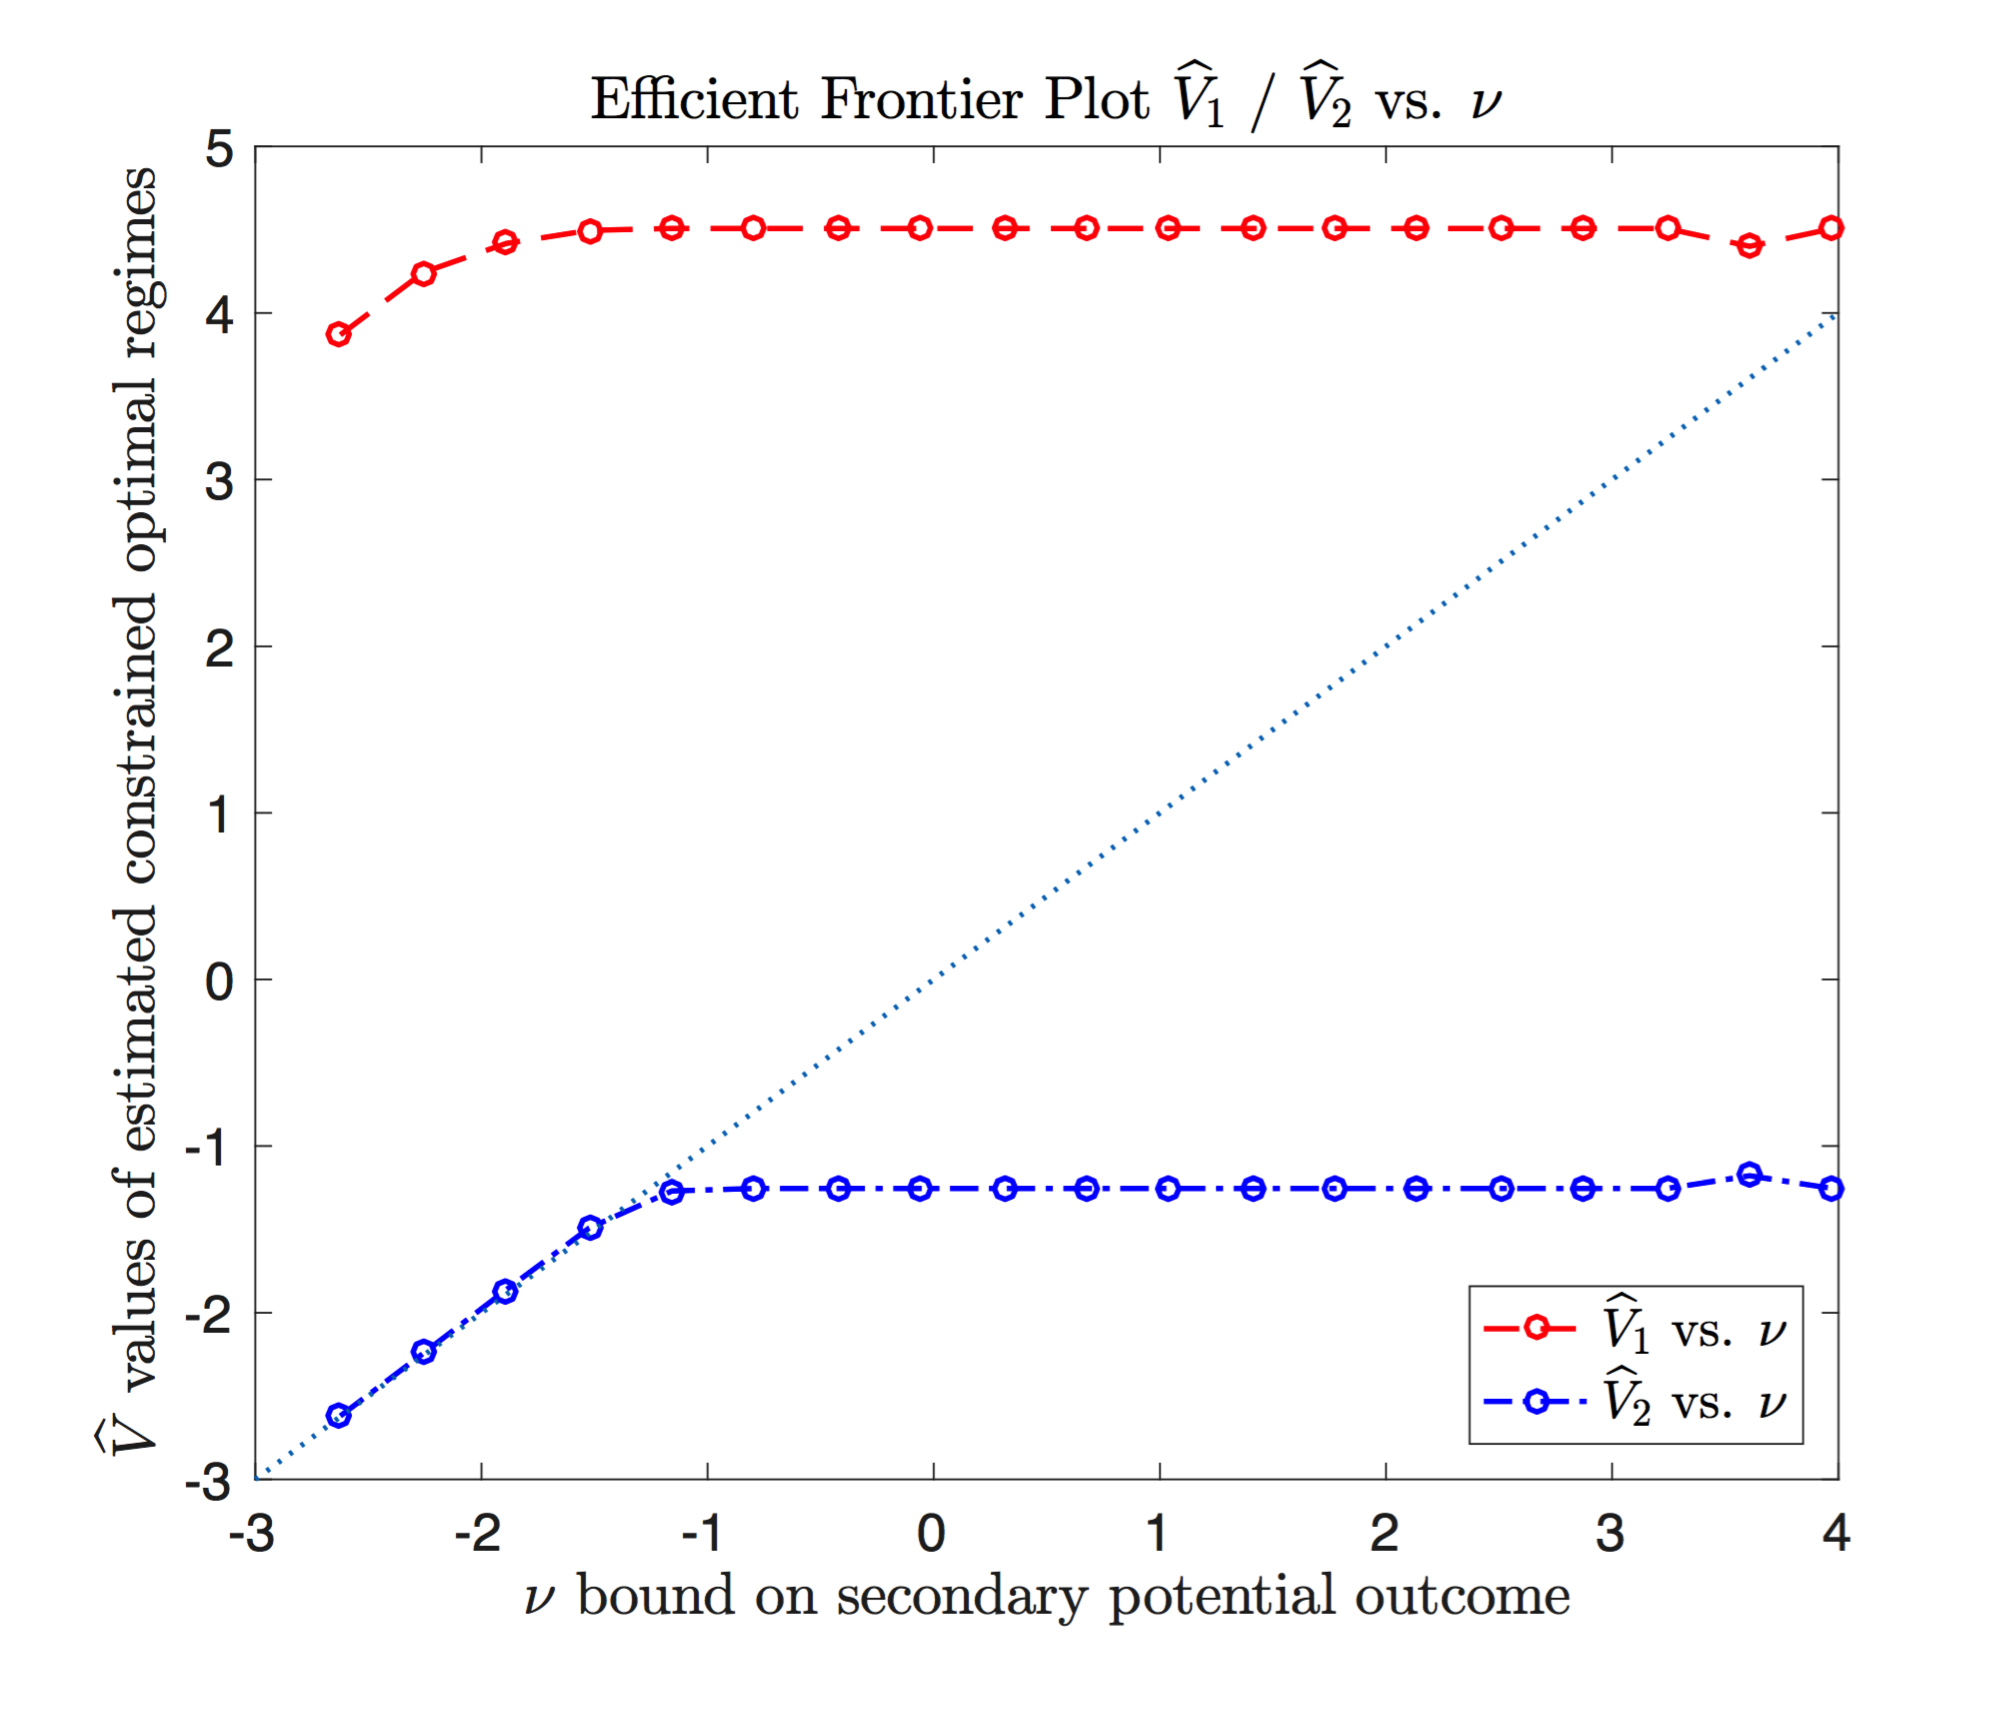
\includegraphics[width=.9\linewidth]{./figs/efficient_plot2.png}
	\caption{Efficient frontier for estimated constrained optimal regimes for Setting 2.}
	\label{fig:2}
	\justify
X-axis is for the values for the constraints $\nu$; Y-axis is for the values of estimated regimes. Red dashed line is for the values in terms of the primary outcome of interest. Blue dashed line is for the values in terms of the secondary outcome of interest.
\end{figure}
\begin{table}[!htbp]
	\caption {Simulation Result for Setting 3}
	\centering
	{\tt
		\begin{tabular}{rrrrrrrrrr}\hline 
$\nu$  & $\wh{V}_1(\wh{\bs{\theta}}_{\nu})$ & $std(\wh{V}_1)$ & $\wh{V}_2(\wh{\bs{\theta}}_{\nu})$ & $std(\wh{V}_2)$ & $\wh{\theta}_{\nu,1}$ & $std(\wh{\theta}_{\nu,1})$ & $\wh{\theta}_{\nu,2}$ & $std(\wh{\theta}_{\nu,2})$ \\ \hline 
-2.50 &     1.19 &     0.19  &    -2.55 &      0.15 &     -0.05 &      0.10 &      0.99 &      0.01 \\ 
-2.15 &     1.33 &     0.05  &    -2.18 &      0.16 &     -0.24 &      0.07 &      0.97 &      0.02 \\ 
-1.80 &     1.42 &     0.04  &    -1.82 &      0.17 &     -0.39 &      0.06 &      0.92 &      0.03 \\ 
-1.45 &     1.50 &     0.04  &    -1.48 &      0.17 &     -0.51 &      0.06 &      0.86 &      0.03 \\ 
-1.09 &     1.56 &     0.03  &    -1.15 &      0.18 &     -0.60 &      0.05 &      0.79 &      0.04 \\ 
-0.74 &     1.61 &     0.02  &    -0.83 &      0.20 &     -0.69 &      0.05 &      0.72 &      0.04 \\ 
-0.39 &     1.62 &     0.02  &    -0.53 &      0.26 &     -0.75 &      0.06 &      0.66 &      0.06 \\ 
-0.04 &     1.63 &     0.01  &    -0.30 &      0.32 &     -0.79 &      0.06 &      0.61 &      0.07 \\ 
 0.32 &     1.63 &     0.01  &    -0.18 &      0.43 &     -0.81 &      0.07 &      0.58 &      0.10 \\ 
 0.67 &     1.63 &     0.01  &    -0.06 &      0.47 &     -0.82 &      0.08 &      0.55 &      0.11 \\ 
 1.02 &     1.63 &     0.01  &    -0.08 &      0.51 &     -0.82 &      0.08 &      0.55 &      0.12 \\ 
 1.37 &     1.63 &     0.01  &    -0.03 &      0.52 &     -0.83 &      0.08 &      0.54 &      0.13 \\ 
 1.73 &     1.62 &     0.02  &    -0.04 &      0.53 &     -0.83 &      0.08 &      0.54 &      0.13 \\ 
 2.08 &     1.63 &     0.01  &    -0.04 &      0.50 &     -0.83 &      0.08 &      0.54 &      0.12 \\ 
 2.43 &     1.63 &     0.01  &    -0.03 &      0.51 &     -0.83 &      0.08 &      0.54 &      0.12 \\ 
 2.78 &     1.63 &     0.01  &    -0.03 &      0.51 &     -0.83 &      0.08 &      0.54 &      0.12 \\ 
 3.13 &     1.63 &     0.01  &    -0.02 &      0.50 &     -0.83 &      0.08 &      0.54 &      0.12 \\ 
 3.49 &     1.62 &     0.13  &     0.01 &      0.57 &     -0.83 &      0.10 &      0.53 &      0.17 \\ 
 3.84 &     1.63 &     0.01  &     0.00 &      0.52 &     -0.83 &      0.08 &      0.53 &      0.13 \\ \hline 
\end{tabular}

	}
	\justify
	Here, $\nu$ denotes the values of the constraint; $\wh{V}_1(\wh{\bs{\theta}}_{\nu})$ denotes the values of estimated regimes in terms of primary outcome of interest; $std(\wh{V}_1)$ denotes the standard deviation of the estimated regime values in terms of primary outcome of interest; $\wh{V}_2(\wh{\bs{\theta}}_{\nu})$ denotes the values of estimated regimes in terms of secondary outcome of interest; $std(\wh{V}_2)$ denotes the standard deviation of the estimated regime values in terms of secondary outcome of interest; $\wh{\theta}_{\nu,1}$ and $\wh{\theta}_{\nu,2}$ denote the estimated index parameters of the regimes; $std(\wh{\theta}_{\nu,1})$ and $std(\wh{\theta}_{\nu,2})$ denote the standard deviations of those estimated index parameters.	
\end{table} 
\begin{figure}[!htb]
	\centering
	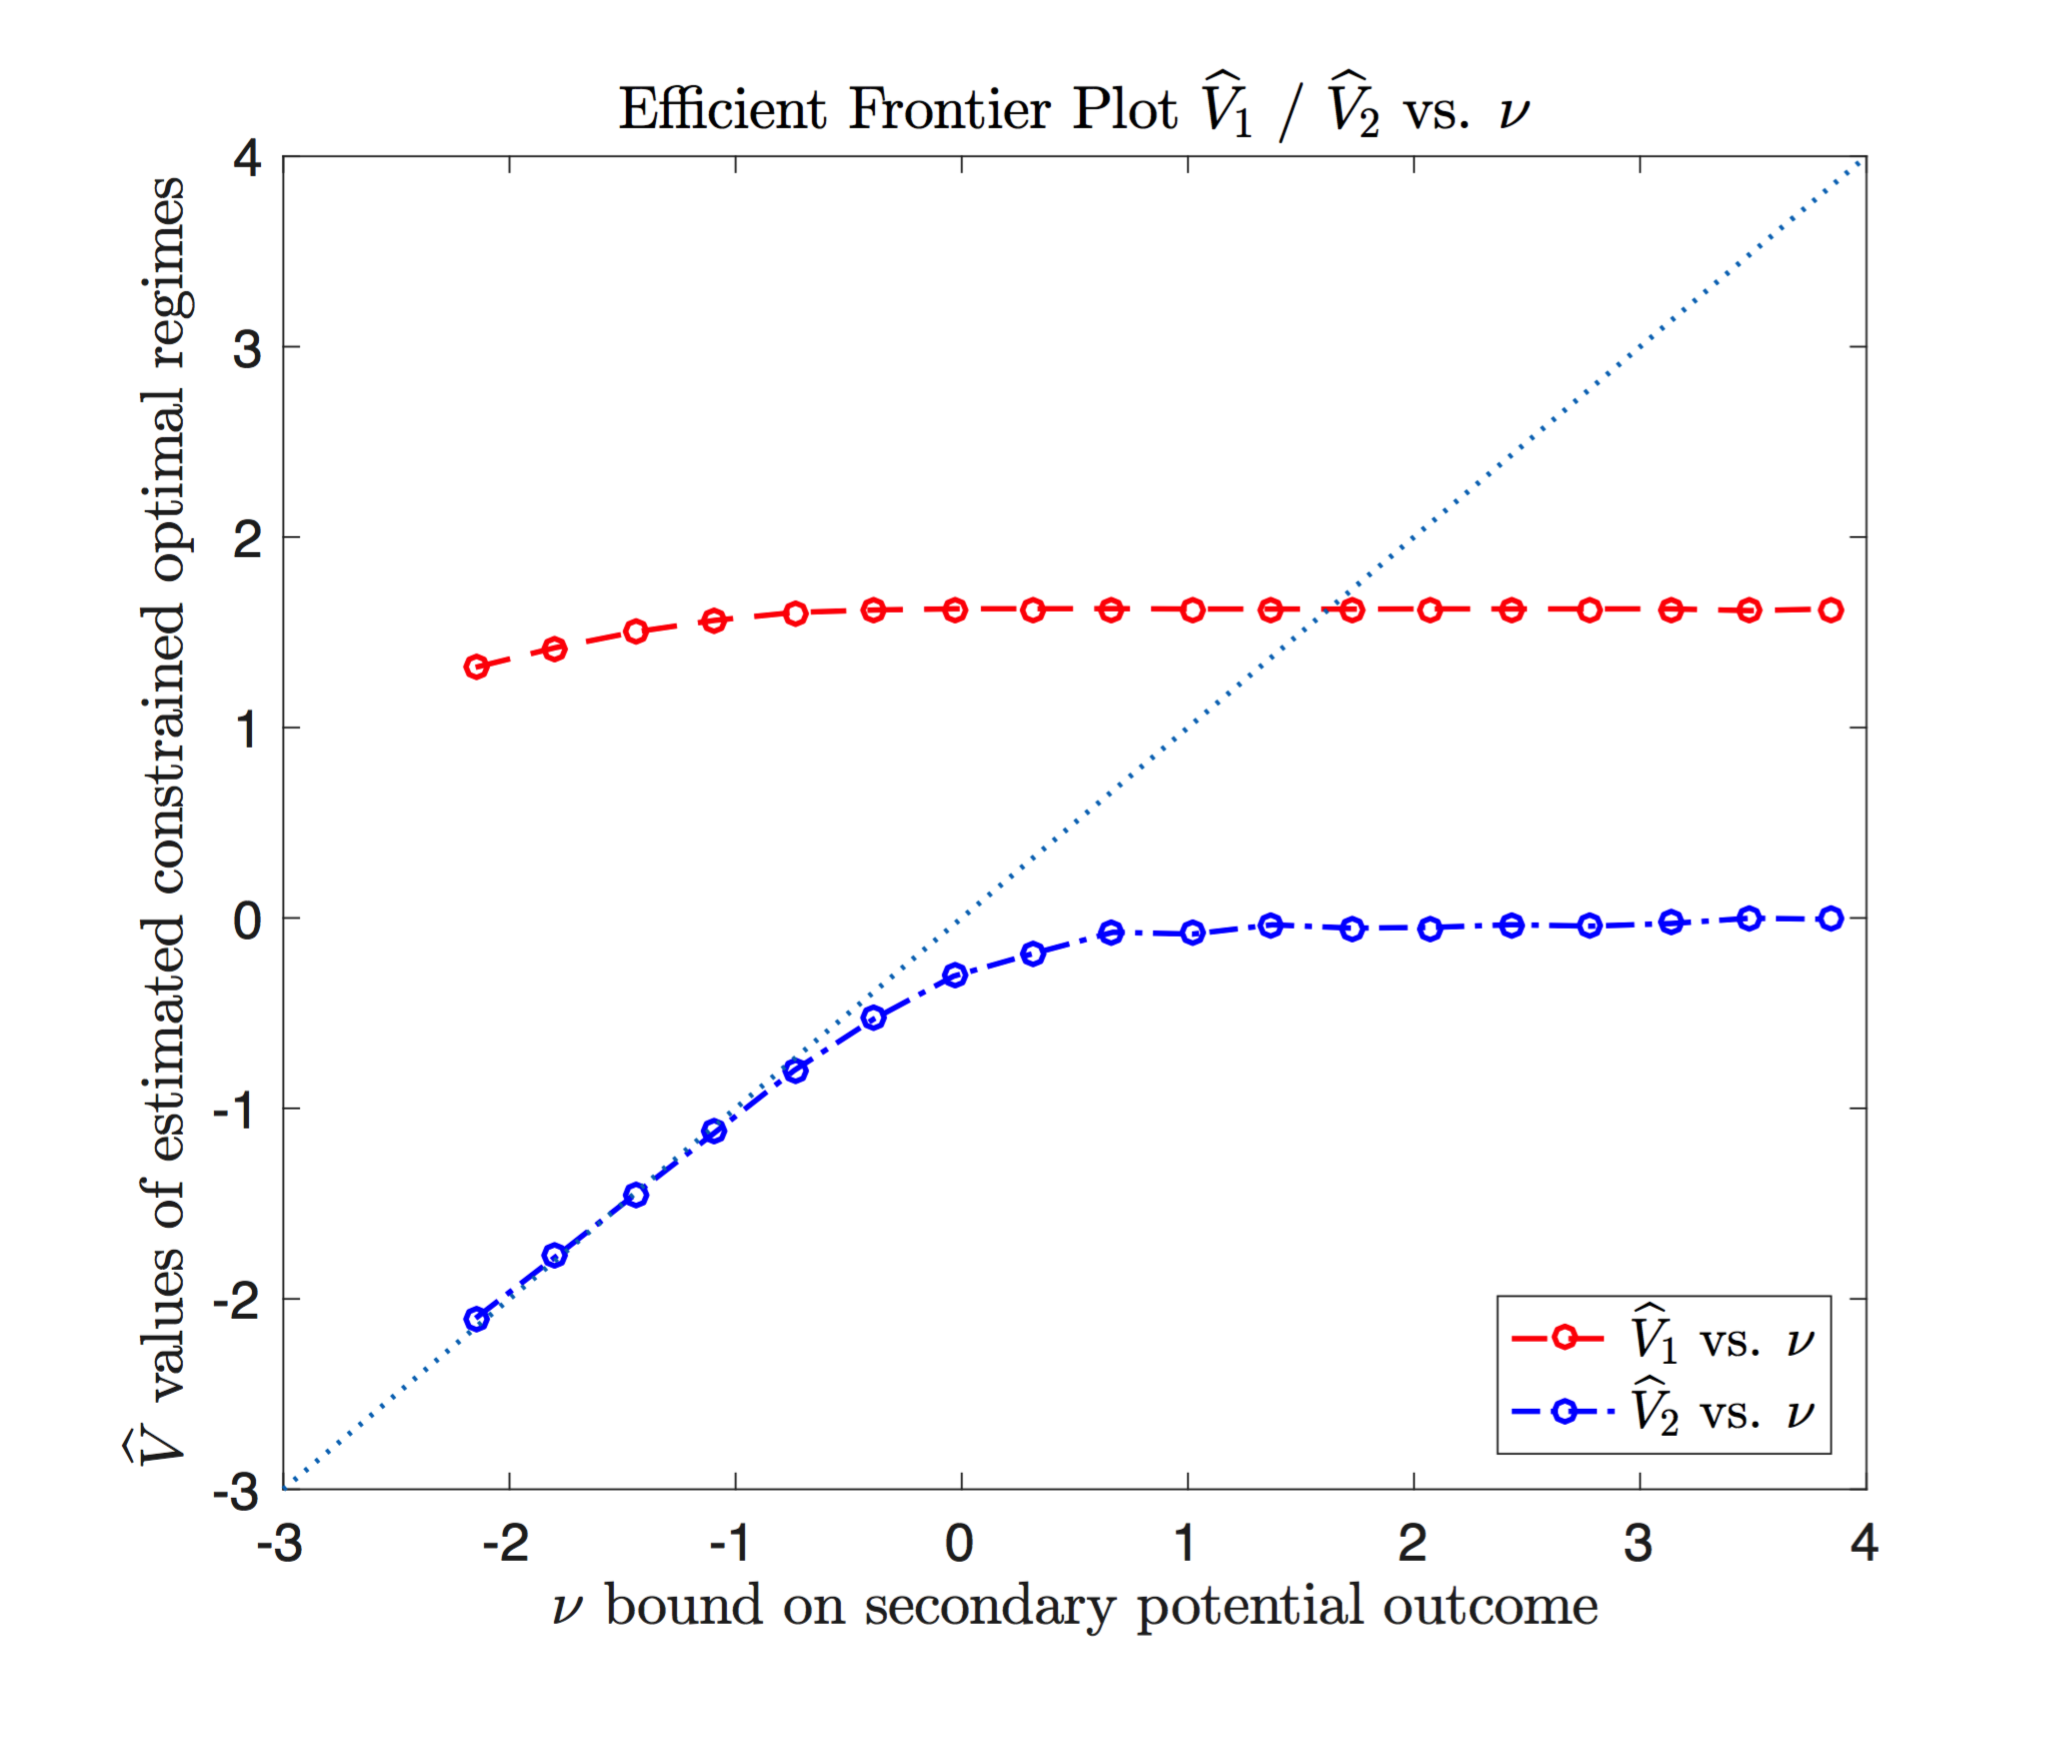
\includegraphics[width=.9\linewidth]{./figs/efficient_plot3.png}
	\caption{Efficient frontier for estimated constrained optimal regimes for Setting 3.}
	\label{fig:3}
	\justify
X-axis is for the values for the constraints $\nu$; Y-axis is for the values of estimated regimes. Red dashed line is for the values in terms of the primary outcome of interest. Blue dashed line is for the values in terms of the secondary outcome of interest.
\end{figure}
\begin{table}[!htbp]
	\caption {Simulation Result for Setting 4}
	\centering
	{\tt
		\begin{tabular}{rrrrrrrrrr}\hline 
$\nu$  & $\wh{V}_1(\wh{\bs{\theta}}_{\nu})$ & $std(\wh{V}_1)$ & $\wh{V}_2(\wh{\bs{\theta}}_{\nu})$ & $std(\wh{V}_2)$ & $\wh{\theta}_{\nu,1}$ & $std(\wh{\theta}_{\nu,1})$ & $\wh{\theta}_{\nu,2}$ & $std(\wh{\theta}_{\nu,2})$ \\ \hline 
%4 &      NaN &      NaN &      NaN  &      NaN &       NaN &       NaN &       NaN &       NaN &       NaN \\ 
%4 &      NaN &      NaN &      NaN  &      NaN &       NaN &       NaN &       NaN &       NaN &       NaN \\ 
%4 &    -1.81 &      NaN &      NaN  &      NaN &       NaN &       NaN &       NaN &       NaN &       NaN \\ 
-1.57 &     1.62 &     0.01  &    -1.82 &      0.03 &      0.14 &      0.12 &     -0.98 &      0.02 \\ 
-1.32 &     1.62 &     0.02  &    -1.81 &      0.04 &      0.14 &      0.13 &     -0.98 &      0.02 \\ 
-1.08 &     1.62 &     0.02  &    -1.82 &      0.03 &      0.15 &      0.13 &     -0.98 &      0.02 \\ 
-0.84 &     1.62 &     0.02  &    -1.81 &      0.04 &      0.14 &      0.13 &     -0.98 &      0.02 \\ 
-0.59 &     1.62 &     0.02  &    -1.81 &      0.04 &      0.14 &      0.13 &     -0.98 &      0.02 \\ 
-0.35 &     1.62 &     0.02  &    -1.81 &      0.04 &      0.14 &      0.13 &     -0.98 &      0.02 \\ 
-0.10 &     1.62 &     0.02  &    -1.81 &      0.04 &      0.14 &      0.13 &     -0.98 &      0.02 \\ 
 0.14 &     1.62 &     0.02  &    -1.81 &      0.04 &      0.14 &      0.13 &     -0.98 &      0.02 \\ 
 0.38 &     1.62 &     0.02  &    -1.81 &      0.04 &      0.14 &      0.13 &     -0.98 &      0.02 \\ 
 0.63 &     1.62 &     0.02  &    -1.81 &      0.04 &      0.14 &      0.13 &     -0.98 &      0.02 \\ 
 0.87 &     1.62 &     0.02  &    -1.81 &      0.04 &      0.14 &      0.14 &     -0.98 &      0.02 \\ 
 1.11 &     1.62 &     0.02  &    -1.81 &      0.04 &      0.14 &      0.13 &     -0.98 &      0.02 \\ 
 1.36 &     1.62 &     0.02  &    -1.81 &      0.04 &      0.15 &      0.13 &     -0.98 &      0.02 \\ 
 1.60 &     1.62 &     0.02  &    -1.81 &      0.04 &      0.14 &      0.13 &     -0.98 &      0.02 \\ 
 1.84 &     1.62 &     0.02  &    -1.81 &      0.04 &      0.14 &      0.13 &     -0.98 &      0.02 \\ 
 2.09 &     1.62 &     0.02  &    -1.81 &      0.04 &      0.14 &      0.13 &     -0.98 &      0.02 \\ 
 2.33 &     1.62 &     0.02  &    -1.81 &      0.04 &      0.14 &      0.13 &     -0.98 &      0.02 \\ 
 2.57 &     1.62 &     0.02  &    -1.81 &      0.04 &      0.14 &      0.13 &     -0.98 &      0.02 \\ 
 2.82 &     1.62 &     0.02  &    -1.81 &      0.04 &      0.14 &      0.13 &     -0.98 &      0.02 \\ \hline 
\end{tabular}

	}
	\justify
	Here, $\nu$ denotes the values of the constraint; $\wh{V}_1(\wh{\bs{\theta}}_{\nu})$ denotes the values of estimated regimes in terms of primary outcome of interest; $std(\wh{V}_1)$ denotes the standard deviation of the estimated regime values in terms of primary outcome of interest; $\wh{V}_2(\wh{\bs{\theta}}_{\nu})$ denotes the values of estimated regimes in terms of secondary outcome of interest; $std(\wh{V}_2)$ denotes the standard deviation of the estimated regime values in terms of secondary outcome of interest; $\wh{\theta}_{\nu,1}$ and $\wh{\theta}_{\nu,2}$ denote the estimated index parameters of the regimes; $std(\wh{\theta}_{\nu,1})$ and $std(\wh{\theta}_{\nu,2})$ denote the standard deviations of those estimated index parameters.	
\end{table} 
\begin{figure}[!htb]
	\centering
	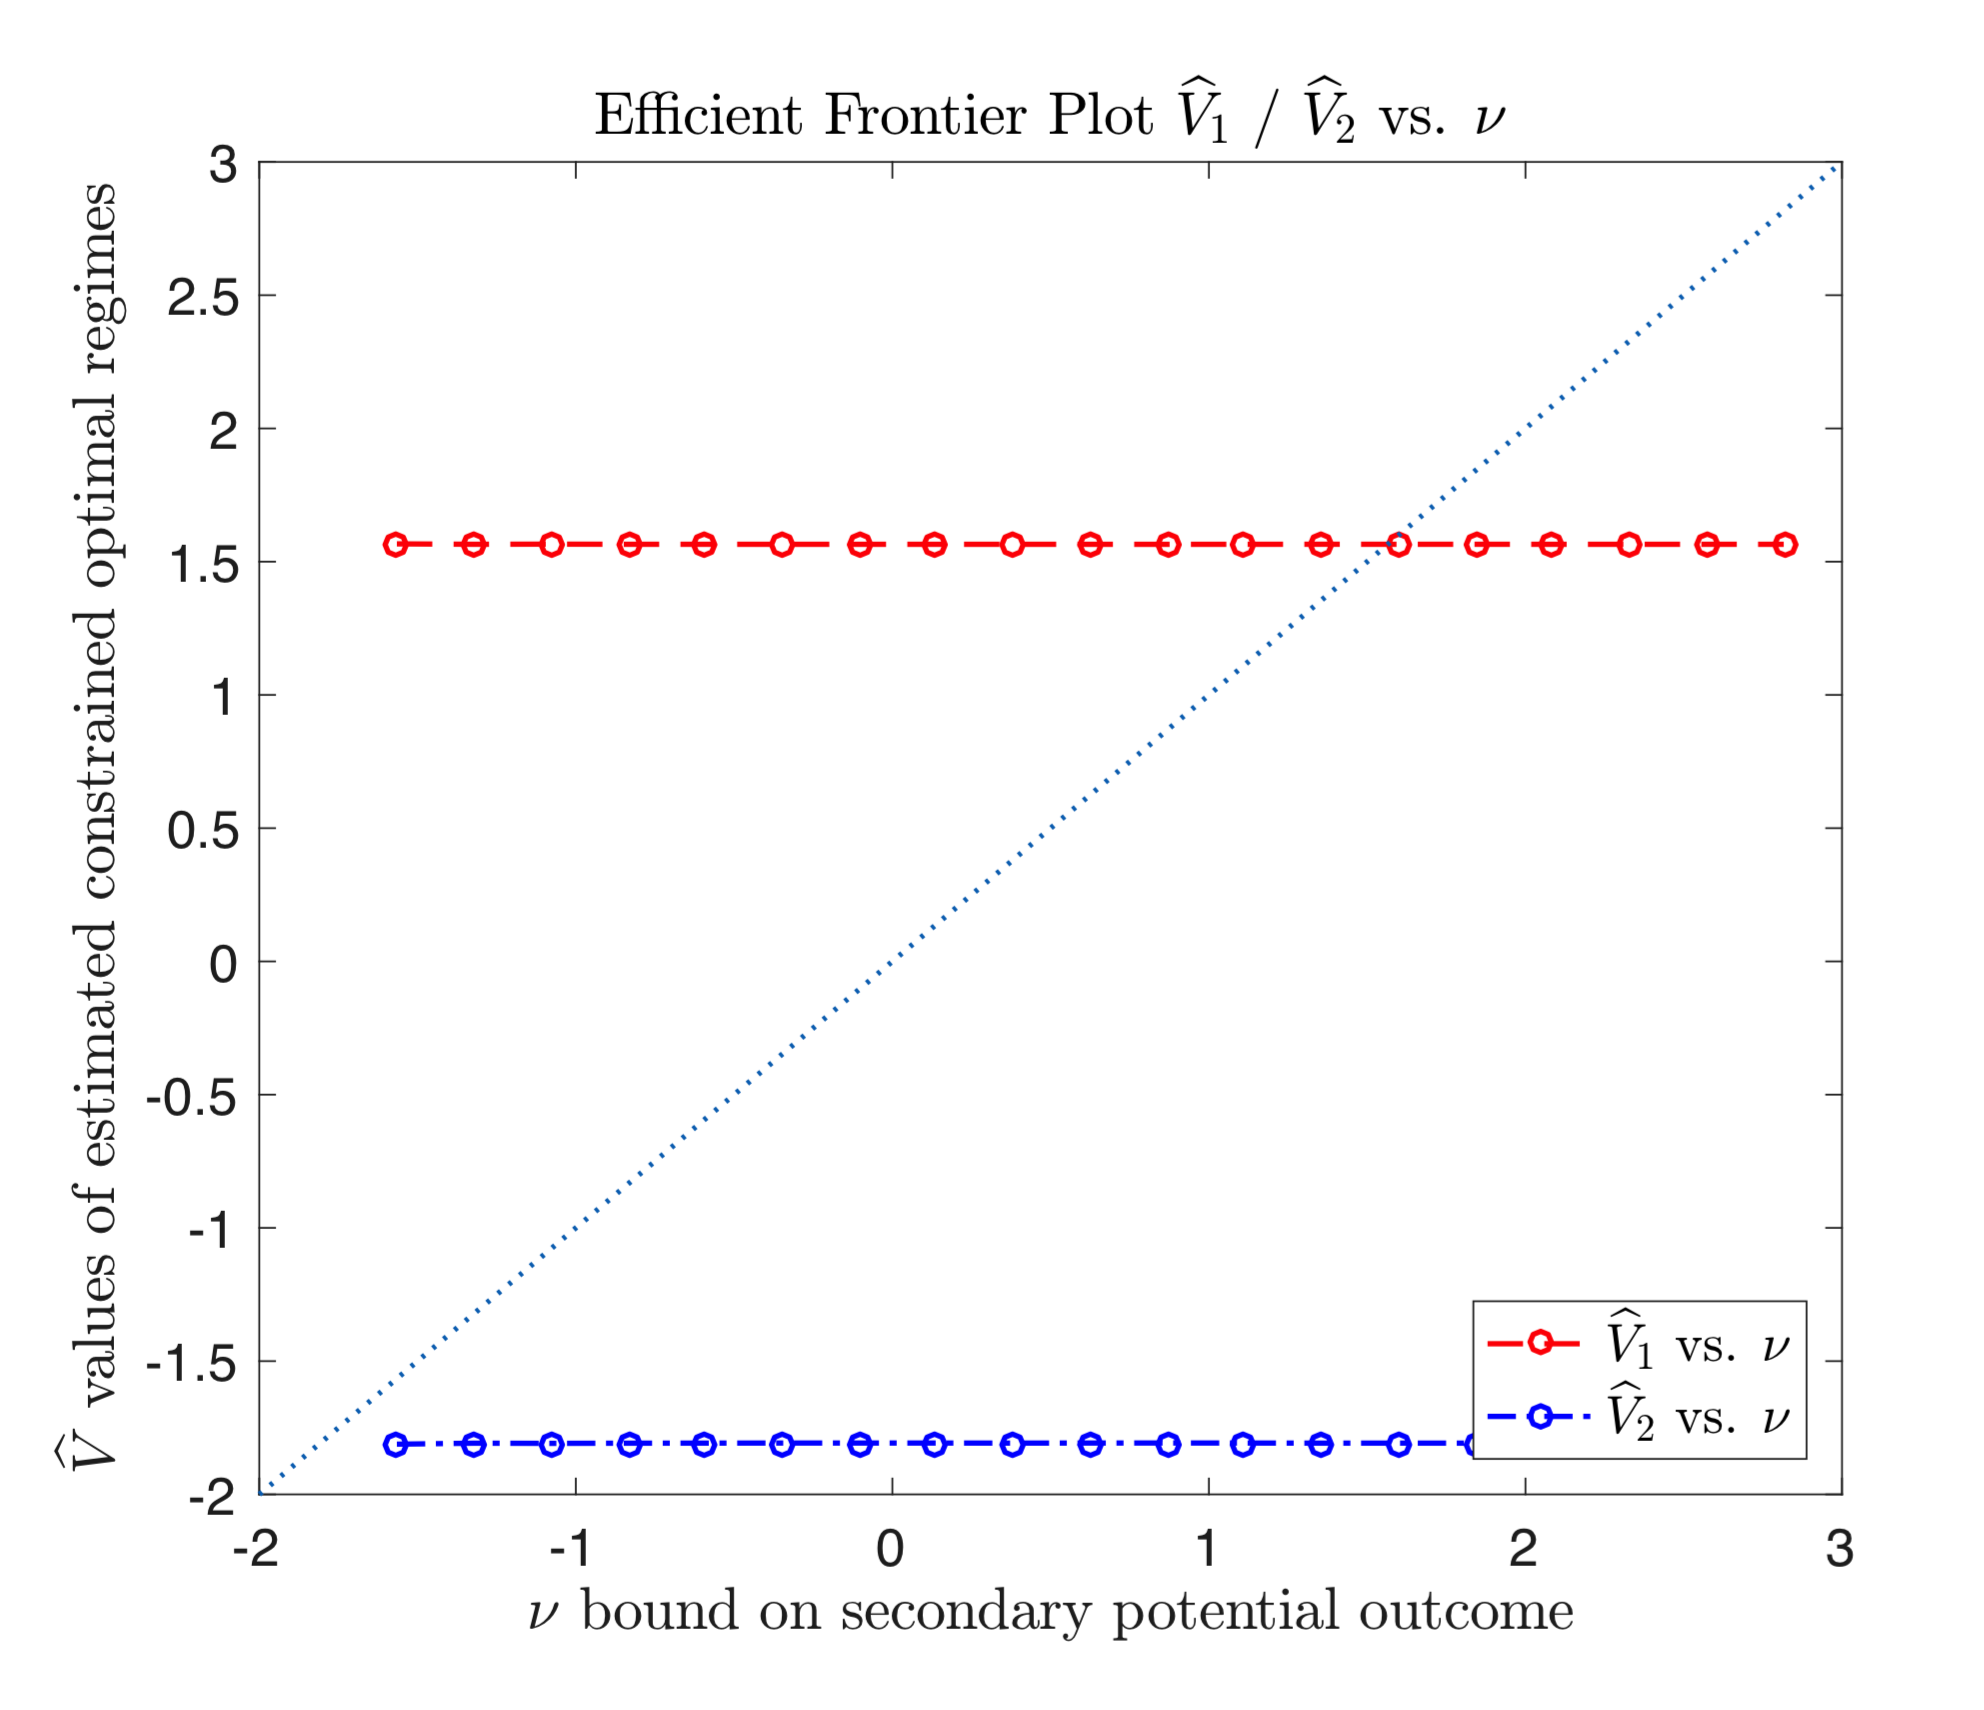
\includegraphics[width=.9\linewidth]{./figs/efficient_plot4.png}
	\caption{Efficient frontier for estimated constrained optimal regimes for Setting 4.}
	\label{fig:4}
	\justify
X-axis is for the values for the constraints $\nu$; Y-axis is for the values of estimated regimes. Red dashed line is for the values in terms of the primary outcome of interest. Blue dashed line is for the values in terms of the secondary outcome of interest.
\end{figure}
\begin{table}[!htbp]
	\caption {Simulation Result for Setting 5}
	\centering
	{\tt
		\begin{tabular}{rrrrrrrrrr}\hline 
setting & $\nu$  & $\wh{V}_1(\wh{\bs{\theta}}_{\nu})$ & $std(\wh{V}_1)$ & $\wh{V}_2(\wh{\bs{\theta}}_{\nu})$ & $std(\wh{V}_2)$ & $\wh{\theta}_{\nu,1}$ & $std(\wh{\theta}_{\nu,1})$ & $\wh{\theta}_{\nu,2}$ & $std(\wh{\theta}_{\nu,2})$ \\ \hline 
5 &    -2.22 &     0.63 &     0.03  &    -2.30 &      0.21 &      0.90 &      0.07 &     -0.42 &      0.11 \\ 
5 &    -1.85 &     0.67 &     0.03  &    -1.97 &      0.25 &      0.95 &      0.07 &     -0.27 &      0.12 \\ 
5 &    -1.49 &     0.69 &     0.03  &    -1.67 &      0.34 &      0.98 &      0.05 &     -0.16 &      0.14 \\ 
5 &    -1.13 &     0.71 &     0.04  &    -1.36 &      0.40 &      0.99 &      0.04 &     -0.05 &      0.15 \\ 
5 &    -0.77 &     0.73 &     0.04  &    -1.10 &      0.47 &      0.98 &      0.03 &      0.04 &      0.17 \\ 
5 &    -0.40 &     0.74 &     0.05  &    -0.88 &      0.61 &      0.97 &      0.06 &      0.10 &      0.22 \\ 
5 &    -0.04 &     0.75 &     0.06  &    -0.61 &      0.66 &      0.95 &      0.13 &      0.18 &      0.22 \\ 
5 &     0.32 &     0.75 &     0.07  &    -0.38 &      0.78 &      0.92 &      0.15 &      0.24 &      0.27 \\ 
5 &     0.68 &     0.76 &     0.06  &    -0.18 &      0.84 &      0.91 &      0.15 &      0.29 &      0.26 \\ 
5 &     1.05 &     0.76 &     0.07  &    -0.03 &      0.94 &      0.88 &      0.19 &      0.33 &      0.28 \\ 
5 &     1.41 &     0.77 &     0.07  &     0.15 &      0.98 &      0.86 &      0.20 &      0.37 &      0.28 \\ 
5 &     1.77 &     0.77 &     0.05  &     0.19 &      1.04 &      0.86 &      0.17 &      0.39 &      0.29 \\ 
5 &     2.13 &     0.77 &     0.05  &     0.29 &      1.10 &      0.84 &      0.18 &      0.41 &      0.30 \\ 
5 &     2.50 &     0.77 &     0.05  &     0.33 &      1.13 &      0.83 &      0.19 &      0.42 &      0.31 \\ 
5 &     2.86 &     0.77 &     0.04  &     0.42 &      1.19 &      0.82 &      0.17 &      0.44 &      0.31 \\ 
5 &     3.22 &     0.77 &     0.03  &     0.48 &      1.20 &      0.81 &      0.19 &      0.46 &      0.31 \\ 
5 &     3.58 &     0.77 &     0.03  &     0.39 &      1.19 &      0.83 &      0.18 &      0.44 &      0.31 \\ 
5 &     3.94 &     0.77 &     0.04  &     0.52 &      1.28 &      0.80 &      0.22 &      0.46 &      0.32 \\ \hline 
\end{tabular}

	}
	\justify
	Here, $\nu$ denotes the values of the constraint; $\wh{V}_1(\wh{\bs{\theta}}_{\nu})$ denotes the values of estimated regimes in terms of primary outcome of interest; $std(\wh{V}_1)$ denotes the standard deviation of the estimated regime values in terms of primary outcome of interest; $\wh{V}_2(\wh{\bs{\theta}}_{\nu})$ denotes the values of estimated regimes in terms of secondary outcome of interest; $std(\wh{V}_2)$ denotes the standard deviation of the estimated regime values in terms of secondary outcome of interest; $\wh{\theta}_{\nu,1}$ and $\wh{\theta}_{\nu,2}$ denote the estimated index parameters of the regimes; $std(\wh{\theta}_{\nu,1})$ and $std(\wh{\theta}_{\nu,2})$ denote the standard deviations of those estimated index parameters.	
\end{table} 
\begin{figure}[!htb]
	\centering
	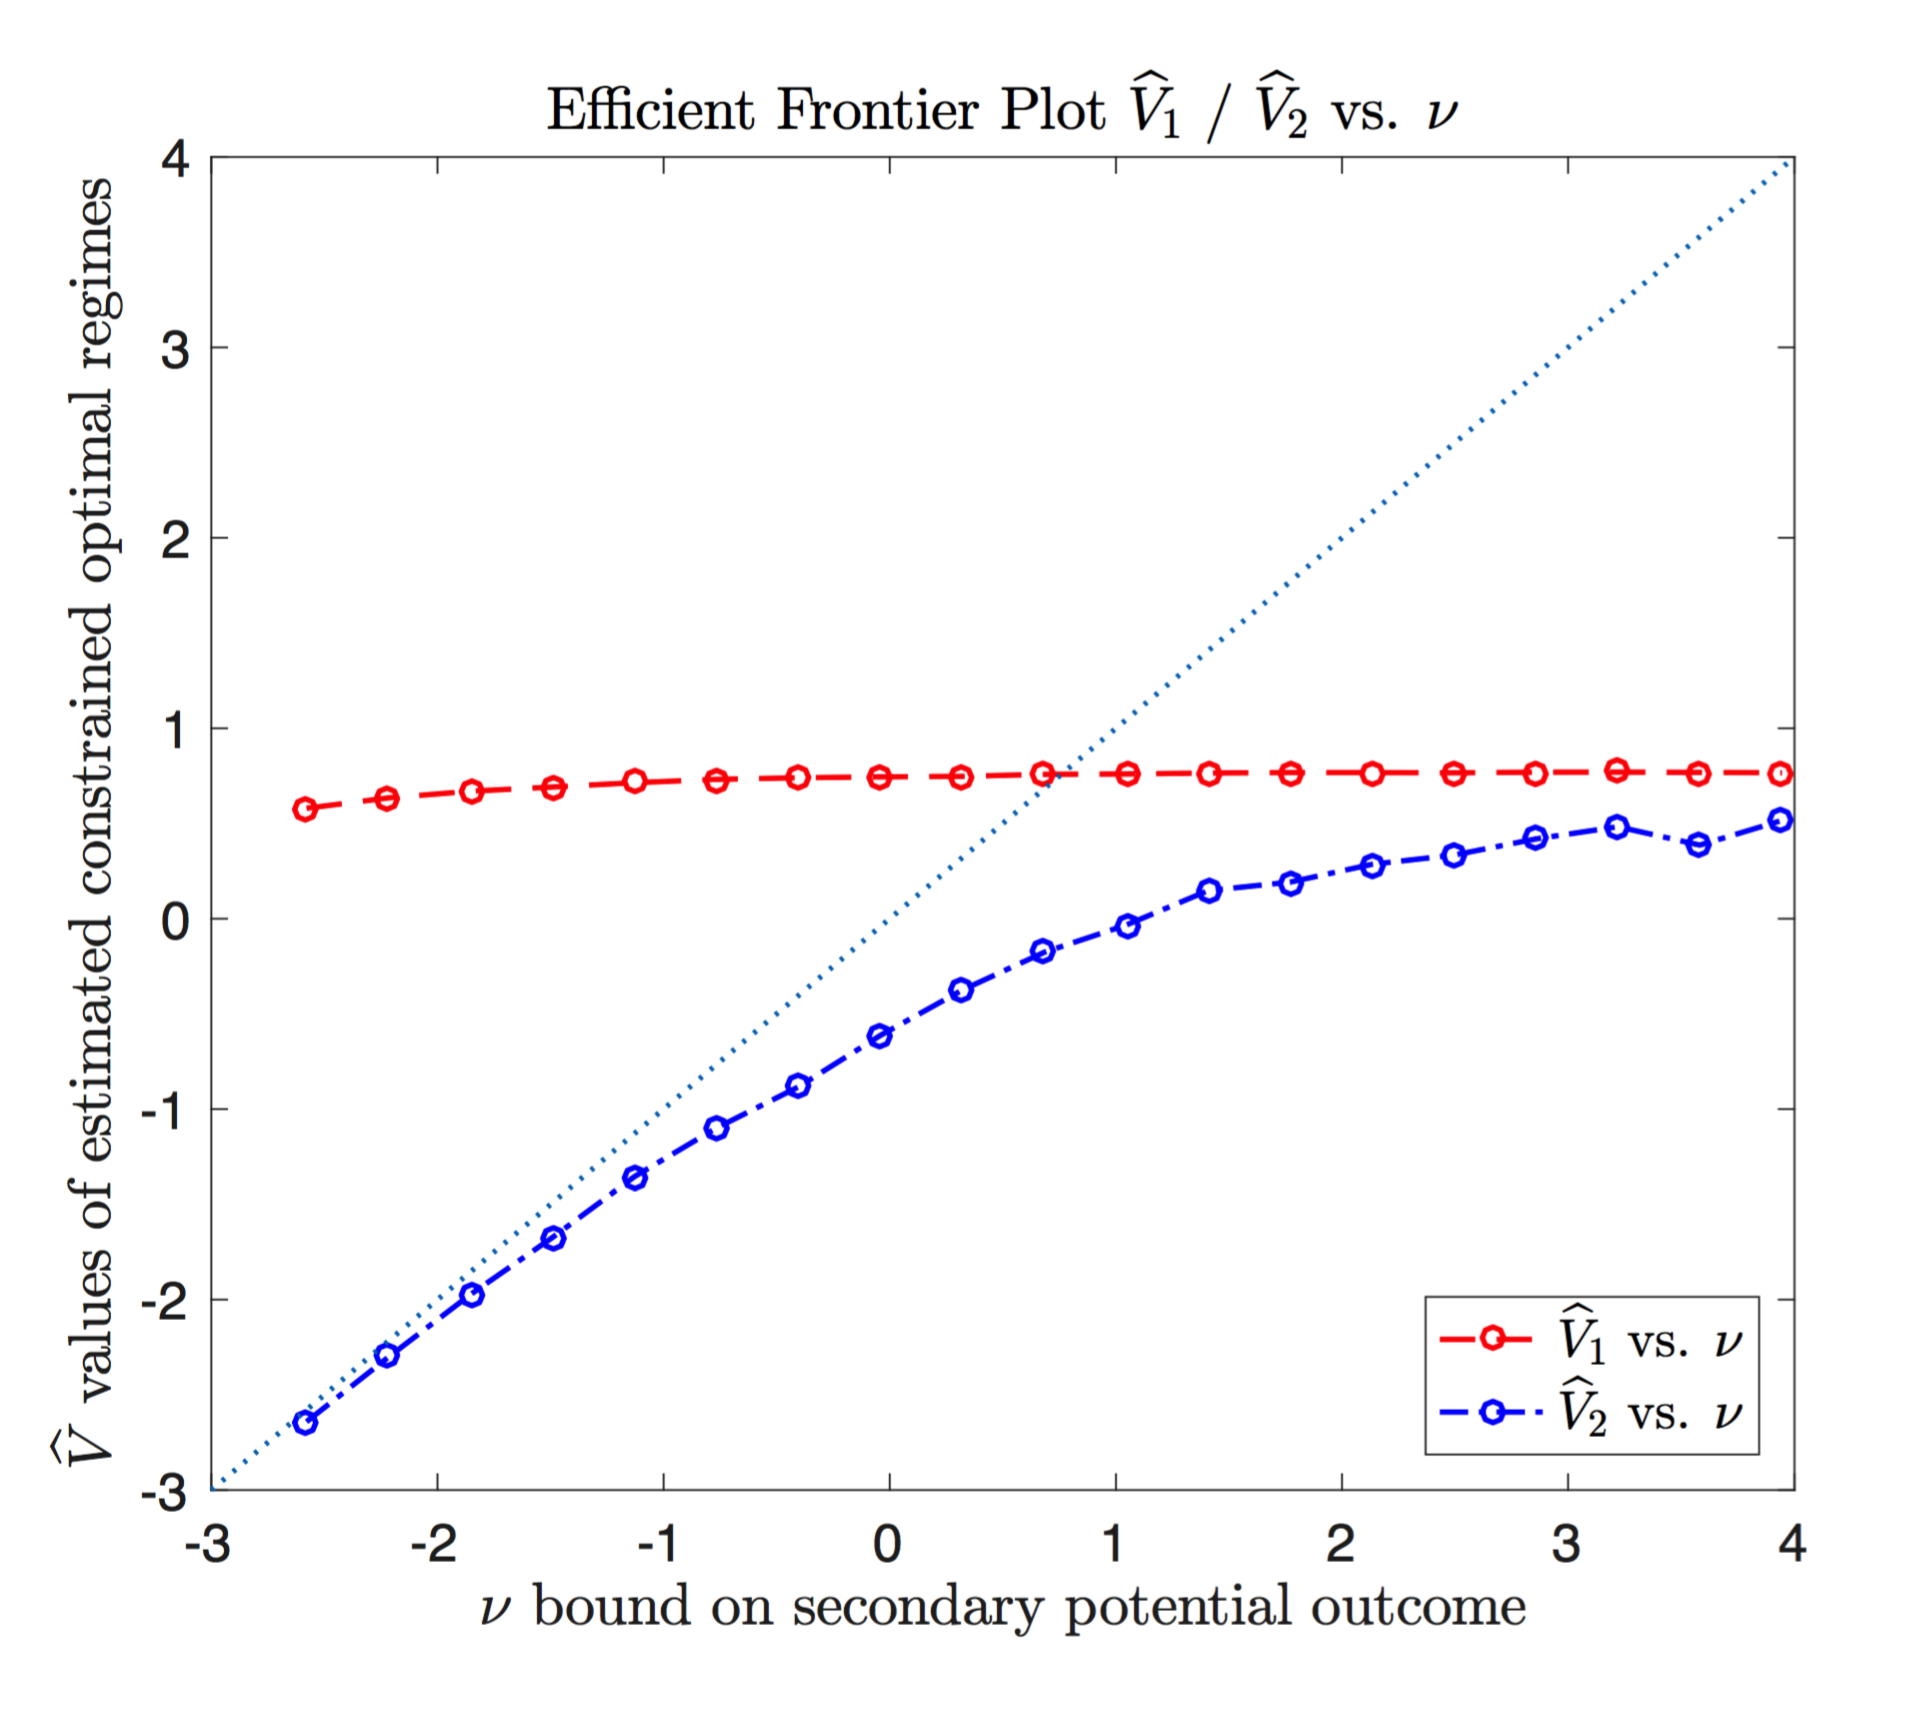
\includegraphics[width=.9\linewidth]{./figs/efficient_plot5.png}
	\caption{Efficient frontier for estimated constrained optimal regimes for Setting 5.}
	\label{fig:5}
	\justify
X-axis is for the values for the constraints $\nu$; Y-axis is for the values of estimated regimes. Red dashed line is for the values in terms of the primary outcome of interest. Blue dashed line is for the values in terms of the secondary outcome of interest.
\end{figure}
\begin{table}[!htbp]
	\caption {Simulation Result for Setting 6}
	\centering
	{\tt
		\begin{tabular}{rrrrrrrrrr}\hline 
$\nu$  & $\wh{V}_1(\wh{\bs{\theta}}_{\nu})$ & $std(\wh{V}_1)$ & $\wh{V}_2(\wh{\bs{\theta}}_{\nu})$ & $std(\wh{V}_2)$ & $\wh{\theta}_{\nu,1}$ & $std(\wh{\theta}_{\nu,1})$ & $\wh{\theta}_{\nu,2}$ & $std(\wh{\theta}_{\nu,2})$ \\ \hline 
%6 &      NaN &      NaN &      NaN  &      NaN &       NaN &       NaN &       NaN &       NaN &       NaN \\ 
%6 &      NaN &      NaN &      NaN  &      NaN &       NaN &       NaN &       NaN &       NaN &       NaN \\ 
%6 &    -0.61 &      NaN &      NaN  &      NaN &       NaN &       NaN &       NaN &       NaN &       NaN \\ 
-0.50 &     0.59 &     0.11  &    -0.55 &      0.41 &     -0.83 &      0.31 &     -0.44 &      0.13 \\ 
-0.38 &     0.73 &     0.08  &    -0.36 &      0.07 &     -0.96 &      0.03 &     -0.26 &      0.11 \\ 
-0.26 &     0.85 &     0.07  &    -0.25 &      0.08 &     -0.99 &      0.01 &     -0.11 &      0.10 \\ 
-0.14 &     0.94 &     0.06  &    -0.13 &      0.09 &     -1.00 &      0.01 &      0.02 &      0.09 \\ 
-0.03 &     1.01 &     0.05  &    -0.00 &      0.09 &     -0.99 &      0.01 &      0.15 &      0.08 \\ 
 0.09 &     1.07 &     0.04  &     0.12 &      0.09 &     -0.96 &      0.02 &      0.26 &      0.08 \\ 
 0.21 &     1.12 &     0.03  &     0.24 &      0.09 &     -0.93 &      0.03 &      0.36 &      0.07 \\ 
 0.33 &     1.15 &     0.14  &     0.36 &      0.09 &     -0.87 &      0.17 &      0.45 &      0.13 \\ 
 0.44 &     1.18 &     0.14  &     0.48 &      0.08 &     -0.82 &      0.17 &      0.54 &      0.13 \\ 
 0.56 &     1.21 &     0.14  &     0.60 &      0.09 &     -0.76 &      0.17 &      0.62 &      0.13 \\ 
 0.68 &     1.20 &     0.25  &     0.71 &      0.09 &     -0.65 &      0.30 &      0.67 &      0.22 \\ 
 0.80 &     1.23 &     0.19  &     0.80 &      0.09 &     -0.61 &      0.23 &      0.74 &      0.17 \\ 
 0.91 &     1.23 &     0.18  &     0.88 &      0.10 &     -0.56 &      0.23 &      0.78 &      0.16 \\ 
 1.03 &     1.25 &     0.09  &     0.92 &      0.12 &     -0.54 &      0.15 &      0.82 &      0.10 \\ 
 1.15 &     1.26 &     0.01  &     0.95 &      0.14 &     -0.52 &      0.12 &      0.84 &      0.08 \\ 
 1.27 &     1.25 &     0.01  &     0.96 &      0.15 &     -0.51 &      0.13 &      0.85 &      0.08 \\ 
 1.38 &     1.25 &     0.01  &     0.96 &      0.15 &     -0.51 &      0.12 &      0.85 &      0.08 \\ 
 1.50 &     1.25 &     0.01  &     0.96 &      0.15 &     -0.51 &      0.13 &      0.85 &      0.08 \\ 
 1.62 &     1.25 &     0.01  &     0.96 &      0.15 &     -0.51 &      0.13 &      0.85 &      0.08 \\ \hline 
\end{tabular}

	}
	\justify
	Here, $\nu$ denotes the values of the constraint; $\wh{V}_1(\wh{\bs{\theta}}_{\nu})$ denotes the values of estimated regimes in terms of primary outcome of interest; $std(\wh{V}_1)$ denotes the standard deviation of the estimated regime values in terms of primary outcome of interest; $\wh{V}_2(\wh{\bs{\theta}}_{\nu})$ denotes the values of estimated regimes in terms of secondary outcome of interest; $std(\wh{V}_2)$ denotes the standard deviation of the estimated regime values in terms of secondary outcome of interest; $\wh{\theta}_{\nu,1}$ and $\wh{\theta}_{\nu,2}$ denote the estimated index parameters of the regimes; $std(\wh{\theta}_{\nu,1})$ and $std(\wh{\theta}_{\nu,2})$ denote the standard deviations of those estimated index parameters.	
\end{table} 
\begin{figure}[!htb]
	\centering
	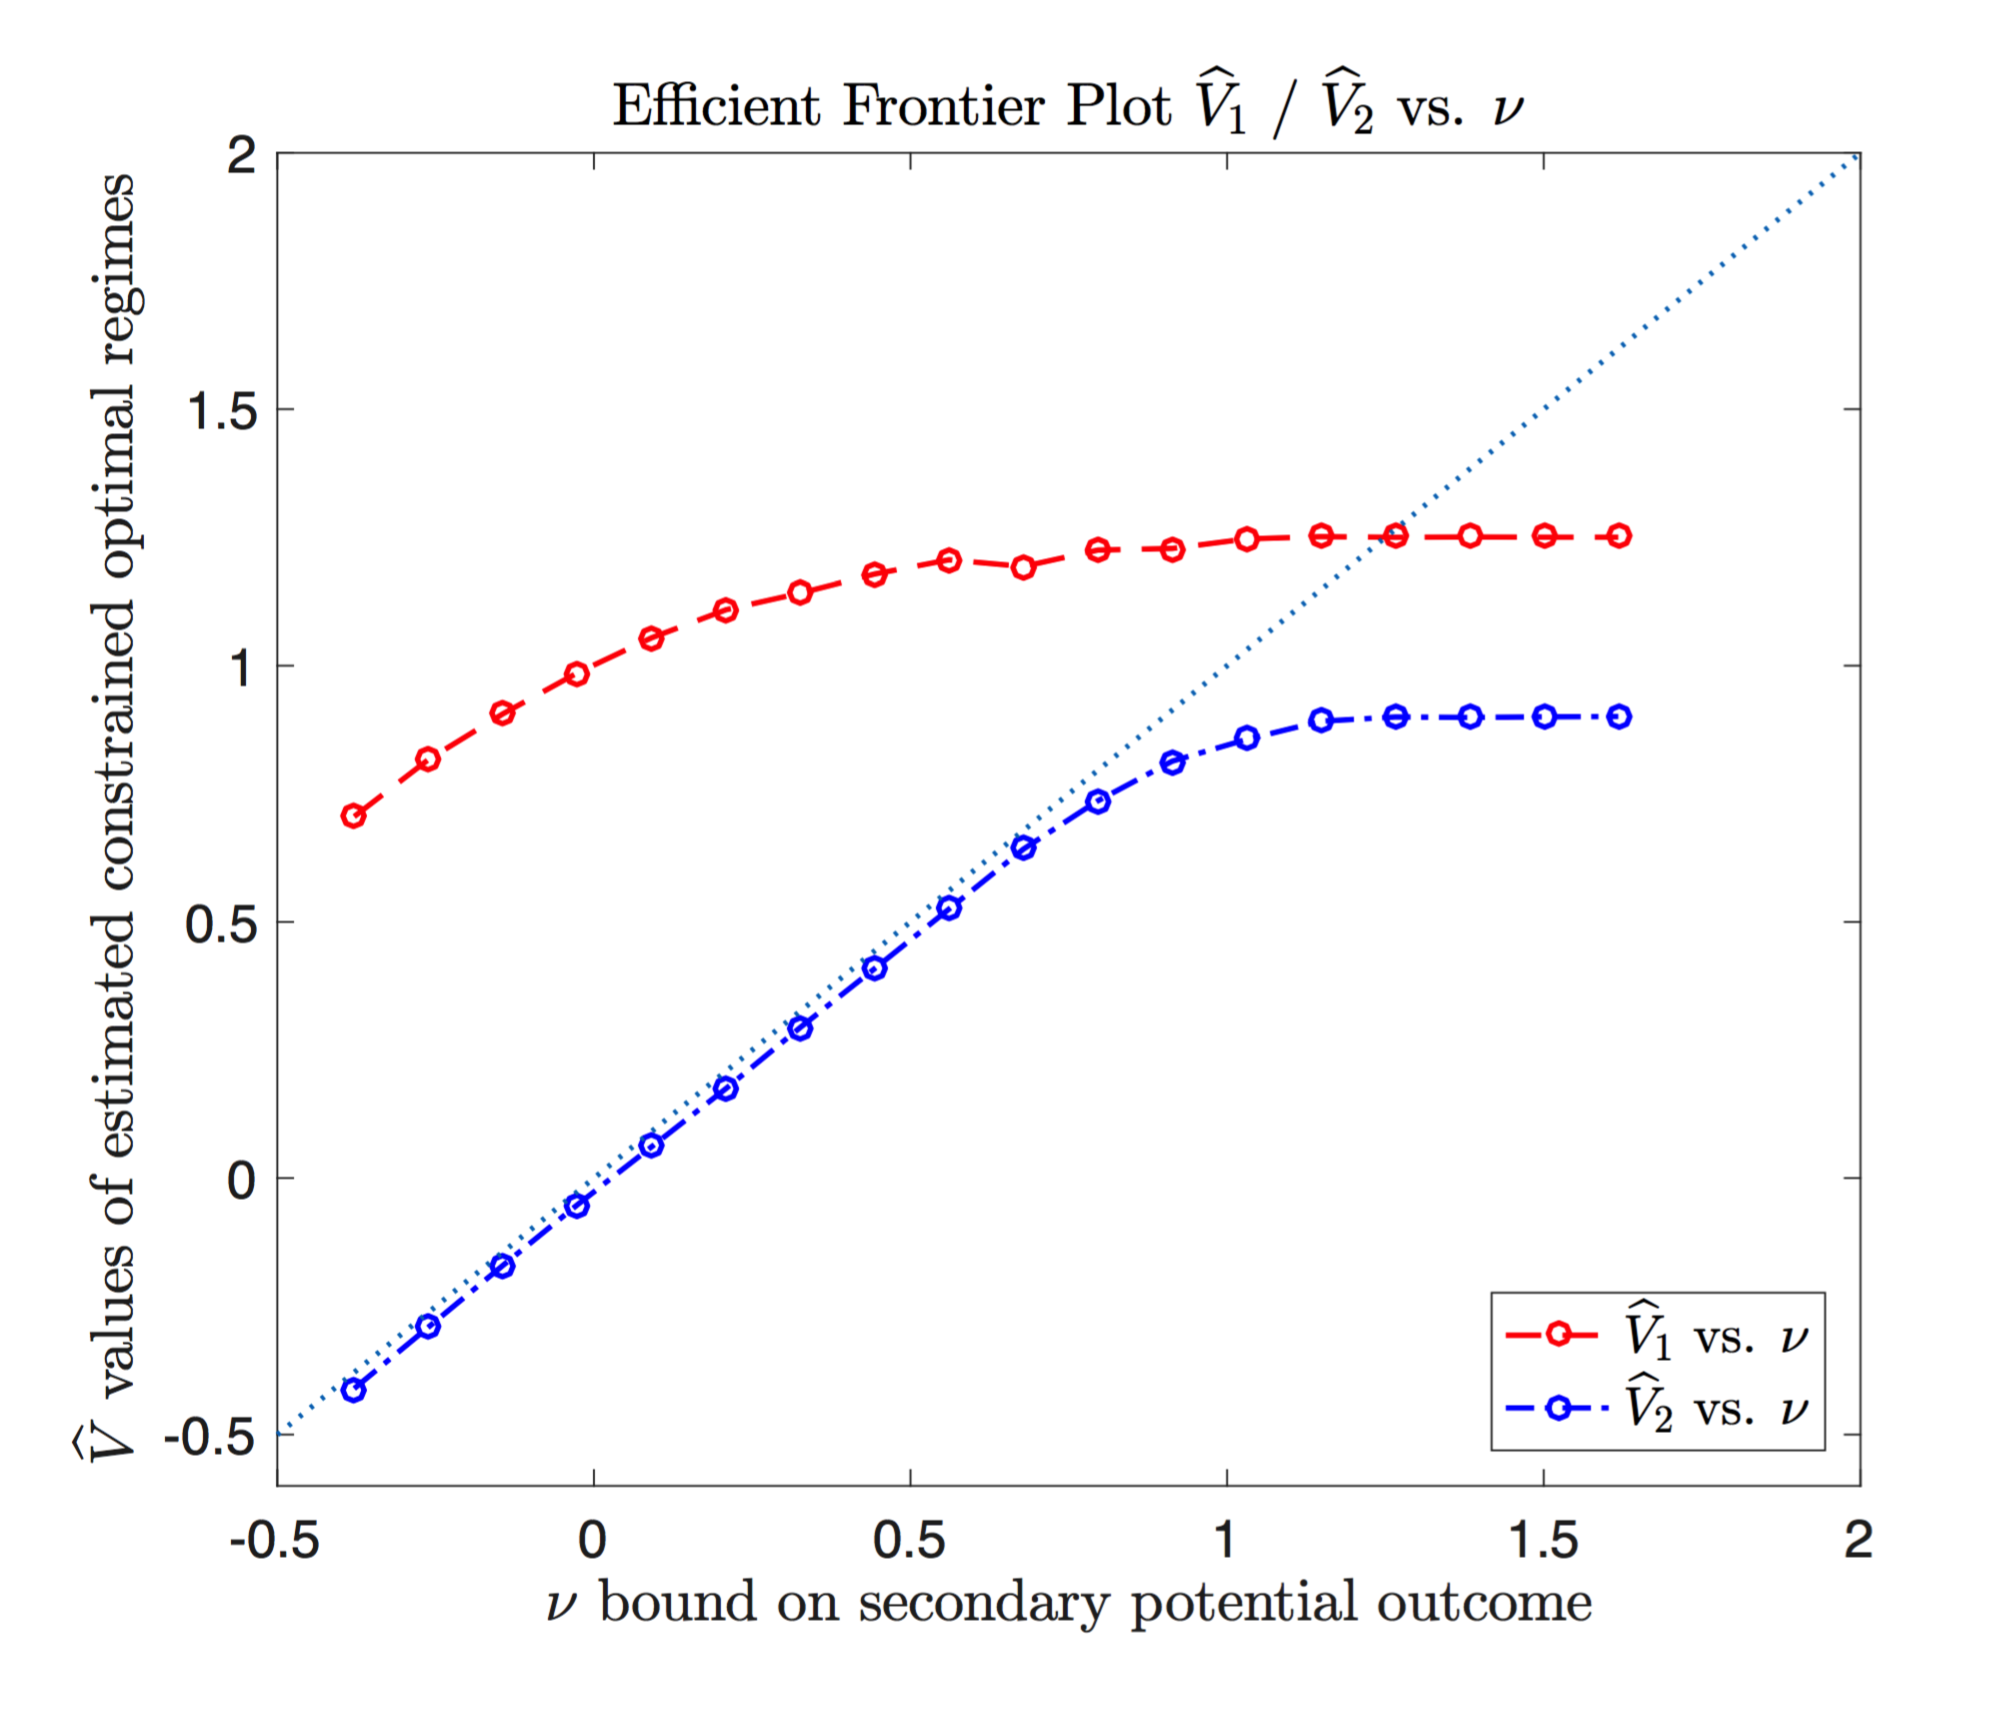
\includegraphics[width=.9\linewidth]{./figs/efficient_plot6.png}
	\caption{Efficient frontier for estimated constrained optimal regimes for Setting 6.}
	\label{fig:6}
	\justify
X-axis is for the values for the constraints $\nu$; Y-axis is for the values of estimated regimes. Red dashed line is for the values in terms of the primary outcome of interest. Blue dashed line is for the values in terms of the secondary outcome of interest.
\end{figure}
\begin{table}[!htbp]
	\caption {Simulation Result for Setting 7}
	\centering
	{\tt
		\begin{tabular}{rrrrrrrrrr}\hline 
setting & $\nu$  & $\wh{V}_1(\wh{\bs{\theta}}_{\nu})$ & $std(\wh{V}_1)$ & $\wh{V}_2(\wh{\bs{\theta}}_{\nu})$ & $std(\wh{V}_2)$ & $\wh{\theta}_{\nu,1}$ & $std(\wh{\theta}_{\nu,1})$ & $\wh{\theta}_{\nu,2}$ & $std(\wh{\theta}_{\nu,2})$ \\ \hline 
7 &    -2.60 &     1.12 &     0.01  &    -3.26 &      0.13 &     -0.69 &      0.11 &      0.71 &      0.10 \\ 
7 &    -2.19 &     1.11 &     0.01  &    -3.26 &      0.15 &     -0.69 &      0.11 &      0.71 &      0.11 \\ 
7 &    -1.77 &     1.11 &     0.01  &    -3.26 &      0.16 &     -0.69 &      0.11 &      0.71 &      0.11 \\ 
7 &    -1.36 &     1.12 &     0.01  &    -3.26 &      0.13 &     -0.69 &      0.11 &      0.70 &      0.11 \\ 
7 &    -0.95 &     1.11 &     0.01  &    -3.25 &      0.16 &     -0.69 &      0.11 &      0.71 &      0.11 \\ 
7 &    -0.54 &     1.11 &     0.01  &    -3.25 &      0.16 &     -0.69 &      0.11 &      0.71 &      0.11 \\ 
7 &    -0.12 &     1.11 &     0.01  &    -3.25 &      0.16 &     -0.69 &      0.11 &      0.71 &      0.11 \\ 
7 &     0.29 &     1.11 &     0.01  &    -3.25 &      0.16 &     -0.69 &      0.11 &      0.71 &      0.11 \\ 
7 &     0.70 &     1.11 &     0.01  &    -3.25 &      0.16 &     -0.69 &      0.12 &      0.71 &      0.11 \\ 
7 &     1.11 &     1.11 &     0.01  &    -3.25 &      0.16 &     -0.68 &      0.11 &      0.71 &      0.11 \\ 
7 &     1.53 &     1.11 &     0.01  &    -3.25 &      0.16 &     -0.69 &      0.11 &      0.71 &      0.11 \\ 
7 &     1.94 &     1.11 &     0.01  &    -3.25 &      0.16 &     -0.69 &      0.11 &      0.71 &      0.11 \\ 
7 &     2.35 &     1.11 &     0.01  &    -3.25 &      0.16 &     -0.69 &      0.11 &      0.71 &      0.11 \\ 
7 &     2.76 &     1.11 &     0.01  &    -3.25 &      0.16 &     -0.69 &      0.11 &      0.71 &      0.11 \\ 
7 &     3.18 &     1.11 &     0.01  &    -3.26 &      0.16 &     -0.69 &      0.11 &      0.71 &      0.11 \\ 
7 &     3.59 &     1.11 &     0.01  &    -3.25 &      0.17 &     -0.68 &      0.11 &      0.71 &      0.11 \\ 
7 &     4.00 &     1.11 &     0.01  &    -3.25 &      0.16 &     -0.69 &      0.11 &      0.71 &      0.11 \\ 
7 &     4.41 &     1.11 &     0.09  &    -3.21 &      0.56 &     -0.68 &      0.15 &      0.70 &      0.14 \\ \hline 
\end{tabular}

	}
	\justify
	Here, $\nu$ denotes the values of the constraint; $\wh{V}_1(\wh{\bs{\theta}}_{\nu})$ denotes the values of estimated regimes in terms of primary outcome of interest; $std(\wh{V}_1)$ denotes the standard deviation of the estimated regime values in terms of primary outcome of interest; $\wh{V}_2(\wh{\bs{\theta}}_{\nu})$ denotes the values of estimated regimes in terms of secondary outcome of interest; $std(\wh{V}_2)$ denotes the standard deviation of the estimated regime values in terms of secondary outcome of interest; $\wh{\theta}_{\nu,1}$ and $\wh{\theta}_{\nu,2}$ denote the estimated index parameters of the regimes; $std(\wh{\theta}_{\nu,1})$ and $std(\wh{\theta}_{\nu,2})$ denote the standard deviations of those estimated index parameters.	
\end{table} 
\begin{figure}[!htb]
	\centering
	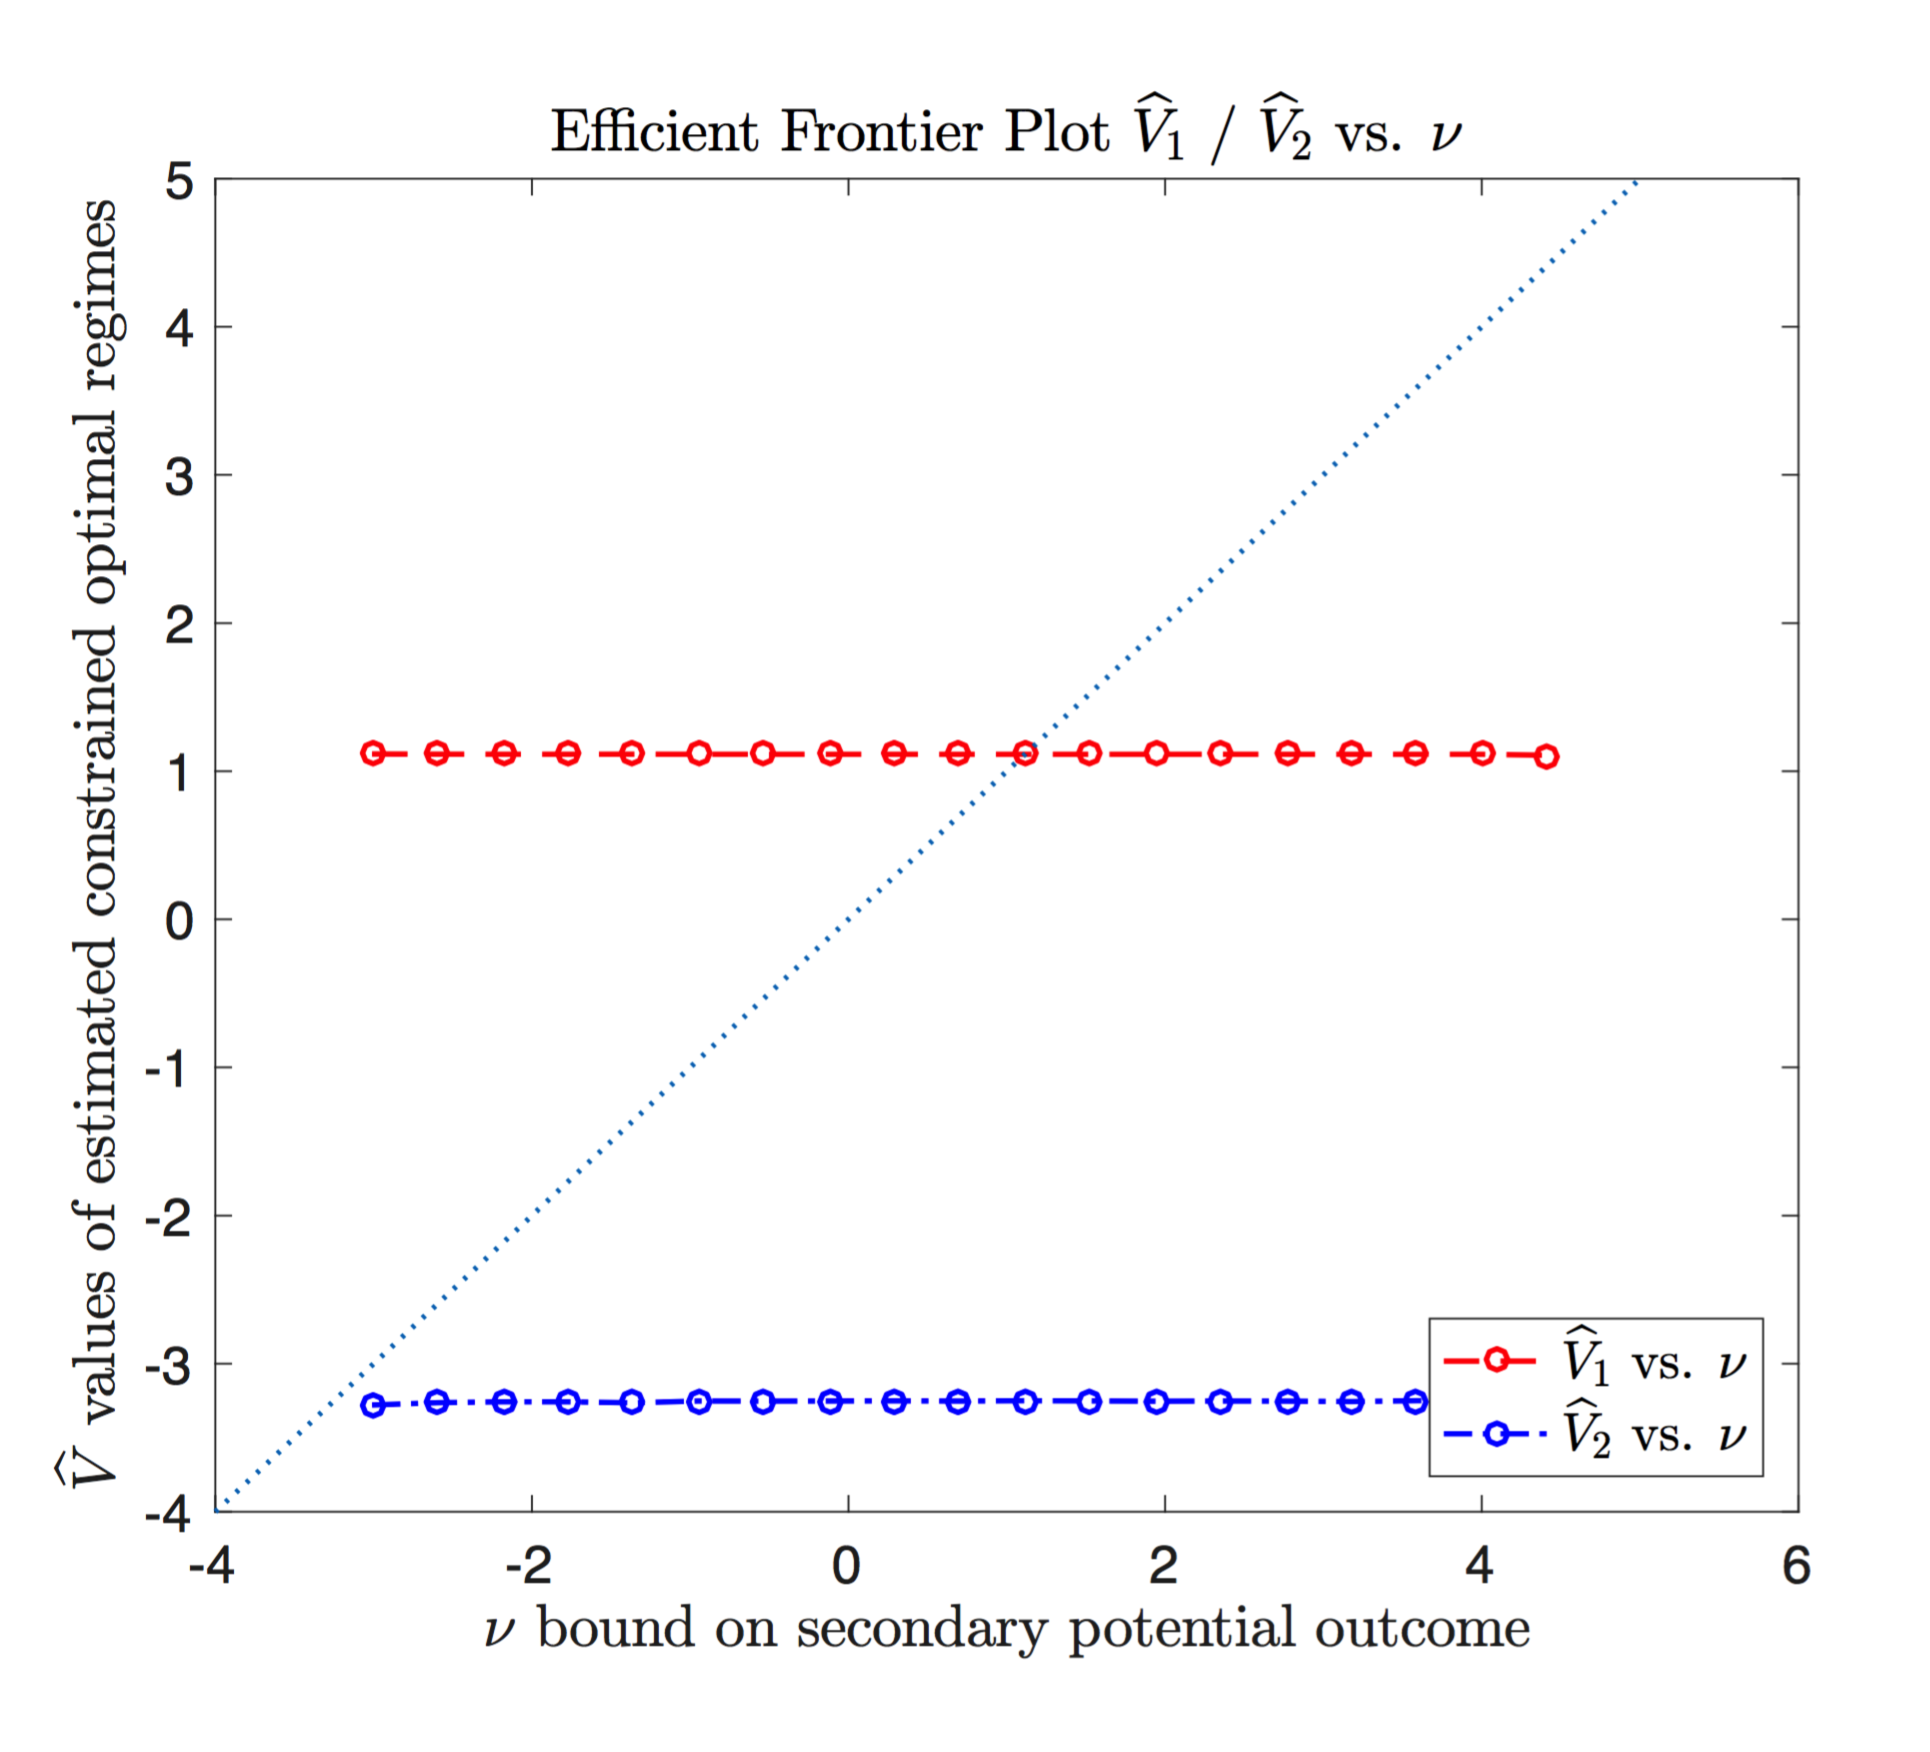
\includegraphics[width=.9\linewidth]{./figs/efficient_plot7.png}
	\caption{Efficient frontier for estimated constrained optimal regimes for Setting 7.}
	\label{fig:7}
	\justify
X-axis is for the values for the constraints $\nu$; Y-axis is for the values of estimated regimes. Red dashed line is for the values in terms of the primary outcome of interest. Blue dashed line is for the values in terms of the secondary outcome of interest.
\end{figure}
\begin{table}[!htbp]
	\caption {Simulation Result for Setting 8}
	\centering
	{\tt
		\begin{tabular}{rrrrrrrrrr}\hline 
$\nu$  & $\wh{V}_1(\wh{\bs{\theta}}_{\nu})$ & $std(\wh{V}_1)$ & $\wh{V}_2(\wh{\bs{\theta}}_{\nu})$ & $std(\wh{V}_2)$ & $\wh{\theta}_{\nu,1}$ & $std(\wh{\theta}_{\nu,1})$ & $\wh{\theta}_{\nu,2}$ & $std(\wh{\theta}_{\nu,2})$ \\ \hline 
%8 &      NaN &      NaN &      NaN  &      NaN &       NaN &       NaN &       NaN &       NaN &       NaN \\ 
%8 &      NaN &      NaN &      NaN  &      NaN &       NaN &       NaN &       NaN &       NaN &       NaN \\ 
%8 &    -3.19 &      NaN &      NaN  &      NaN &       NaN &       NaN &       NaN &       NaN &       NaN \\ 
-2.80 &    -0.36 &     0.33  &    -2.85 &      0.12 &      0.78 &      0.05 &     -0.63 &      0.06 \\ 
-2.41 &     0.54 &     0.26  &    -2.44 &      0.14 &      0.64 &      0.04 &     -0.77 &      0.04 \\ 
-2.02 &     1.24 &     0.22  &    -2.05 &      0.14 &      0.51 &      0.05 &     -0.86 &      0.03 \\ 
-1.64 &     1.82 &     0.21  &    -1.66 &      0.15 &      0.39 &      0.04 &     -0.92 &      0.02 \\ 
-1.25 &     2.35 &     0.19  &    -1.24 &      0.16 &      0.27 &      0.04 &     -0.96 &      0.01 \\ 
-0.86 &     2.82 &     0.17  &    -0.84 &      0.16 &      0.15 &      0.04 &     -0.99 &      0.01 \\ 
-0.47 &     3.18 &     0.50  &    -0.44 &      0.15 &      0.05 &      0.05 &     -0.99 &      0.13 \\ 
-0.08 &     3.51 &     0.51  &    -0.08 &      0.15 &     -0.06 &      0.05 &     -0.99 &      0.13 \\ 
 0.31 &     3.75 &     0.86  &     0.30 &      0.17 &     -0.16 &      0.07 &     -0.96 &      0.24 \\ 
 0.70 &     3.92 &     1.21  &     0.71 &      0.16 &     -0.26 &      0.09 &     -0.90 &      0.33 \\ 
 1.09 &     4.16 &     1.19  &     1.10 &      0.16 &     -0.36 &      0.08 &     -0.87 &      0.33 \\ 
 1.47 &     4.30 &     1.32  &     1.51 &      0.16 &     -0.45 &      0.09 &     -0.81 &      0.37 \\ 
 1.86 &     4.22 &     1.74  &     1.88 &      0.15 &     -0.53 &      0.12 &     -0.69 &      0.48 \\ 
 2.25 &     3.73 &     2.35  &     2.26 &      0.15 &     -0.59 &      0.15 &     -0.45 &      0.65 \\ 
 2.64 &     4.44 &     1.50  &     2.65 &      0.11 &     -0.71 &      0.09 &     -0.56 &      0.42 \\ 
 3.03 &     4.79 &     0.64  &     2.74 &      0.06 &     -0.75 &      0.04 &     -0.63 &      0.19 \\ 
 3.42 &     4.67 &     0.92  &     2.76 &      0.15 &     -0.75 &      0.03 &     -0.59 &      0.30 \\ 
 3.81 &     4.81 &     0.44  &     2.75 &      0.14 &     -0.75 &      0.01 &     -0.64 &      0.16 \\ 
 4.20 &     4.85 &     0.15  &     2.74 &      0.12 &     -0.75 &      0.02 &     -0.65 &      0.07 \\ \hline 
\end{tabular}

	}
	\justify
	Here, $\nu$ denotes the values of the constraint; $\wh{V}_1(\wh{\bs{\theta}}_{\nu})$ denotes the values of estimated regimes in terms of primary outcome of interest; $std(\wh{V}_1)$ denotes the standard deviation of the estimated regime values in terms of primary outcome of interest; $\wh{V}_2(\wh{\bs{\theta}}_{\nu})$ denotes the values of estimated regimes in terms of secondary outcome of interest; $std(\wh{V}_2)$ denotes the standard deviation of the estimated regime values in terms of secondary outcome of interest; $\wh{\theta}_{\nu,1}$ and $\wh{\theta}_{\nu,2}$ denote the estimated index parameters of the regimes; $std(\wh{\theta}_{\nu,1})$ and $std(\wh{\theta}_{\nu,2})$ denote the standard deviations of those estimated index parameters.	
\end{table} 
\begin{figure}[!htb]
	\centering
	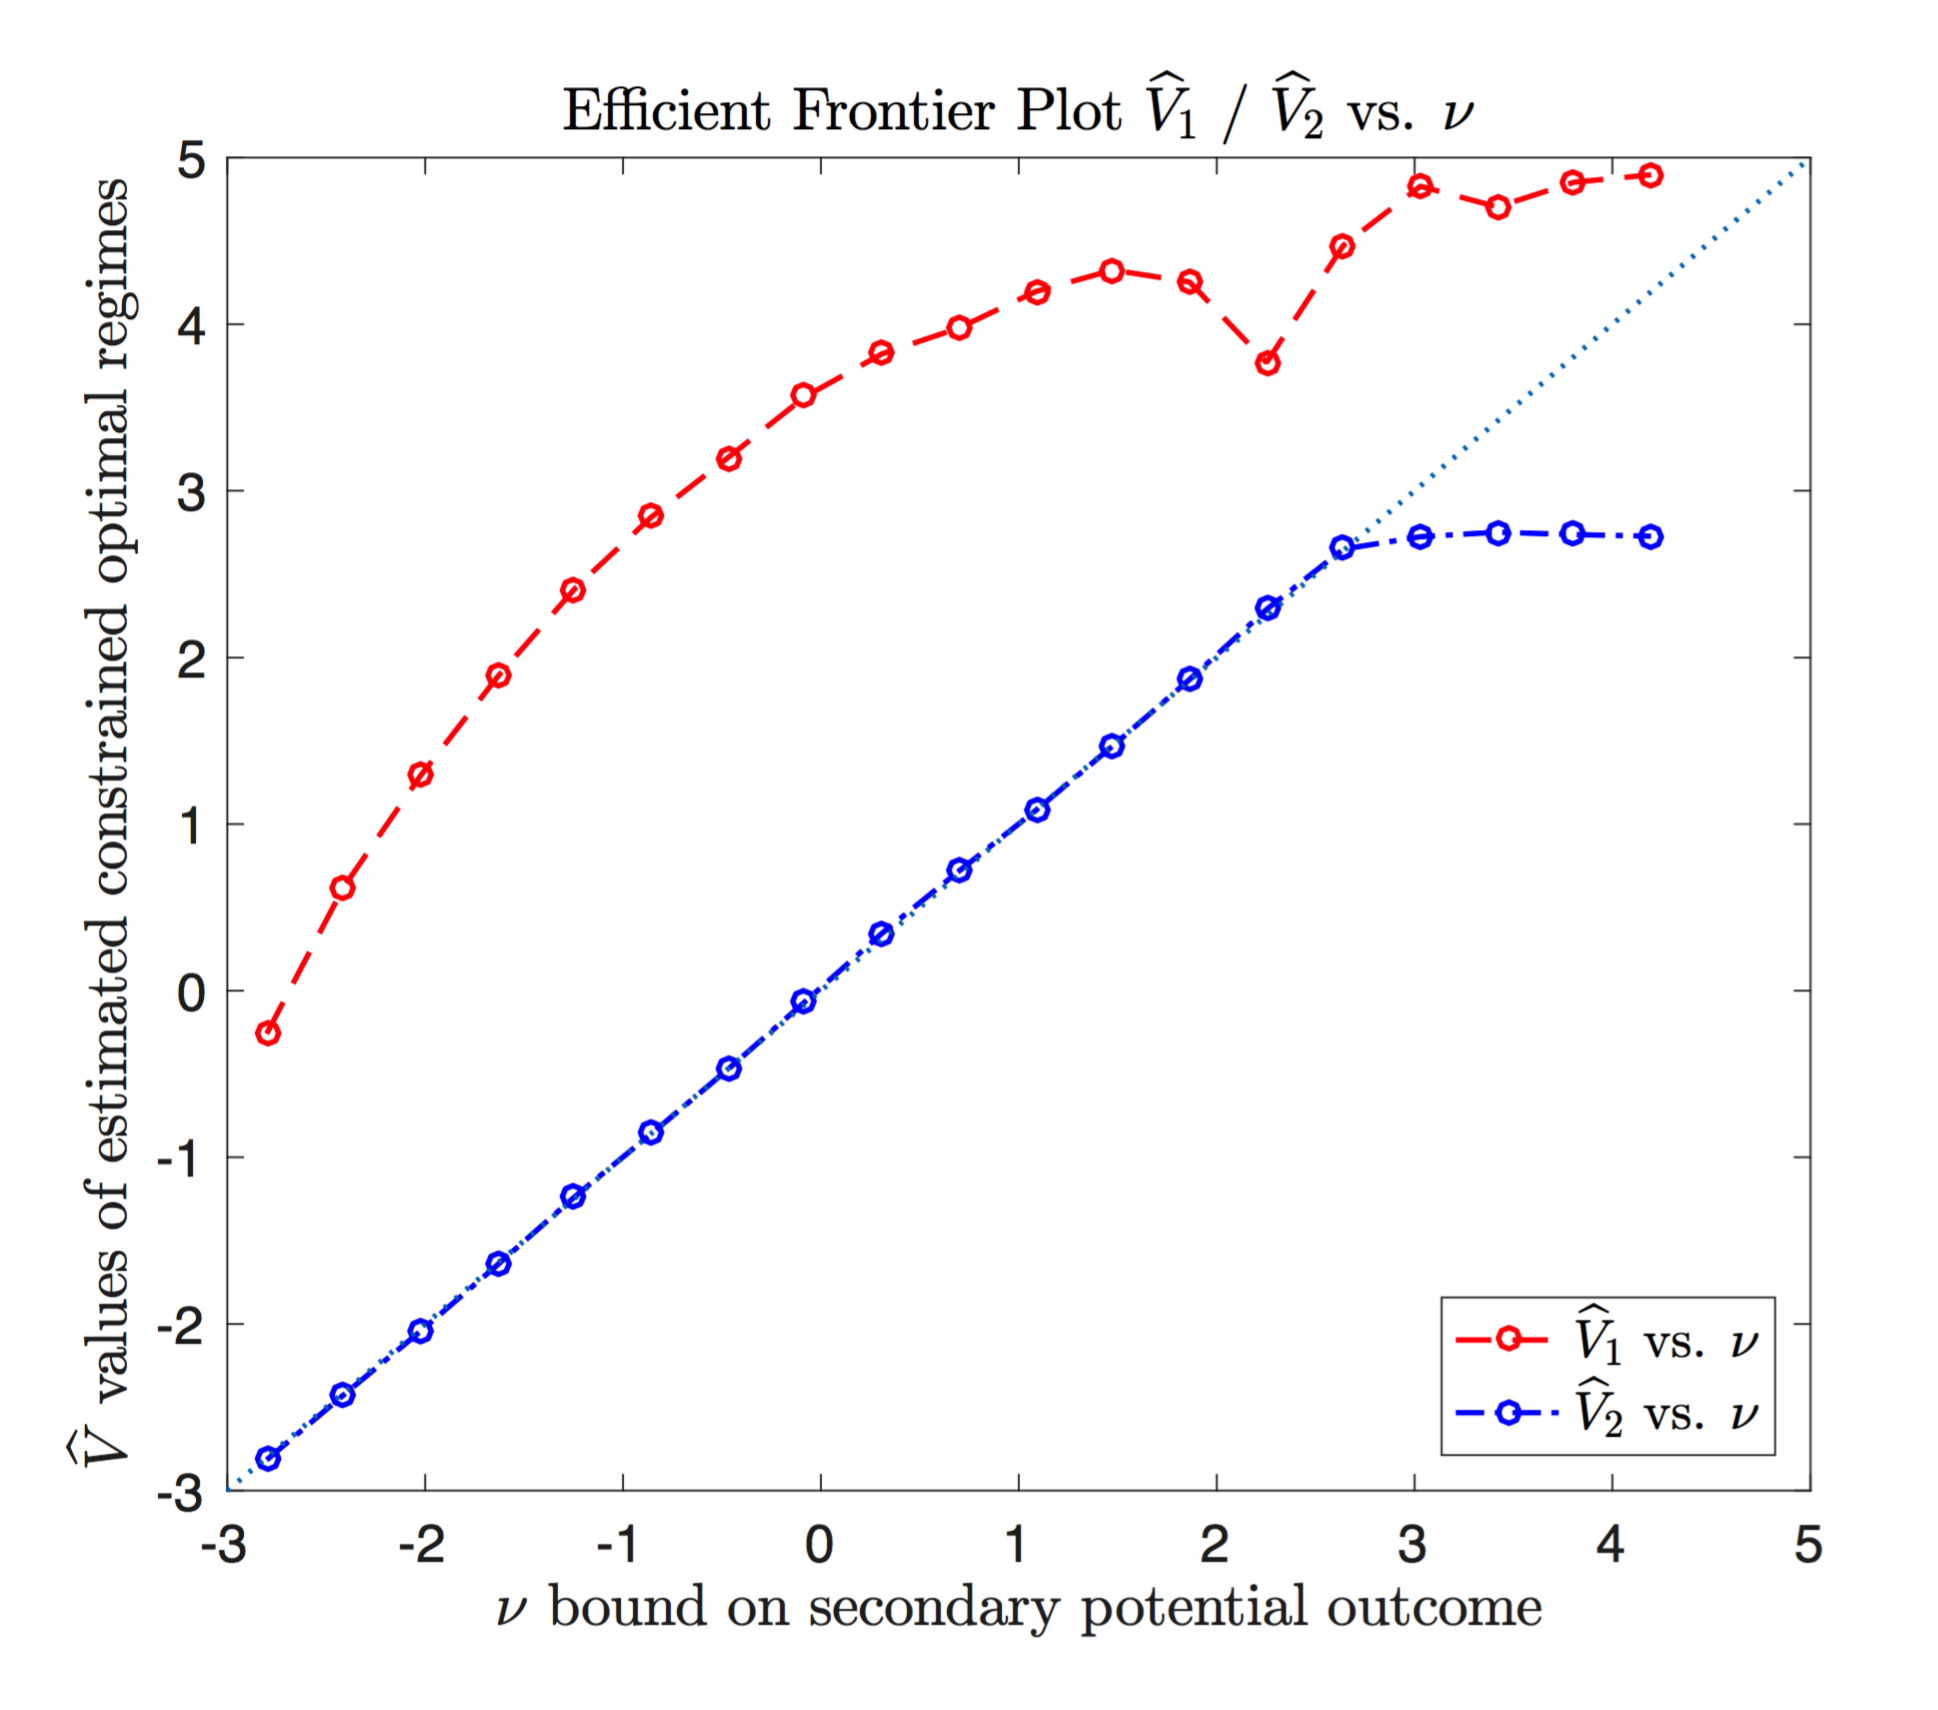
\includegraphics[width=.9\linewidth]{./figs/efficient_plot8.png}
	\caption{Efficient frontier for estimated constrained optimal regimes for Setting 8.}
	\label{fig:8}
	\justify
X-axis is for the values for the constraints $\nu$; Y-axis is for the values of estimated regimes. Red dashed line is for the values in terms of the primary outcome of interest. Blue dashed line is for the values in terms of the secondary outcome of interest.
\end{figure}
\begin{table}[!htbp]
	\caption {Simulation Result for Setting 9}
	\centering
	{\tt
		\begin{tabular}{rrrrrrrrrr}\hline 
 $\nu$  & $\wh{V}_1(\wh{\bs{\theta}}_{\nu})$ & $std(\wh{V}_1)$ & $\wh{V}_2(\wh{\bs{\theta}}_{\nu})$ & $std(\wh{V}_2)$ & $\wh{\theta}_{\nu,1}$ & $std(\wh{\theta}_{\nu,1})$ & $\wh{\theta}_{\nu,2}$ & $std(\wh{\theta}_{\nu,2})$ \\ \hline 
-0.70 &     3.32 &     1.24  &    -0.97 &      0.63 &      0.75 &      0.04 &     -0.66 &      0.05 \\ 
-0.56 &     3.72 &     0.01  &    -0.77 &      0.02 &      0.73 &      0.04 &     -0.68 &      0.04 \\ 
-0.41 &     3.72 &     0.01  &    -0.77 &      0.02 &      0.73 &      0.04 &     -0.68 &      0.04 \\ 
-0.27 &     3.72 &     0.01  &    -0.77 &      0.02 &      0.73 &      0.04 &     -0.68 &      0.04 \\ 
-0.13 &     3.72 &     0.01  &    -0.77 &      0.02 &      0.73 &      0.04 &     -0.68 &      0.04 \\ 
 0.01 &     3.72 &     0.01  &    -0.77 &      0.02 &      0.73 &      0.04 &     -0.68 &      0.04 \\ 
 0.15 &     3.72 &     0.01  &    -0.77 &      0.02 &      0.73 &      0.04 &     -0.68 &      0.04 \\ 
 0.29 &     3.72 &     0.01  &    -0.77 &      0.02 &      0.73 &      0.04 &     -0.68 &      0.04 \\ 
 0.43 &     3.72 &     0.01  &    -0.77 &      0.02 &      0.73 &      0.04 &     -0.68 &      0.04 \\ 
 0.58 &     3.72 &     0.01  &    -0.77 &      0.02 &      0.73 &      0.04 &     -0.68 &      0.04 \\ 
 0.72 &     3.72 &     0.01  &    -0.77 &      0.02 &      0.73 &      0.04 &     -0.68 &      0.04 \\ 
 0.86 &     3.72 &     0.01  &    -0.77 &      0.02 &      0.73 &      0.04 &     -0.68 &      0.04 \\ 
 1.00 &     3.72 &     0.01  &    -0.77 &      0.02 &      0.73 &      0.04 &     -0.68 &      0.04 \\ 
 1.14 &     3.72 &     0.01  &    -0.77 &      0.02 &      0.73 &      0.04 &     -0.68 &      0.04 \\ 
 1.28 &     3.72 &     0.01  &    -0.77 &      0.02 &      0.73 &      0.04 &     -0.68 &      0.04 \\ 
 1.43 &     3.72 &     0.01  &    -0.77 &      0.02 &      0.73 &      0.04 &     -0.68 &      0.04 \\ 
 1.57 &     3.72 &     0.01  &    -0.77 &      0.02 &      0.73 &      0.04 &     -0.68 &      0.04 \\ 
 1.71 &     3.72 &     0.01  &    -0.77 &      0.02 &      0.73 &      0.04 &     -0.68 &      0.04 \\ 
 1.85 &     3.72 &     0.01  &    -0.77 &      0.02 &      0.73 &      0.04 &     -0.68 &      0.04 \\ \hline 
\end{tabular}

	}
	\justify
	Here, $\nu$ denotes the values of the constraint; $\wh{V}_1(\wh{\bs{\theta}}_{\nu})$ denotes the values of estimated regimes in terms of primary outcome of interest; $std(\wh{V}_1)$ denotes the standard deviation of the estimated regime values in terms of primary outcome of interest; $\wh{V}_2(\wh{\bs{\theta}}_{\nu})$ denotes the values of estimated regimes in terms of secondary outcome of interest; $std(\wh{V}_2)$ denotes the standard deviation of the estimated regime values in terms of secondary outcome of interest; $\wh{\theta}_{\nu,1}$ and $\wh{\theta}_{\nu,2}$ denote the estimated index parameters of the regimes; $std(\wh{\theta}_{\nu,1})$ and $std(\wh{\theta}_{\nu,2})$ denote the standard deviations of those estimated index parameters.	
\end{table} 
\begin{figure}[!htb]
	\centering
	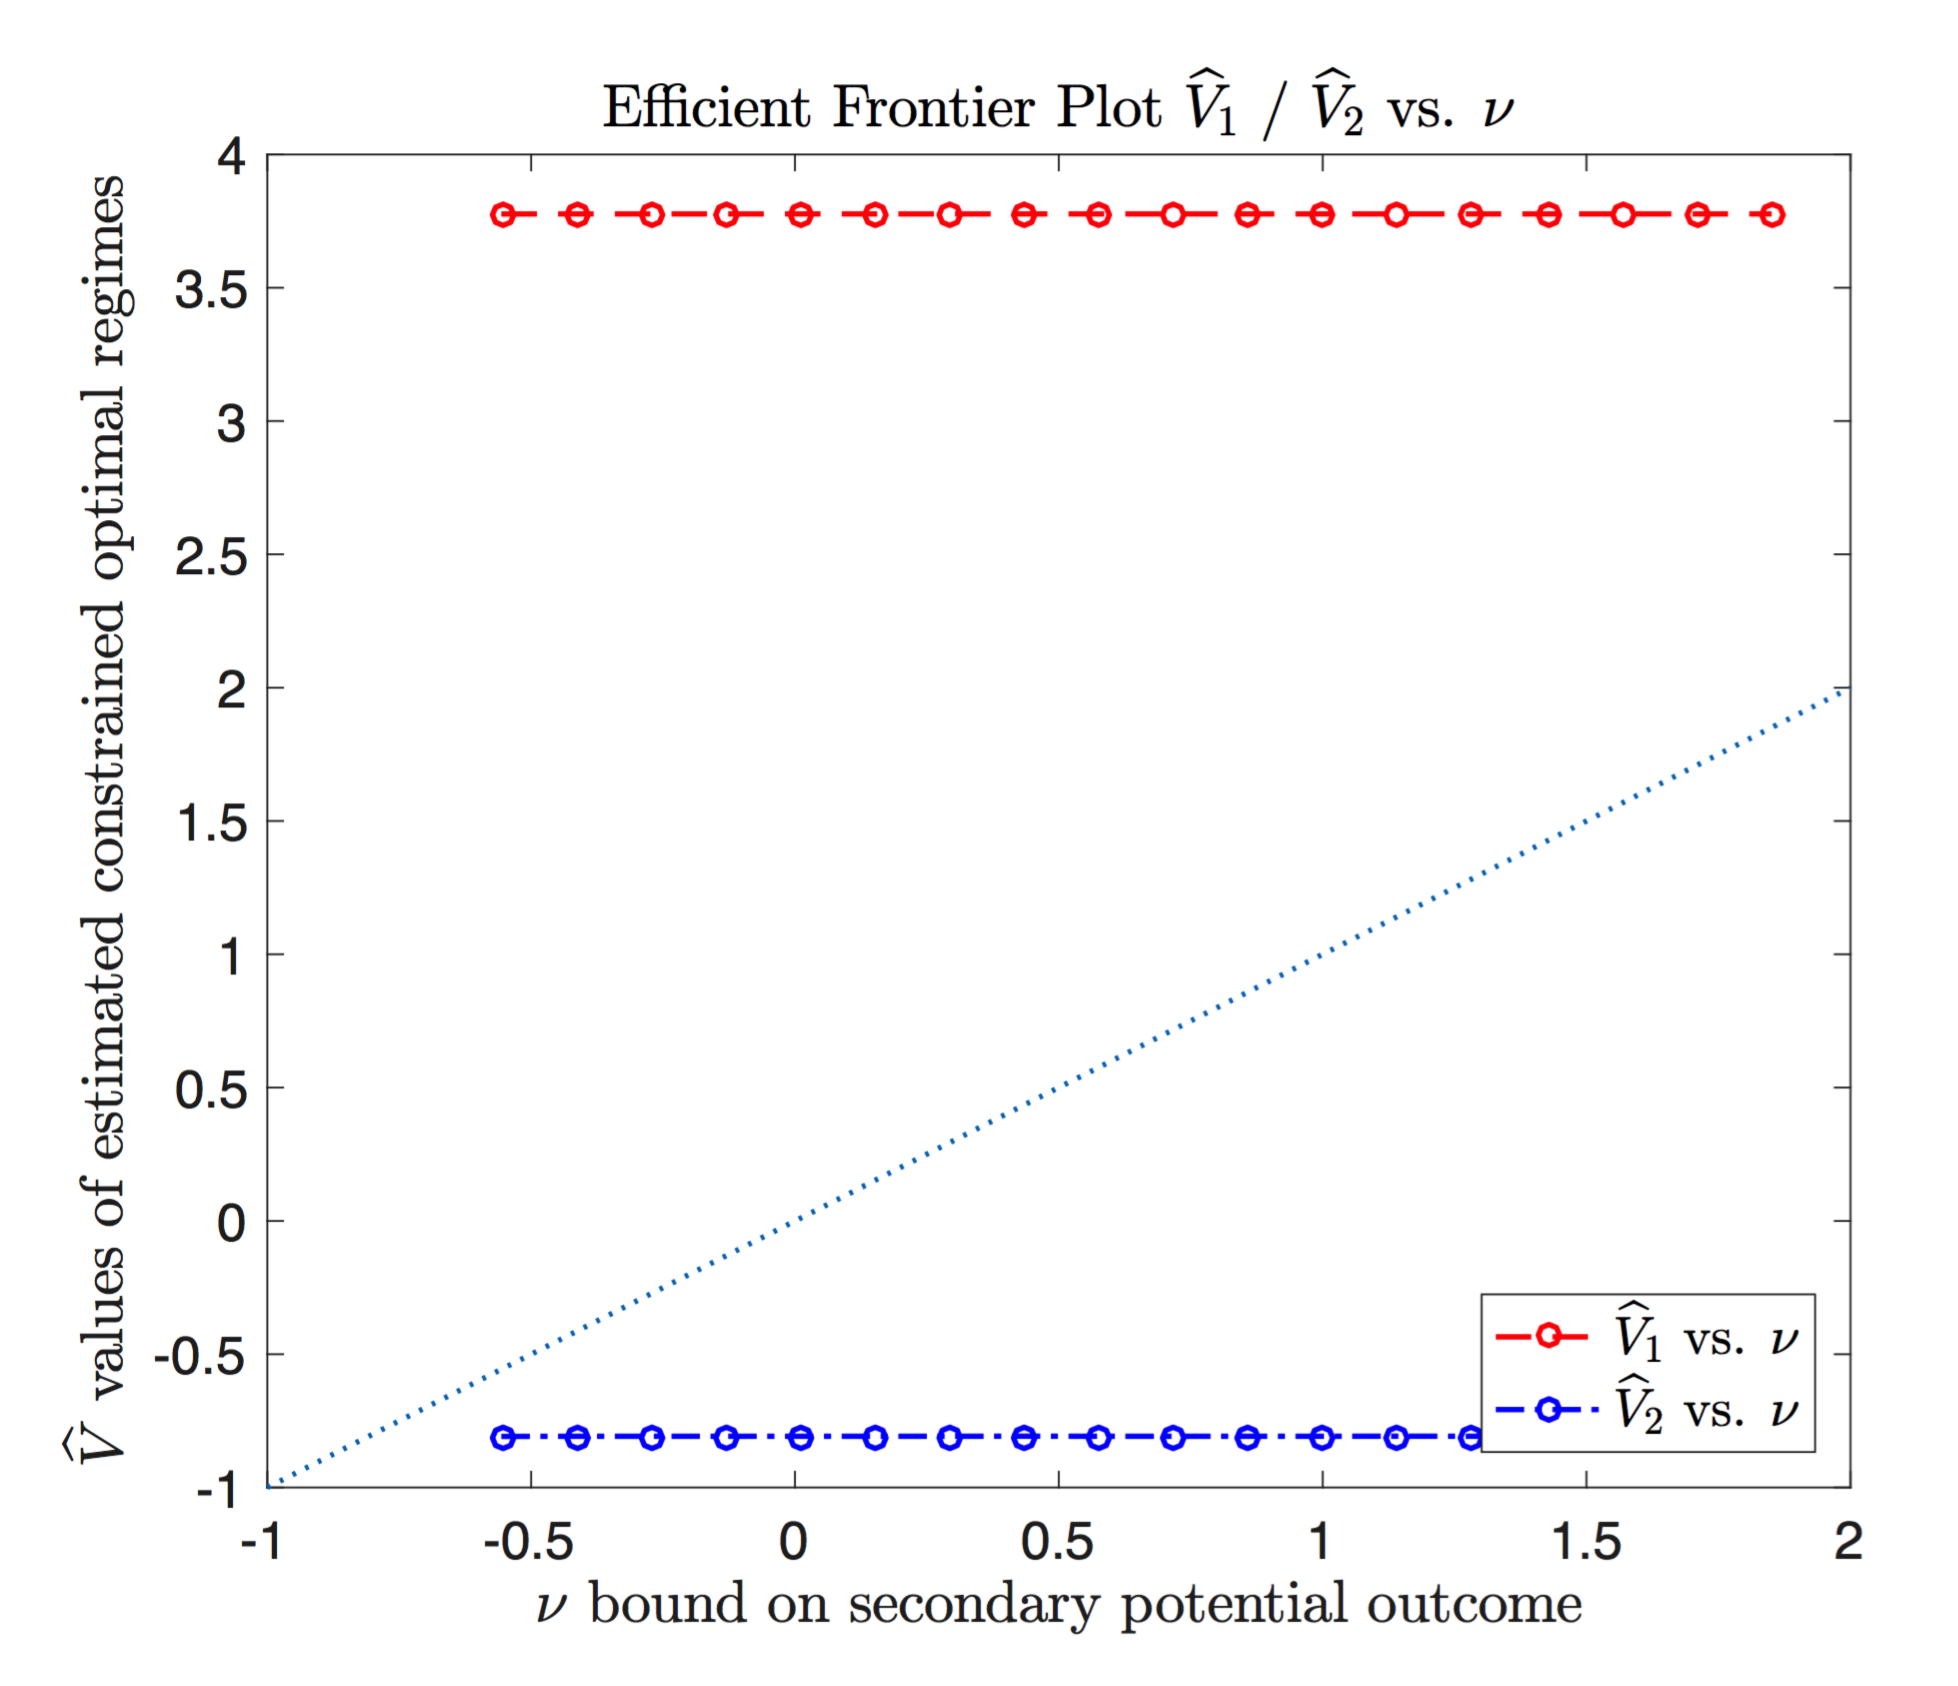
\includegraphics[width=.9\linewidth]{./figs/efficient_plot9.png}
	\caption{Efficient frontier for estimated constrained optimal regimes for Setting 9.}
	\label{fig:9}
	\justify
X-axis is for the values for the constraints $\nu$; Y-axis is for the values of estimated regimes. Red dashed line is for the values in terms of the primary outcome of interest. Blue dashed line is for the values in terms of the secondary outcome of interest.
\end{figure}
%	{\centering
%		\begin{minipage}{0.45\textwidth}
%			\centering
%			%%%\includegraphics[width=.9\linewidth]{lb9.pdf}
%			\captionof{figure}{Setting 9 by log barrier method}
%		\end{minipage}
%		\begin{minipage}{0.45\textwidth}
%			\centering
%			%%%\includegraphics[width=.9\linewidth]{ex9.pdf}
%			\captionof{figure}{Setting 9 by exact penalty method}
%		\end{minipage}
%	}\\
\end{appendices}
\end{document}